% Achard, Gajdos Preuss & Servant -- working copy, converted from the Word revision.
%
% CHANGE MARKING. The Word copy this is converted from is colour-coded against
% "Achard et al R1_v3.docx": text already in that version keeps its own colour, text added
% since is blue, and struck runs are proposed deletions. The three macros below carry that
% marking. For a clean copy, redefine them:
%     \renewcommand{\new}[1]{#1}\renewcommand{\old}[1]{#1}\renewcommand{\del}[1]{}
\documentclass[a4paper,11pt]{article}
\usepackage[T1]{fontenc}
% Latin Modern rather than the T1 Computer Modern bitmaps: microtype's font expansion
% needs a scalable font, and a TeX Live without cm-super installed fails outright on it.
\usepackage{lmodern}
\usepackage[utf8]{inputenc}
\usepackage[english]{babel}
\usepackage[top=2cm,bottom=2.2cm,left=3cm,right=3cm]{geometry}
\usepackage[onehalfspacing]{setspace}
\usepackage{amsmath,amssymb,amsfonts,amsthm}
\usepackage{mathtools}
\usepackage{bbm}
\usepackage{graphicx}
\graphicspath{{figures/}}
\usepackage{array}          % >{...} column prefixes, used by the wide tables
\usepackage{booktabs}
\usepackage{caption}
% Figures and tables are not floats here -- the journal layout collects them in their own
% sections -- so \captionof carries the numbering, and every one of them has a \label.
% The Supplemental Material section restarts both counters with an S prefix.
\captionsetup{labelfont=bf,labelsep=period,singlelinecheck=false,justification=raggedright}
\captionsetup[figure]{name=Fig}
\captionsetup[table]{name=Table}
% Appendix statements: one shared counter, so they read A.1, A.2, ... in order.
\theoremstyle{definition}
\newtheorem{proposition}{Proposition}
\renewcommand{\theproposition}{A.\arabic{proposition}}
\newtheorem{corollary}[proposition]{Corollary}
\newtheorem{remark}[proposition]{Remark}
\usepackage{xcolor}
\usepackage[normalem]{ulem}
\usepackage{microtype}
\usepackage{lineno}
\allowdisplaybreaks
% NOT \mathtoolsset{showonlyrefs}, which note4.tex uses: it prints a number only on an
% equation some \eqref points at. Every displayed equation here is either referenced by
% \eqref or deliberately unnumbered (equation*), and the Appendix reprints three of the
% Results equations under their original numbers via a tag pointing at the original label
% would break.
\usepackage{hyperref}
% hidelinks, not coloured links: this copy uses colour to mark revisions, and a
% blue \cite in the middle of a red sentence reads as new material rather than as a
% link. Links stay live, they just take the colour of the text around them.
\hypersetup{hidelinks}
% The OSF link is one unbreakable token, and the A4 measure is narrower than the letter
% one was, so it now runs into the margin; xurl lets a URL break anywhere.
\usepackage{xurl}

% Bibliography: biblatex + biber with the APA style, the same setup note4.tex uses, so
% both documents cite the same Zotero library the same way. This needs biber, not bibtex
% -- see README for the build order.
\usepackage[style=apa]{biblatex}
\DeclareLanguageMapping{english}{english-apa}
\addbibresource{bib.bib}

% The macros note4.tex defines, so the two documents read alike and an equation edited
% by hand here can be written the same way. omml2tex emits \Var, \Cov and \dd for the
% operators Word stores as upright runs.
\newcommand{\R}{\mathbb R}
\newcommand{\E}{\mathbb E}
\renewcommand{\P}{\mathbb P}
\newcommand{\Var}{\operatorname{Var}}
\newcommand{\Cov}{\operatorname{Cov}}
\newcommand{\dd}{\mathrm d}
\newcommand{\RT}{\mathrm{RT}}
\newcommand{\nustat}{{\nu }_{\mathrm{stat}}}
\newcommand{\bigO}{\mathcal{O}}
\newcommand{\1}{\mathbbm{1}}
\newcommand{\indep}{\perp\!\!\!\perp}
\DeclareMathOperator{\sgn}{sgn}
\newcommand\poscite[1]{\citeauthor{#1}'s (\citeyear{#1})}

% Robust, because these appear inside \section arguments: 38 of the 58 headings carry
% revision colour in the docx, and stripping it there -- which an earlier version of the
% converter did -- silently lost the marking on more than half the headings.
% ... and colour means nothing in a PDF bookmark, so the macros flatten there.

% The printed reference list now comes from biblatex, so body.tex no longer uses this
% environment. It is kept because references_verbatim.tex -- the APA text exactly as Word
% carried it, which checkbib.py reads -- can be \input to set the two lists side by side.
% \everypar rather than a negative \parindent, which \parskip and the surrounding
% zero-indent setting between them cancel out.
\newenvironment{references}
  % \sloppy is load-bearing here. A DOI is one unbreakable word, so a reference ending
  % in a long one has nowhere to break: without \sloppy, eleven of them overrun the
  % margin, one by 136pt. With it, TeX stretches the spaces instead -- five lines come
  % out loose, the worst being Rogge et al. Loose beats off the page. (xurl is loaded
  % for the OSF link, but it makes no difference here -- \sloppy already absorbs these.)
  {\par\sloppy\setlength{\parindent}{0pt}\everypar{\hangindent=0.4in\hangafter=1}}
  {\par}

% The appendix statements carry their own counter (A.1, A.2, ...), so LaTeX's section
% numbers would give the same material two competing numberings. The Word original has
% no section numbers either.
\setcounter{secnumdepth}{0}

% A last-resort stretch, rather than letting a paragraph overrun. It is needed because
% a word that already contains a hyphen -- "evidence-accumulation" -- can only break
% at that hyphen, and on the narrower A4 measure that break point is sometimes past
% the margin. TeX uses this only on lines it cannot set otherwise.
\setlength{\emergencystretch}{1em}

\setlength{\parskip}{0.5\baselineskip}
\setlength{\parindent}{0pt}
\renewcommand{\thesection}{\arabic{section}}

\title{Graded Motor-Preparatory Dynamics Preserve Perceptual Decisions over Short Delays}
\date{}

\begin{document}
\linenumbers
\textbf{Graded Motor-Preparatory Dynamics Preserve Perceptual Decisions over Short Delays}

Johan A. Achard\textsuperscript{1}, Thibault Gajdos Preuss\textsuperscript{2}, Mathieu Servant\textsuperscript{1}

\textsuperscript{1} Laboratoire de Recherches Int\'egratives en Neurosciences et Psychologie Cognitive, Institut National de la Sant\'e et de la Recherche M\'edicale, Universit\'e Marie et Louis Pasteur

\textsuperscript{2}  Centre de Recherche en Psychologie et Neuroscience, Centre National de la Recherche Scientifique, Aix-Marseille Universit\'e

Abbreviated title:

Perceptual Decisions over Short Delays

Corresponding Author: \url{mathieu.servant@umlp.fr}

Number of pages: 43

Number of figures: 4 (plus 3 supplementary)

Number of tables: 2 (plus 1 appendix table and 6 supplementary)

Number of multimedia and 3D models: 0

Number of words for abstract: 248

Number of words for introduction: 614

Number of words for discussion: 1345

Conflict of interest statement: The authors have no conflicts of interest to  declare.

Acknowledgments:  This work was funded by the European Union (ERC Starting Grant ITDA n$^{\circ}$101039226 allocated to MS). Views and opinions expressed are however those of the author(s) only and do not necessarily reflect those of the European Union or the European Research Council. Neither the European Union nor the granting authority can be held responsible for them.

Data availability: Empirical data and analysis code are freely available on the Open Science Framework  (\url{https://osf.io/86cbw/overview?view\_only=1f47b76612334dc082318a501fda5a4c}).


\textbf{Abstract}

In delayed perceptual reports, the decision is formed before action is permitted, yet response time from the response signal still depends on sensory evidence. This paradox raises the possibility that evidence accumulation leaves a graded trace in motor preparatory circuits rather than ending in a discrete stored choice. We tested this hypothesis in 22 adults of both sexes (17 women) performing a response-signal random-dot motion task with electroencephalography and electromyography. Participants judged motion direction, withheld the selected response for 3 s, and executed it when the response signal was presented; motion coherence and duration were manipulated. Response time increased when coherence or duration decreased.  Fractionating response time at muscle-activation onset showed that these effects were confined to the premotor period. Muscle activations that did not produce overt responses provided a peripheral readout of motor preparation: they were effector-selective, built up during stimulus presentation at a coherence-dependent rate, and continued to ramp during the stimulus-free delay, but no longer at a coherence-dependent build-up rate. These results support an account in which accumulated motion evidence is transmitted to motor preparatory circuits, transformed into a sustained state maintaining the selected response, and shaped by temporal preparation before action is permitted. Electroencephalography revealed a hierarchy: mu--beta-band lateralization tracked motion-evidence accumulation and temporal preparation, whereas the lateralized readiness potential tracked temporal preparation and continued to build up toward the response. Thus, delayed decisions are preserved not as discrete stored choices, but as graded motor-preparatory states that remain dynamically regulated until action is permitted.

\textbf{Significance statement}

Perceptual decisions often cannot be reported immediately, yet the brain must preserve them until action is allowed. By combining brain and muscle recordings in humans, we show that, over short delays, information extracted from a stimulus is not simply converted into a fixed choice and released later. Instead, it remains graded in motor preparatory circuits, where it is maintained and adjusted by expectations about when action can occur. Muscle activations too weak to produce overt responses provided an especially sensitive window onto these hidden preparatory states, offering a novel tool for studying how decisions are maintained and regulated before behavior.


\section{Introduction}

Perceptual decision-making transforms sensory information into choices that guide action. Much of the human literature has used paradigms in which participants report a choice as soon as they commit to it \parencites{forstmannSequentialSamplingModels2016}{oconnellNeurophysiologyHumanPerceptual2021}, motivating neurally informed models in which noisy sensory evidence is accumulated and continuously conveyed to the motor system, allowing candidate actions to be prepared in parallel  \parencites{balsdonSecondaryMotorIntegration2023}{dendauwGatedCascadeDiffusion2024}{kellyNeurocomputationalMechanismsPriorinformed2021}.  But commitment and action are often separated in time, and how such models extend to decisions whose report must be withheld is unclear.

A canonical paradigm is the random-dot motion discrimination task, in which observers judge motion direction and report their choice. Recent variants impose a delay between stimulus offset and a response signal (RS), so the report must be withheld until prompted  \parencites{achardExtendingContinuousFlow2025}{MotorCorticalSignals}.  If evidence were converted into a discrete choice, stored, and merely released at the RS, mean response time (RT, from RS onset) should be insensitive to earlier stimulus characteristics. Yet mean RT is longer with lower motion discriminability and shorter motion duration, and these effects persist across delays of up to seven seconds \parencite{achardExtendingContinuousFlow2025}, making incomplete decision formation at RS onset unlikely.

To explain delayed-report behavior, we extended recent evidence-accumulation models linking decision and motor processes in immediate-report tasks.  Because accumulation can terminate at a bound before externally controlled stimulus offset \parencite{kianiBoundedIntegrationParietal2008} and neural-integrator models can hold accumulated information over time \parencite{mazurekRoleNeuralIntegrators2003}, the model sustains the selected motor-preparatory state once an internal threshold is reached, and otherwise the graded state reached when motion processing ends. This is consistent with recurrent-circuit theories linking accumulation and working-memory maintenance  \parencite{wangDecisionMakingRecurrent2008}, and with accounts of working memory as action-oriented \parencite{vanedeTurningAttentionOut2023}. During the delay, learned temporal regularities can progressively shape motor preparation as an anticipated opportunity to act approaches \parencites{heidemanTemporalAlignmentAnticipatory2018}{liBetaOscillationsInternal2026}{ramayyaHumanResponseTimes2025}.  We therefore considered two models: Model 1 includes only the maintained evidence-dependent motor state, whereas Model 2 additionally incorporates temporal preparation. Gating operates throughout the trial, preventing motor-preparatory activity from producing overt action  \parencite{dendauwGatedCascadeDiffusion2024}. The RS engages a distinct stochastic process that accumulates noisy evidence that the signal is present, progressively increasing the selected motor state until it overcomes the gate and triggers the response. Noisy temporal integration of an unambiguous signal is supported by accumulator accounts of one-choice RT  \parencites{ratcliffDiffusionModelOnechoice2011}{smithPsychophysicallyPrincipledModels1995} and by electroencephalographic (EEG) signatures of accumulation under near-ceiling target detection  \parencite{oconnellSupramodalAccumulationtoboundSignal2012}. This distinction between maintaining and initiating a motor plan has circuit-level analogues: in mice, subcortical control signals reshape motor-planning dynamics and promote transitions toward movement execution \parencite{inagakiNeuralAlgorithmsCircuits2022}, while in primates preparatory activity can occupy output-null dimensions that do not immediately drive motor output \parencite{churchlandPreparatoryActivityExpansive2024}.

Both models predict the same ordering of mean RT with motion coherence and duration, so behavior cannot separate them; that requires measuring motor preparation during the delay itself. Surface electromyography (EMG) does this trial by trial: fluctuations crossing the gate without reaching the response criterion produce partial muscle activations, brief bursts whose rate tracks preparation continuously, while the onset of the response-producing burst splits RT into premotor and motor components. On this measure the two models separate exactly: without temporal preparation the predicted rate of partial activations cannot change across the delay, at any setting of any parameter, whereas the observed rate rises more than fourfold and accelerates. We report this alongside EEG markers of effector-selective preparation.


\section{Materials and Methods}


\subsection{Experimental Procedures}


\subsubsection{Participants}

Twenty-two participants (17 women; mean age = 20.08; range 18--24) took part in the experiment in exchange for a \texteuro{}20 gift card.  The sample size was based on our previous study \parencite[Experiment 2]{achardExtendingContinuousFlow2025}, which provided  strong Bayesian evidence (inclusion Bayes factor > 10) that  stimulus discriminability and duration affect delayed-report latency.  Participants were students at  Universit\'e Marie et Louis Pasteur (France) recruited through online advertisements. All were right-handed, had normal or corrected-to-normal vision, and reported no history of motor, psychiatric, or neurological disorders. Participants were unaware of the study purpose and provided written informed consent. The university research ethics committee approved the study (Agreement CERUBFC-2022-01-18-002).


\subsubsection{Experimental task}

Participants performed a response-signal (RS) variant of the random-dot motion discrimination task. They judged  whether motion was leftward or rightward, maintained the selected response during a 3-s delay, and reported it when the RS appeared. Leftward and rightward judgments were reported with the corresponding thumb using two buttons mounted in a rubberized ergonomic grip (Black Box Toolkit).  Motion duration (0.3 or 2 s) and coherence (0\%, 12\%, or 50\%) varied factorially. The 0\% condition contained no net directional evidence and therefore indexed chance-level choices; 12\% and 50\% coherence provided intermediate and high discriminability, respectively.

The stimulus contained white dots (0.05$^{\circ}$ in diameter;  71 dots per frame on average) presented within a virtual circular aperture  (11.78$^{\circ}$ in diameter)  on a black background. On each frame, a proportion of dots moved coherently leftward or rightward at 10.5$^{\circ}$/s, whereas the remaining dots were repositioned randomly. Stimuli were displayed on a 34.42 $\times$ 19.36 cm LCD monitor (1920 $\times$ 1080; 60 Hz) viewed from 75 cm in a dimly lit room. Participants rested their hands on a cushion to minimize incidental muscle activity.

Participants completed 10 blocks of 96 trials, with self-paced breaks between blocks. Within each block, trials were defined by the factorial combination of motion direction, motion coherence, and motion duration (0.3 vs 2  s). Each trial type was presented eight times per block in randomized order, resulting in 160 trials per coherence $\times$ duration condition across the experiment.  The time course of each trial is illustrated in Figure~\ref{fig:design}A. A colored fixation cross remained at the center of the screen for the duration of the trial. After a variable prestimulus interval (0.6, 0.8, or 1  s, randomly selected on a trial-by-trial basis), the motion  stimulus appeared and was followed by a  3-s delay. A change in fixation color from blue to yellow served as the RS. Participants were instructed to respond as quickly and accurately as possible after this change. If no response was made within 4 s of RS onset, the feedback message "Too late, please respond faster" was displayed for 2  s. If a response occurred before the RS, the feedback message "Too early! Please wait for the color change of the fixation cross" was displayed for 2  s. Feedback messages or valid responses were followed by a 1.5  s inter-trial interval, during which a schematic image of an eye was displayed. Participants were instructed to maintain fixation on the central cross and refrain from blinking  until the eye schematic appeared.  Trials with no response  (0.28\%;  participant range, 0--3.34\%), a response before the RS (1.37\%; range, 0.21--3.33\%), or a RT shorter than  0.2 s (0.32\%; range, 0--2.92\%) were excluded.


\subsubsection{EMG acquisition and preprocessing}

EMG activity from  the \emph{flexor pollicis brevis}, which flexes the thumb at the metacarpophalangeal joint and contributes to flexion at the carpometacarpal joint, was continuously recorded during task performance using two active Ag/AgCl electrodes placed 1 cm apart on the skin over the thenar eminence of each hand.  The electrodes were connected to a BioSemi Active  Two Mk2 biopotential measurement system (sampling rate = 1024 Hz).  After acquisition, the voltage difference between each electrode pair was computed. Left- and right-hand  bipolar EMG signals were then high-pass filtered at  10 Hz using a third-order Butterworth filter to remove slow drifts unrelated to muscle activity, full-wave rectified, and segmented from -0.3 to 9 s relative to stimulus onset.

Muscle activation onsets and offsets were detected using the three-step semi-automatic procedure described in \textcite{achardExtendingContinuousFlow2025}. For each trial and EMG channel, the mean and standard deviation of the full-wave rectified signal were computed during the 300-ms prestimulus period. Candidate muscle-activity periods were identified when signal amplitude exceeded the mean by seven standard deviations. At this initial detection stage, threshold-defined periods separated by less than 25 ms were merged into a single candidate burst to prevent brief within-burst drops below the conservative detection threshold from artificially splitting a single activation.  Candidate bursts were then filtered to limit false detections arising from background noise. Specifically, candidate bursts containing at most six above-threshold samples were counted across the epoch, and their occurrence rate per second was added to a base minimum of three above-threshold samples. Candidate bursts not meeting this adaptive criterion were discarded.  The onset and offset of each retained candidate burst were then refined using the integrated-profile method  \parencites{liuUseIntegratedProfile2016}{santelloControlTimingAmplitude1998}.  For each burst, the integrated profile was computed from the cumulative rectified EMG in a window encompassing the burst and adjacent background activity, supplemented with additional background  EMG from the beginning and end of the epoch. The overall linear trend of this cumulative signal was then removed; inclusion of the additional background activity reduced the influence of the burst itself on the trend estimate. The resulting profile was smoothed using a 15-ms moving average, and its minimum and subsequent maximum were taken as estimates of burst onset and offset, respectively.  The search for these extrema extended up to 50 ms before the threshold-defined onset and 50 ms after the threshold-defined offset. For neighboring candidate bursts, the search ranges were truncated at the midpoint of the interval between the threshold-defined offset of the first burst and the threshold-defined onset of the next, preventing overlap. The integrated-profile method improved the temporal localization of burst boundaries relative to the initial high-threshold detection, yielding more precise estimates of onset and offset.  Finally, every trial was visually inspected and erroneous onset markers were manually corrected.  Trials for which excessive noise prevented reliable onset detection were excluded from the analyses (0.18\%, range 0--1.04\%).

Two further properties of this procedure matter for how partial muscle activations are counted and interpreted below. Because the integrated-profile refinement can only move a burst's boundaries earlier relative to the initial high-threshold detection, the final event list can contain activations separated by less than the 25-ms merge interval even though the merge rule was applied; this does not affect the reported counts, since the refinement relocates boundaries but does not change the number of intervals (27\% of consecutive activation pairs in the exported event list are separated by less than 25 ms). In addition, because a partial muscle activation is defined as any detected interval other than the one immediately preceding the button press, its classification is sensitive to how closely activations are segmented near the response: 18.5\% of trials contained an activation ending within 25 ms of the response-related burst, and 9.3\% would be absorbed into that burst under a strict application of the merge rule. The response-period results (see Results) should be read with this possibility of segmentation in mind.


\subsubsection{EMG-derived measures}

We focused on three measures derived from the EMG signal: pre-motor execution time, motor execution time, and partial muscle activations. This choice builds on previous work in immediate-report decision tasks showing that these measures provide strong constraints on models linking evidence accumulation to muscle activity  \parencites[e.g.][]{dendauwGatedCascadeDiffusion2024}[e.g.][]{dendauwSeparatingDecisionMotor2026}.  RT was fractionated according to the onset of the muscle activation leading to the button press (Fig.~\ref{fig:design}). Pre-motor execution time (PMET) was defined as the interval between RS onset and the onset of this response-related muscle activation, whereas motor execution time (MET) was the interval between muscle-activation onset and the button press. Partial muscle activations (PMAs) were defined as discrete muscle-activation episodes whose onset occurred after stimulus onset and before the button press but that did not constitute the final response-related activation. Because partial muscle activations are discrete events, temporal binning provides a simple way to characterize how their occurrence evolves over the course of a trial. Each partial muscle activation was assigned to a 0.1-s bin according to its onset, and we computed the mean number of partial muscle activations per bin for each participant, condition, and EMG channel. The 0.1-s bin width chosen as a compromise between temporal resolution and stability of the estimated event rate. Channels were coded according to whether they corresponded to the selected or nonselected response.


\subsubsection{EEG acquisition and preprocessing}

EEG signals were recorded continuously during task performance from 64 active Ag/AgCl electrodes positioned according to the international 10--20 system, using the same BioSemi  ActiveTwo system and sampling rate as the EMG recordings.  Vertical and horizontal eye movements were recorded using electro-oculogram electrodes: two placed above and below the right eye to measure vertical movements, and two placed at the outer canthi of the eyes to measure horizontal movements. The data were preprocessed using custom scripts together with functions from the MNE-Python toolbox (v1.9.0). Horizontal and vertical electro-oculogram signals were derived by computing the voltage difference between the corresponding electrode pairs. EEG channels exhibiting  excessive variance or drifts were interpolated using the spherical spline method, and the data were re-referenced to the average of all electrodes.  Ocular artifacts were corrected using independent component analysis. For independent component analysis decomposition only, the continuous EEG data were high-pass filtered at 1 Hz to remove slow drifts and low-frequency noise that could impair artifact isolation, and then epoched from $-$0.6 to 9 s relative to stimulus onset. Independent component analysis was implemented using the default parameters of MNE's independent component analysis function. Components associated with eye movements were identified using MNE's  \emph{find\_bads\_eog}  function, which detects electro-oculogram-related components based on a z-score-transformed Pearson correlation between independent component analysis  components and electro-oculogram signals filtered in the 1--10 Hz range. Components with z-scores exceeding a threshold of 3 were masked at  each iteration, and z-scores were recalculated on the remaining components. This iterative procedure enables  adaptive identification of ocular artifacts and, together with visual inspection, ensured robust detection of eye-movement-related components. Up to four components were removed per participant.  The resulting independent component analysis  weights were then applied to  EEG data that had been filtered between 0.1 and 40 Hz before segmentation. All EEG and electro-oculogram  preprocessing filters were finite impulse response filters with a Hamming window. The epoched data were baseline-corrected using  the 0.1  s window preceding stimulus onset, and epochs were excluded from further analysis if any scalp channel exceeded an absolute amplitude of 150  $\mu$V  (\emph{M} = 10.1\%, range 1.35--21.98\%). Finally, the EEG data were transformed to current source density using the corresponding MNE function with default parameters, to reduce the spatial blurring effects of volume conduction \parencites[e.g.][]{kellyNeurocomputationalMechanismsPriorinformed2021}{kellyInternalExternalInfluences2013}{twomeyAbstractEffectorSelectiveDecision2016}. After applying EEG, EMG, and behavioral trial exclusion criteria, an average of 84.52\% of trials remained for analysis (range  48.44--98.33\%,  SD = 11.35).


\subsubsection{Measurement of motor preparation EEG signals}

EEG studies have identified two main markers of motor preparation: the lateralized readiness potential (LRP), a time-domain event-related potential, and mu--beta-band spectral amplitude lateralization (MBL), a time-frequency measure capturing asymmetric suppression of mu--beta oscillations over motor cortices. Both markers  are computed as difference waveforms by contrasting activity over motor areas contralateral and ipsilateral to the responding effector. The lateralized readiness potential is a negative-going potential that precedes unilateral movements and is commonly interpreted as reflecting effector-specific motor activation in contralateral motor-related regions,  indexing  late-stage response preparation \parencites[e.g.][]{eimerLateralizedReadinessPotential1998}{grattonPrePoststimulusActivation1988}. Mu--beta-band spectral amplitude lateralization  reflects the relative decrease in mu--beta amplitude (8--30 Hz) over the contralateral hemisphere as motor plans are formed, indexing the lateralized preparatory modulation of motor cortical activity  \parencite{pfurtschellerEventrelatedEEGMEG1999}. We used these two markers  to provide additional constraints on the motor-preparation stage of the model.

To measure mu--beta-band spectral amplitude lateralization, we extracted  mu--beta amplitude  (8--30 Hz)  over time for each electrode by applying a short-time fast Fourier transform to the current source density signals from each epoch, using a 0.3-s window and a 0.1-s step.  To identify electrode sites exhibiting maximal effector-selective activity, we computed a grand-average topography for the -0.2 to 0 s interval relative to the response by subtracting, at each electrode site, the mean mu--beta amplitude for right-hand trials from that for left-hand trials, irrespective of experimental condition.  An analogous topography was  constructed using time-domain current source density  amplitudes. The resulting maps revealed overlapping extrema  at  electrodes C3 and C4 (Fig.~\ref{fig:pmaeeg}C,D), which were therefore  selected for subsequent analyses. Mu--beta-band spectral amplitude lateralization and the lateralized readiness potential were computed by subtracting, for each trial, the amplitude at the electrode ipsilateral to the responding hand from that at the contralateral electrode, mu--beta amplitude and current source density signals, respectively.

The model specifies the neural drive transmitted to the response muscles, so the EMG-derived measures have explicit model counterparts; it does not specify a forward observation model relating its motor-preparatory variables to scalp potentials or spectral amplitude, so the EEG measures were used to constrain the temporal organization of motor preparation qualitatively rather than to classify parameterizations numerically.


\subsubsection{Statistical Analysis}

Behavioral, EMG, and EEG data were analyzed using repeated-measures ANOVAs, with the significance threshold set at $\alpha$ = .05. The sphericity assumption was evaluated using Mauchly's test, and violations were corrected with the Greenhouse-Geisser procedure.  To maximize statistical power, analyses included  both correct and incorrect trials; analyses restricted to correct trials yielded  comparable results. ANOVAs on response accuracy, mean RT, mean pre-motor execution time, and mean motor execution time  included motion coherence and motion duration as factors; full results, with effect sizes, are in Table~\ref{tab:behav}. ANOVAs on partial motor activation rate included motion coherence, motion duration, and time bin as factors and were conducted separately across four periods of interest, allowing each period to be assessed against the corresponding model prediction (Results). Each period was time-locked to one of the four main events within a trial: stimulus onset, stimulus offset, RS onset, and the response. The stimulus-onset-locked analysis covered the 2  s following stimulus onset (20 time bins). The stimulus-offset-locked analysis covered the interval from 1 to 3 s after stimulus offset (20 time bins), to avoid potentially redundant inclusion of motion-evidence accumulation in the 0.3 s duration condition. The RS-onset-locked analysis covered the 0.2 s following RS onset (2 time bins), ensuring equal trial counts across bins. Finally, the response-locked analysis focused on the 0.2 s preceding the button press (2 time bins).  In what follows, we refer to these four analysis windows as the \emph{stimulus}, \emph{delay}, \emph{RS}, and \emph{response}  \emph{periods}. For consistency across neurophysiological measures, the lateralized readiness potential and mu--beta-band spectral amplitude lateralization were analyzed using the same 0.1-s temporal grid, with mean signal amplitude as the dependent variable in each bin.  For mu--beta-band spectral amplitude lateralization, spectral amplitude was estimated every 0.1 s using a 0.3-s sliding window, so the 0.1-s temporal grid preserved all available time points.  For the lateralized readiness potential, averaging within 0.1-s bins reduced the native temporal resolution of the signal but retained a resolution substantially finer than the task periods examined here.

For each participant and each of the six coherence $\times$ duration conditions, the measure takes one value in each time bin of the period, and we summarized that series of values by fitting curves through it rather than by testing the bins against one another. Through the bin values we fitted a straight line by least squares and kept its \emph{slope}: how fast the measure rises or falls across the period, which is what we mean here by ramping. Where the period had at least three bins we also fitted a parabola and kept its \emph{curvature}: how far the profile bends away from that straight line, positive where it is U-shaped and negative where it rises and then levels off. These two numbers are the linear and quadratic orthogonal polynomial contrasts on the time-bin factor. Each was then treated as an ordinary dependent variable, one value per participant and condition, and tested twice: against zero, which asks whether the measure ramps (or bends) at all, and in its own duration $\times$ coherence repeated-measures ANOVA, which asks whether the ramp depends on the conditions. Greenhouse--Geisser correction was applied to the three-level coherence factor throughout. The curvature is reported alongside the slope for two reasons. It is where the two candidate models make opposite and exact predictions about the delay period (Results), and mu--beta lateralization during the stimulus period is non-monotone, rising over roughly the first second and then flattening, so a slope alone would misclassify it as null. Full results for every measure and period are in Tables~\ref{tab:pma}--\ref{tab:mbl}, whose duration, coherence and duration $\times$ coherence rows are the same tests applied to the mean over bins; analyses were conducted in R using the afex and emmeans packages.

The response period's final 0.1-s bin ($-$0.1 to 0 s before the response) is, by construction, exactly zero for every participant and condition, because a partial activation is by definition an activation that precedes the response-producing burst, and that burst begins on average about 160 ms before the button press. Thus the response period is analyzed on its single informative bin.


\subsection{Theory}

We formalized the delayed-report account by extending recent evidence-accumulation models linking decision formation and motor preparation in immediate-report tasks \parencites{balsdonSecondaryMotorIntegration2023}{dendauwGatedCascadeDiffusion2024}{verdonckLeakyIntegratingThreshold2021}.  We first present the architecture inherited from this class of models in the context of random-dot motion discrimination, before specifying the mechanisms added to accommodate delayed report.  Throughout the following description, time \emph{t} is measured from physical stimulus onset.


\subsubsection{Architecture inherited from immediate-report models}

In this class of models, a decision variable \emph{x(t)} represents accumulated evidence for the two motion alternatives. Following a fixed motion-evidence encoding latency (parameter $L_{\mathrm{motion}}$), it evolves according to:


\begin{equation}
dx\left(t\right)=(skc)dt+{\sigma }_{x}d{W}_{x}\left(t\right), x\left(0\right)={x}_{0},
\label{eq:x}
\end{equation}


where  \emph{s}  $\in$ \{$-$1,+1\} codes motion direction, \emph{c} is motion coherence, \emph{k} scales coherence into the mean rate of evidence accumulation (drift rate),    $\sigma_{x}$ is the diffusion coefficient controlling the amplitude of within-trial noise, and $dW_{x}(t)$ is an increment of a standard Wiener process. Positive and negative values of \emph{x(t)} support rightward and leftward choices, respectively (by arbitrary convention). At the neurophysiological level, this process can be interpreted as the temporal integration of the difference in activity between opposing populations of direction-sensitive neurons in area MT \parencites{goldNeuralBasisDecision2007}{mazurekRoleNeuralIntegrators2003}. Equation~\eqref{eq:x} is a diffusion process, and provides a parsimonious implementation of the decision stage, which could in principle incorporate other accumulation dynamics, including leakage or mutual inhibition  \parencites[e.g.][]{servantNeurallyConstrainedModeling2019}{usherTimeCoursePerceptual2001}.

The decision variable \emph{x(t)} is continuously transmitted to motor-preparatory processes, represented by a distinct variable \emph{y(t)}:


\begin{equation}
dy\left(t\right)=\lambda \left[x\left(t\right)-y\left(t\right)\right]dt, y\left(0\right)={x}_{0}.
\label{eq:y}
\end{equation}


Equation~\ref{eq:y} describes the continuous integration of decision-related input at the motor-preparation level.  Consequently, the mean buildup of \emph{y(t)}, like that of \emph{x(t)}, becomes slower as sensory-evidence strength decreases.  The same equation also defines a first-order low-pass filter:  \emph{y(t)} follows the evolving decision variable while attenuating its rapid fluctuations, yielding a smoother and temporally lagged representation of \emph{x(t)}. The filter gain ( $\lambda$  >  0) controls how rapidly \emph{y(t)} tracks changes in \emph{x(t)}; lower values produce greater smoothing and a longer temporal lag.  Positive and negative values of \emph{y(t)} increase preparation for the right- and left-hand responses, respectively.  The filtering operation attenuates rapid fluctuations in the decision variable before they reach downstream motor circuitry, thereby increasing the stability of motor control. Support for this filtering operation comes from EEG evidence that the temporal lag between decision-related and motor-preparatory accumulation signals covaries with the model-derived degree of smoothing \parencite{balsdonSecondaryMotorIntegration2023}, and from behavioral--EMG modeling showing that the filtered architecture captures muscle dynamics, particularly the occurrence and timing of partial muscle activations, small EMG bursts that do not produce sufficient force to generate a response \parencites{dendauwGatedCascadeDiffusion2024}{dendauwSeparatingDecisionMotor2026}.

Transmission from motor preparation to the muscles is also continuous but regulated by gating inhibition. The signed motor-preparation variable \emph{y(t)}  is transformed into separate nonnegative neural drives for the left and right response agonists:


\begin{equation}
\left\{\begin{aligned}{ z}_{L}\left(t\right)=\max \left[-y\left(t\right)-g,0\right], \\ {z}_{R}\left(t\right)=\max \left[y\left(t\right)-g,0\right],\end{aligned}\right.
\label{eq:z}
\end{equation}


where  \emph{g} denotes the level of gating inhibition applied to motor-preparatory activity. Motor preparation must therefore exceed \emph{g} before generating neural drive to the corresponding muscle, preventing small fluctuations in \emph{y(t)} from producing muscle activation. Muscle activation begins when either $z_{L}$\emph{(t)} or $z_{R}$\emph{(t)}  becomes positive. The response is triggered when the corresponding neural drive reaches the response criterion  \emph{r}. If the neural drive returns to zero before reaching \emph{r}, the model predicts a partial muscle activation.


\subsubsection{Extension to delayed report}

For reference, all variables and parameters of both the inherited architecture and the delayed-report extension are summarized in Table~\ref{tab:params}.  Four specifications define the maintenance component of the delayed-report extension: its locus, its onset, the value retained at onset, and its subsequent dynamics. We then describe how temporal preparation may provide an additional contribution to motor preparation and how RS processing ultimately drives the system toward the response.  The downstream gating and response mechanisms described above were left unchanged and remained active throughout the delayed-report trial.

\emph{L}\emph{ocus of maintenance.} Delayed report requires information established during motion processing to remain available until the RS. In principle, this information could be retained at the level of the decision variable \emph{x(t)} or downstream at the level of the motor-preparation variable \emph{y(t)}. We implemented maintenance at the level of \emph{y(t)}. This choice was motivated by EEG evidence that the centroparietal positivity, a candidate marker of an abstract decision variable, returns toward baseline after peaking, whereas mu--beta-band spectral amplitude lateralization, a candidate marker of effector-selective motor preparation, increases during motion processing and then transitions into a sustained state consistent with short-term maintenance of the selected response  \parencites{MotorCorticalSignals}{twomeyAbstractEffectorSelectiveDecision2016}.

\emph{Onset of maintenance.} We next specify when the model transitions from evidence accumulation to maintenance.  For a motion stimulus presented from \emph{t}  =  0 to \emph{t}  =  \emph{D}, encoded motion evidence is potentially available to the decision process from  $L_{\mathrm{motion}}$  to  $L_{\mathrm{motion}}$  +  \emph{D}, where $L_{\mathrm{motion}}$  denotes the motion-evidence encoding latency  \parencite[e.g.][]{resulajChangesMindDecisionmaking2009}.  If the magnitude of motor preparation reached an internal threshold \emph{$\theta$} during this interval, motion-evidence accumulation terminated at threshold crossing and maintenance began at that time,  denoted \emph{$\tau$}. Allowing maintenance to begin before encoded motion evidence ceased was motivated by evidence that accumulation can terminate upon reaching a threshold even when stimulus duration is externally controlled  \parencite{kianiBoundedIntegrationParietal2008}. The threshold was constrained to lie below gating inhibition (\emph{$\theta$} < \emph{g}).  If \emph{$\theta$} was not reached, motion-evidence accumulation continued until encoded motion evidence ceased, and maintenance began at  \emph{$\tau$} = $L_{\mathrm{motion}}$  +  \emph{D}.

\emph{Value retained at maintenance onset.}  The motor-preparatory state established at the transition defined the maintenance target \emph{m}, the \emph{maintained level} the signal holds for the rest of the delay:


\begin{equation}
m = \begin{cases} s_{\mathrm{resp}}\theta, & \text{if } \theta \text{ was reached},\\ y(L_{\mathrm{motion}}+D), & \text{otherwise},\end{cases}
\label{eq:m}
\end{equation}


where  $s_{\mathrm{resp}}$  $\in$ \{$-$1,+1\} codes the selected response, with $-$1 denoting the left-hand response and +1 the right-hand response, following the arbitrary sign convention defined for \emph{y(t)}. If \emph{$\theta$} was reached, \emph{y(t)} was set to the threshold value in the selected direction.  If \emph{$\theta$} was not reached, the graded state attained when encoded motion evidence ceased was retained.  The model therefore did not require every trial to reach \emph{$\theta$}: short or weak stimuli could leave a below-threshold motor-preparatory state whose magnitude retained information about the preceding accumulation process.

\emph{Maintenance dynamics.}  The maintenance mechanism was identical in the two candidate models. Once maintenance began, the input to the low-pass filter generating \emph{y(t)} switched from the evolving decision variable \emph{x(t)} to the maintenance target m. Because the filter causes \emph{y(t)} to track its input, a constant input \emph{m} would cause \emph{y(t)} to converge toward \emph{m} and remain there in the absence of noise. Such stable maintenance has a plausible neural basis in recurrent-circuit dynamics, in which strong recurrent interactions can support self-sustained attractor states after the external evidence driving the system is no longer present \parencite{wangDecisionMakingRecurrent2008}. At the same time, activity within such recurrent circuits is intrinsically stochastic, making perfectly stationary maintenance at the single-trial level unlikely. To capture this variability without specifying its detailed circuit-level origin, we allowed the effective maintenance input to fluctuate around \emph{m}.  These fluctuations, denoted \emph{$\varepsilon$}\emph{(t)}, followed an Ornstein--Uhlenbeck process:


\begin{equation}
d\varepsilon \left(t\right)= -\kappa \varepsilon \left(t\right)dt+ {\sigma }_{\varepsilon }d{W}_{\varepsilon }\left(t\right), \varepsilon \left(\tau \right)\sim \mathrm{N}\left(0,\frac{{\sigma }_{\varepsilon }^{2}}{2\kappa }\right),
\label{eq:epsilon}
\end{equation}


where  \emph{$\kappa$}  controls the rate at which deviations return toward zero,  $\sigma_{\varepsilon}$  controls the magnitude of stochastic fluctuations, and $dW_{\varepsilon}$\emph{(t)} is an increment of a standard Wiener process. Note that we drew $\varepsilon \left(\tau \right)$ from the stationary law of the process, independently of the motion-evidence noise. The fluctuation is thus not switched on at maintenance onset: the recurrent circuitry that sustains the maintained state is active before maintenance begins, so its intrinsic noise is already at its own stationary amplitude at $\tau$.

The resulting maintenance dynamics were therefore:


\begin{equation}
dy\left(t\right)=\lambda \left[m+\varepsilon \left(t\right)-y(t)\right]dt.
\label{eq:y_delay}
\end{equation}


Because $\varepsilon$ starts at stationarity, the moments of the fluctuation of $y$ about $m$ reach their stationary values at a rate of at least $\lambda$, the filter gain, whatever the value of $\kappa$ (Appendix, Proposition~\ref{prop:stationary}).

The Ornstein--Uhlenbeck process provides a parsimonious description of temporally correlated fluctuations around the maintained state, with a finite stationary variance. Because deviations are driven back toward zero, stochastic perturbations do not accumulate indefinitely over the delay, as they would under a pure Wiener process. Consequently, \emph{y(t)}  remains centered on \emph{m} in expectation while exhibiting temporally structured variability within individual trials.

The fluctuation of the motor-preparatory signal about the level it maintains is used throughout the Results, so we name it here. For $t\ge \tau $ write


\begin{equation}
y\left(t\right)=m+H\left(t\right), H\left(\tau \right)=0.
\label{eq:Hdef}
\end{equation}


By Equations~\eqref{eq:epsilon} and~\eqref{eq:y_delay}, $H$ is the output of a first-order filter of gain $\lambda$ driven by the Ornstein--Uhlenbeck process $\varepsilon$, and a partial activation on the selected channel is an upcrossing, by $H$, of the distance from the maintained level to the gate.

\emph{Temporal preparation.}  The two candidate models differed in whether the motor-preparatory signal reaching the downstream gate included an additional contribution from temporal preparation. Model 1 included no such contribution. Model 2 assumed that motor preparation could additionally increase as the expected opportunity to act approached. This assumption was motivated by evidence that learned temporal regularities can shape anticipatory motor preparation \parencites{heidemanTemporalAlignmentAnticipatory2018}{liBetaOscillationsInternal2026}{ramayyaHumanResponseTimes2025}. In the present task, RS onset occurred 3 s after motion-stimulus offset irrespective of stimulus duration, defining a fixed temporal interval between these two events. We therefore anchored temporal  preparation to stimulus offset. We defined  $t_{\mathrm{offset}}$, the time at which stimulus offset became internally available as a temporal reference,  as:


\[ {t}_{\mathrm{offset}}=D+{L}_{motion}, \]


coinciding with the time at which encoded motion evidence ceased.  To define the internal endpoint corresponding to the RS, we introduced an RS-evidence encoding latency  $L_{\mathrm{RS}}$, corresponding to the delay between physical RS onset and the availability of RS-related evidence to the accumulation process.  Accordingly,  $t_{\mathrm{RS}}$, the time at which RS-related evidence became internally available to the accumulation process, was defined as:


\[ {t}_{\mathrm{RS}}=D+3+{L}_{\mathrm{RS}}. \]


Because maintenance began no later than $t_{\mathrm{offset}}$, the selected response $s_{\mathrm{resp}}$ was always available when temporal preparation began.  During the interval from $t_{\mathrm{offset}}$ to $t_{\mathrm{RS}}$, Model 1 continued to transmit \emph{y}\emph{(}\emph{t}\emph{)} to the downstream gating mechanism.  In Model 2, temporal preparation instead provided an additional response-specific contribution that increased linearly from zero at $t_{\mathrm{offset}}$ to a maximum magnitude \emph{$\beta$}  at $t_{\mathrm{RS}}$.  Thus, during this interval the signal reaching the gate, $\tilde{y}\left(t\right)$ (a tilde marks the gate-facing signal, distinct from the maintained state $y\left(t\right)$ itself), was given by:


\begin{equation}
\tilde{y}\left(t\right):= y\left(t\right)+{s}_{resp}\beta \frac{t-{t}_{\mathrm{offset}}}{{t}_{\mathrm{RS}}-{t}_{\mathrm{offset}}}, {t}_{\mathrm{offset}}\le t\le {t}_{\mathrm{RS}}.
\label{eq:tildey}
\end{equation}


We assumed that the temporal-preparation contribution in Equation~\eqref{eq:tildey} did not pass through the low-pass filter and was instead added directly to the motor-preparatory signal reaching the downstream gate.  The rationale is that the filter was inherited from the immediate-report architecture, where it describes the transmission of decision-related input \emph{x(t)} to the motor-preparatory state \emph{y(t)}. Temporal preparation, by contrast, arises from learned temporal regularities and was treated as a distinct source of motor preparation rather than part of this decision-to-motor transformation. Accordingly, it did not alter either the maintenance target \emph{m} or the dynamics by which \emph{y(t)} was maintained.

\emph{RS-driven response initiation}.  At $t_{\mathrm{RS}}$,  once RS evidence  became available to the accumulation process, the maintenance-noise process \emph{$\varepsilon$}\emph{(t)} was discontinued, and the filtered motor-preparatory state \emph{y(}$t_{\mathrm{RS}}$\emph{)} was retained as the baseline for subsequent RS-driven processing.  In Model 2, the temporal-preparation contribution had simultaneously  reached its maximum magnitude $s_{\mathrm{resp}}$\emph{$\beta$}  and remained fixed thereafter.  RS-driven processing was modeled by a distinct stochastic variable  \emph{q(t)}, which accumulated noisy evidence that the RS was present:


\begin{equation}\label{eq:q}
dq\left(t\right)={\mu }_{\mathrm{RS}}dt+{\sigma }_{q}d{W}_{q}\left(t\right), q\left({t}_{\mathrm{RS}}\right)=0,
\end{equation}


where  $\mu_{\mathrm{RS}}$ is the mean rate of RS-evidence accumulation,  $\sigma_{q}$ is the diffusion coefficient controlling within-trial noise, and \emph{dWq}\emph{(t)} is an increment of a standard Wiener process.  As explained in the Introduction, noisy temporal integration of an unambiguous signal is consistent with accumulator accounts of one-choice RT \parencites{ratcliffDiffusionModelOnechoice2011}{smithPsychophysicallyPrincipledModels1995} and with EEG signatures of evidence accumulation under near-ceiling target-detection conditions \parencite{oconnellSupramodalAccumulationtoboundSignal2012}.

The variable \emph{q(t)} had no independent boundary. Its accumulated value was continuously transmitted along the selected motor direction and added to the input of the motor-preparation filter:


\begin{equation}
dy\left(t\right)=\lambda \left[y\left({t}_{\mathrm{RS}}\right)+{s}_{resp}q(t)-y(t)\right]dt, t\ge {t}_{\mathrm{RS}}.
\label{eq:y_RS}
\end{equation}


The term $s_{\mathrm{resp}}$  \emph{q(t)} therefore provided an increasing response-directed drive as RS evidence accumulated. In Model 2, the temporal-preparation contribution remained separate from this filtered input, consistent with its treatment during the delay. From $t_{\mathrm{RS}}$ onward,  the gate-facing signal was instead given by:


\begin{equation*}
\tilde{y}(t) := \begin{cases} y(t), & \text{Model 1},\\ y(t)+s_{\mathrm{resp}}\beta, & \text{Model 2}.\end{cases}
\end{equation*}


Once the corresponding gated neural drive reached the response criterion  \emph{r}, the residual motor latency $L_{\mathrm{motor}}$  was added before the overt response, as in the immediate-report architecture. Because gating \emph{g}  remained active throughout the delayed-report trial, stochastic fluctuations in the motor-preparatory signal could produce transient crossings of \emph{g} during motion processing, maintenance, and RS-driven response initiation. Such crossings generated muscle activation but remained partial when the resulting neural drive returned to zero before reaching \emph{r}. The time-varying rate of partial muscle activations therefore provides a nonlinear peripheral readout of the position and variability of the motor-preparatory signal relative to the gating and response criteria.

The models' predictions are derived analytically in the Results, with the heavier proofs collected in the Appendix. A derivation gives an effect's direction but not its size, though it can sometimes bound it, so we complement it with simulations over the models' whole parameter space. These give, for every effect, the range of magnitudes a model can produce and how stable that range is across the space; the observed magnitude is read against it.

\subsubsection{Evaluation over the parameter space}

The equations above were integrated numerically in Python (NumPy) by the explicit Euler--Maruyama scheme, at a fixed time step of 1/1024 s, the EMG and EEG acquisition rate, so that detection runs on the same time grid as the recorded signals. Each simulated trial yields one trace of the gated drive, from stimulus onset to the earlier of the response or the trial's end; the response time is the first time step at which the drive reaches the response criterion, after which the residual motor latency is added. Partial muscle activations are extracted from the trace by the rule applied to the recorded EMG (EMG acquisition and preprocessing, above): the drive crossing above zero, merging of intervals separated by 25 ms or less, and discarding merged intervals with fewer than an adaptively set minimum of supra-threshold samples. Trials are simulated independently per condition from a fixed pseudo-random seed.

The ranges sampled are given in Table~\ref{tab:params}. They come from the design of the experiment, from published estimates, from ranges observed in the data, or from the structure of the model. The model is invariant under a joint rescaling of every amplitude it contains, so one of them, $\sigma_{x}$, is held fixed to set the units and the remaining amplitudes are in effect expressed in units of it. The coherence scaling $k$ and the filter gain $\lambda$ were estimated by \textcite{dendauwGatedCascadeDiffusion2024} in an immediate-report task; because constants inherited from immediate report need not transfer to delayed report, both were sampled over roughly a factor of two either side of those estimates, as was the response criterion $r$. The residual motor latency $L_{\mathrm{motor}}$ is fixed at their 0.093 s, a peripheral electromechanical delay having better reason to transfer between tasks than a decision-related constant; the two encoding latencies $L_{\mathrm{motion}}$ and $L_{\mathrm{RS}}$ are fixed at 0.200 s. No prior study in this paradigm constrains $\kappa$, which was sampled over more than two orders of magnitude, from a maintenance fluctuation that stays correlated across the whole delay ($1/\kappa = 5$ s) to one that decorrelates within a single analysis bin (33 ms). Because the maintenance fluctuation starts at its stationary amplitude, no value of $\kappa$ gives Model 1 a rate that changes across the delay (Appendix, Corollary~\ref{cor:flat}), so the width of the range favors neither model. The maintenance threshold is sampled as $\theta /g$, which keeps $\theta <g$ as the model requires, and the maintenance noise through its stationary standard deviation, so that fluctuation amplitude varies independently of $\kappa$.


Parameters were drawn by Latin-hypercube sampling over those ranges: 1200 draws, each evaluated in both models (the same vector in each, with $\beta$ set to zero in Model 1), and 4000 trials per condition per model per draw. A draw was retained as admissible if it satisfied the following requirements: in every condition, at most 10\% premature responses, at most 10\% responses within 0.2 s of the response signal, at most 5\% failures to respond by the 4-s deadline, and accuracy above 80\% in the two 50\%-coherence conditions; and, across conditions, a delay-period partial-activation rate between 0.04 and 3 s\textsuperscript{-1}, a mean premotor execution time between 181 and 677 ms and a mean motor execution time between 46 and 288 ms. The last three windows are the observed ranges of the per-participant means, widened by a factor of two about their centre; the activation-rate window is wider still than the observed 0.085 to 2.785 s\textsuperscript{-1}. Figure~\ref{fig:dynamics} is drawn at thirty admissible draws rather than at one, so that what it shows is the spread across the parameter space. Figure~\ref{fig:design}B, being a single trial, needs a single vector: the draw admissible in both models that lies closest to the centre of that set, each parameter standardized by its own interquartile range and taken in logarithm where it was sampled in logarithm, with $\beta$ set separately to the median of the values admissible under Model 2. The rule touches only the parameters, never any quantity the figure is used to discuss.

Effect sizes are computed as follows. In the data, the six coherence $\times$ duration condition values are computed for each of the 22 participants from that participant's own trials and combined into the effect (a difference of means for a main effect, a difference of such differences for an interaction); the 22 resulting values are averaged, their standard deviation divided by $\sqrt{22}$ giving the standard error. In a simulation, the same combination is applied to the six condition values of one draw, and the values obtained across draws are not averaged. Every level, trend and curvature is computed from the simulated activation times exactly as from the recorded ones: the same four analysis windows, the same bins, the same orthogonal polynomial contrasts, and the same rule that a trial stops contributing to a bin once its response-producing burst has begun (Statistical Analysis, above). The delay-period trend is therefore a rate per second squared, and, being linear in the rate, it requires a model to produce the observed level and the observed relative rise together.

Two quantities are reported for each effect. The first is the range of magnitudes the model can produce: the distribution over its admissible draws, summarised by the median and the 5th to 95th percentile, against which the observed value and its between-participant confidence interval are read. The second is the fraction of draws that reproduce the observed sign. Each draw is classified, at two Monte-Carlo standard errors, as producing the effect significantly of the observed sign, significantly against it, or not distinguishably from zero. That standard error is propagated from the per-condition errors of the quantities entering the effect: the binomial error of a proportion for accuracy, the error of an event count for every rate, trend and curvature, and the between-trial error of a mean for the two response-time components. Counts carry the error of a count, floored at one event, so that a condition in which the simulation produced no events is not credited with zero uncertainty. A draw enters an effect's distribution only if all six conditions yield the quantity the effect is a contrast of; on the delay-period trend this drops 2 of Model 1's 160 admissible draws and 7 of Model 2's 145, in which one condition produced too few events for a trend to be estimated. The third class, in which the model makes no directional claim, is not a residue: on one effect it holds the majority.


\section{Results}

The first subsection below is devoted to behavioral results. Each subsequent subsection  takes one analysis window. All are organised the same way: it states what the two models predict there, and tests that prediction against the data. The predictions are derived as they are stated, with the heavier proofs collected in the Appendix, and the range of effect sizes each model can produce is taken from the parameter-space evaluation described in Materials and Methods.


\subsection{Behavior}


\subsubsection{Theoretical predictions}

The two models differ in one term, the delay-period temporal preparation of magnitude $\beta$, which enters through $\delta ={t}_{RS}-{t}_{\mathrm{offset}}=3+{L}_{RS}-{L}_{motion}$. Stimulus duration cancels, so temporal preparation adds the same amount in all six coherence $\times$ duration conditions and can generate no effect of coherence, of duration, or of their interaction. Every prediction below therefore holds in both models, with the same sign and the same ordering, and behavior constrains the two-stage accumulation common to both.

The choice is the sign of $x$ when the first accumulation stops. By Equation~\eqref{eq:x} its drift is $skc$, so accuracy rises with coherence and with the time for which Equation~\eqref{eq:x} runs, hence with duration. The duration benefit is confined to intermediate coherence, which is a coherence $\times$ duration interaction on accuracy: at $c=0$ the drift vanishes and accuracy is 50\% whatever the duration, and at the highest coherence the threshold $\theta$ is typically reached within the short stimulus, so accumulation stops before the extra time can be used.

After the response signal the second accumulation runs from the maintained level $m$ to the response criterion, at the drift ${\mu }_{\mathrm{RS}}$ of Equation~\eqref{eq:q}, which does not depend on the condition, so coherence and duration act on response time only through $m$. By Equation~\eqref{eq:m}, $m$ is ${s}_{\mathrm{resp}}\theta$ on trials that reached the threshold and $y\left({L}_{\mathrm{motion}}+D\right)$ on the rest; both branches rise with coherence and the second rises with duration, so mean response time falls with either. The first branch is a cap, and it produces a coherence $\times$ duration interaction on response time, the coherence effect being \emph{larger} after the 0.3 s stimulus than after the 2 s one: after a long stimulus most trials sit at $\theta$ at every coherence, so $m$ barely varies with coherence, whereas after a short one fewer trials reach $\theta$ and $m$ still does.


\subsubsection{Empirical results}

Figures~\ref{fig:behavior}A and~\ref{fig:behavior}B show response accuracy and mean RT, respectively, as a function of motion coherence and duration; the full ANOVA results for the four behavioral measures are in Table~\ref{tab:behav}. Accuracy decreased as motion coherence decreased (F(1.31,27.4) = 222.22, p < .001, $\eta_{p}^{2}$ = 0.914) and was higher in the 2 s condition than in the 0.3 s condition (F(1,21) = 22.68, p < .001, $\eta_{p}^{2}$ = 0.519), but this duration benefit was observed only at the intermediate 12\% coherence level, yielding a significant motion coherence $\times$ duration interaction  (F(1.96,41.24) = 12.17, p < .001, $\eta_{p}^{2}$ = 0.367). Mean RT increased as motion coherence and duration decreased (coherence: F(1.5,31.39) = 14.19, p < .001, $\eta_{p}^{2}$ = 0.403; duration: F(1,21) = 65.79, p < .001, $\eta_{p}^{2}$ = 0.758), with the effect of coherence more pronounced in the 0.3 s condition, also yielding a significant motion coherence $\times$ duration interaction  (F(1.68,35.25) = 4.61, p = .022, $\eta_{p}^{2}$ = 0.180).


\subsubsection{Simulation validation}

The parameter-space evaluation gives the range of magnitudes each model can produce for each behavioral effect (Figure~\ref{fig:effects}A--F). The duration benefit on accuracy, measured as the benefit at 12\% minus the mean of the benefits at 0\% and 50\%, was 0.075 $\pm$ 0.014 in the data, against ranges of 0.015 to 0.196 for Model 1 and 0.017 to 0.204 for Model 2. The duration effect on response time was 49 $\pm$ 6 ms, against 1 to 80 ms and 1 to 85 ms; the coherence $\times$ duration interaction on it (the coherence effect after the short stimulus minus the coherence effect after the long one, as predicted above) was +15 $\pm$ 8 ms, against 1 to 78 ms and 1 to 77 ms. Each of these effects is significantly of the observed sign at 89\% or more of each model's admissible draws and significantly against it at 3\% or fewer. On every behavioral effect the observed value falls inside both models' ranges, and the two ranges are barely distinguishable from one another: no behavioral measure separates the models at any parameter setting. The ranges are wide because they describe what a model can do across its whole admissible space.

\subsection{Stimulus-onset-locked}

\subsubsection{Theoretical predictions}

By Equation~\eqref{eq:x} the first-stage drift is $skc$, so a higher coherence carries $x$, and through Equation~\eqref{eq:y} the motor-preparatory signal $y$, further and faster. A partial activation requires that signal to exceed the gate $g$ (Equation~\eqref{eq:z}), so the partial-activation rate is predicted to rise more steeply, and to reach a higher level, at higher coherence. Neither Equation~\eqref{eq:x} nor Equation~\eqref{eq:y} involves $\beta$, so this prediction is common to both models and cannot separate them.

By duration the two models diverge, and this is the only place outside the delay period where they do. Because temporal preparation begins at stimulus offset, it occupies about three-quarters of the 2-s stimulus-onset window in the 0.3-s condition and none of it in the 2-s condition. Model 1 has no temporal preparation, so the only duration dependence left to it is in the first accumulation: the long stimulus keeps adding both evidence and variance to the motor-preparatory signal, whereas after the short stimulus the signal is maintained and its fluctuation saturates. Both push the rate up after the long stimulus, and the second operates even at zero coherence (Appendix, Proposition~\ref{prop:duration}): it predicts a higher rate after the \emph{long} stimulus. Model 2's temporal preparation pushes the effect the other way, but whether it overturns the level effect depends on its size relative to the distance to the gate, and those are independent parameters; the reversal therefore holds over part of Model 2's admissible space and not all of it. A rate higher after the \emph{short} stimulus is therefore incompatible with Model 1 and compatible with Model 2.


\subsubsection{Empirical results}


\paragraph{Partial muscle activation (PMA) rate}

As explained in Materials and Methods, because gating inhibition remained active throughout the trial, a PMA (muscle activity that failed to reach the response criterion) provides a peripheral readout of the motor-preparatory signal's position and variability relative to the gating and response criteria. For each period of interest, Figure~\ref{fig:pmaeeg}A shows the average number of PMAs per 0.1 s time bin in the response-associated EMG channel, whereas Figure~\ref{fig:pmaeeg}B shows the corresponding data for the opposite EMG channel. As expected, PMA rates in the opposite EMG channel were near zero across conditions and periods. Consequently, subsequent analyses were restricted to the response-associated EMG channel. An ANOVA on the stimulus period data (0--2 s window relative to stimulus onset) revealed a significant time bin $\times$ motion coherence interaction (linear-trend equivalent: F(1.72, 36.20) = 6.145, p = .007, $\eta_{p}^{2}$ = 0.226; full decomposition in Table~\ref{tab:pma}). PMA rate increased over time, and the slope of this ramping activity became shallower as motion coherence decreased, consistent with an evidence accumulation mechanism. The analysis also showed a significant time bin $\times$  duration interaction (linear-trend equivalent: F(1,21) = 9.532, p = .006, $\eta_{p}^{2}$ = 0.312; full decomposition in Table~\ref{tab:pma}), reflecting steeper ramping in the 0.3 s than in the 2 s duration condition. PMA rate was correspondingly higher overall in the 0.3 s than the 2 s condition across this window (main effect of duration: F(1,21) = 13.38, p = .001, $\eta_{p}^{2}$ = 0.389), the average counterpart of this interaction. This effect is unlikely to reflect greater allocation of attentional resources in the 0.3 s condition, because stimulus duration was unpredictable at trial onset.


\paragraph{Mu--beta lateralization (MBL)}

Figure~\ref{fig:pmaeeg}D shows the MBL amplitude for each condition and period. The ANOVA conducted on the stimulus-period data revealed a significant interaction between time bin and motion coherence, but this reflects the measure's non-monotone shape rather than a uniform coherence-dependent ramp: the full-window linear trend $\times$ coherence is not significant  (F(1.95, 40.99) = 0.517, p = .596, $\eta_{p}^{2}$ = 0.024; Table~\ref{tab:mbl}). MBL exhibited ramping activity that was non-monotone across the stimulus period: an initial buildup rate that scaled with motion coherence was confined to approximately the first second of stimulation, and this coherence dependence was extinguished over the following second, as coherence-dependent trajectories converged toward a common sustained level (Table~\ref{tab:split}), consistent with evidence accumulation toward an internal threshold rather than an unbounded coherence-dependent ramp.


\paragraph{Lateralized readiness potential (LRP)}

Figure~\ref{fig:pmaeeg}C shows the LRP for each condition and period. Although the LRP showed a slight numerical trend suggestive of evidence accumulation during the stimulus period, the ANOVA did not reveal any significant effect (linear-trend equivalent: F(1.49, 31.27) = 0.551, p = .531, $\eta_{p}^{2}$ = 0.026; Table~\ref{tab:lrp}).


\subsubsection{Simulation validation}

Four quantities from this window were evaluated over the parameter space: the coherence and duration effects on the level of the rate (Figure~\ref{fig:effects}G and~H), and the same two effects on its linear trend (Figure~\ref{fig:effects}I and~J). Within each pair, the coherence effect is a control that both models predict and the duration effect is one on which they disagree.

Take the control first: the rate at 50\% coherence minus the rate at 0\% was +0.054 $\pm$ 0.020 s\textsuperscript{-1} in the data, against 0.012 to 0.686 s\textsuperscript{-1} over Model 1's admissible draws and 0.001 to 0.416 over Model 2's, with the observed sign significant at 98\% and 93\% of them and the opposite sign at none.

The duration effect on the stimulus-period partial-activation rate (the rate after the 0.3 s stimulus minus the rate after the 2 s stimulus, over the same 0 to 2 s window used for the data) was +0.057 $\pm$ 0.015 s\textsuperscript{-1}. Model 1 produces a significantly negative effect at 96\% of its admissible draws and a significantly positive one at none (5th to 95th percentile $-$0.340 to $-$0.007 s\textsuperscript{-1}), which is what Model 1 predicts and what makes the observation incompatible with it. Model 2 produces the observed sign at 33\% of its draws and the opposite sign at 50\% ($-$0.217 to +0.043 s\textsuperscript{-1}): temporal preparation opposes the level effect, as the derivation says, but does not generally overturn it. Its largest value, +0.130 s\textsuperscript{-1}, is more than twice the observation, so Model 2 can reach the observation even though most of its admissible space does not. The test is one-sided: it refutes Model 1 and does not by itself confirm Model 2.

The ramp within this window says the same thing twice over. Its coherence-dependence, the marker of evidence accumulation, is observed at $+0.056$ s\textsuperscript{-2} and produced with that sign at 39\% of Model 1's draws and 65\% of Model 2's, against the opposite sign at 17\% and 6\%: a shared prediction, as it should be. Its duration-dependence, observed at $+0.060$ s\textsuperscript{-2}, repeats the split of the level effect --- Model 1 produces the opposite sign at 94\% of its draws and the observed sign at none, Model 2 the observed sign at 37\%.


\subsection{Stimulus-offset-locked}


\subsubsection{Theoretical predictions}

During the delay, a partial activation on the responding side is an upcrossing, by the fluctuation $H$ of Equation~\eqref{eq:Hdef}, of the distance from the maintained level to the gate. The Appendix derives the rate of those upcrossings in closed form. Two facts make the result simple here. First, the fluctuation of the signal about the level it maintains settles at a rate governed by the gain $\lambda$ of the filter that produces it, and so has settled long before the analysis window opens, 1 s after stimulus offset (Appendix, Proposition~\ref{prop:stationary}). Second, once it has settled, the rate depends on time only through the distance from the maintained level to the gate. Writing ${\sigma }_{H}$ and ${\sigma }_{\dot{H}}$ for the standard deviations of the settled fluctuation and of its time derivative, $\omega :=\sqrt{\lambda \kappa }$ for its characteristic frequency, and


\begin{equation}
a\left(t\right)=\frac{g-\left|m\right|-\dfrac{\beta }{\delta }{\left(t-{t}_{\mathrm{offset}}\right)}^{+}}{{\sigma }_{H}}
\label{eq:a}
\end{equation}


for the distance from the maintained level to the gate in units of ${\sigma }_{H}$, which temporal preparation shortens at the constant speed $\beta /\delta $, the rate on the window is its stationary form $\nustat$, Equation~\eqref{eq:nu_asymp}, which it matches to within $7\times {10}^{-5}$ over the admissible draws (Appendix, Corollary~\ref{cor:approx}):


\begin{equation}
\nustat \left(t\right)=\varphi \left(a\left(t\right)\right)\left[\frac{\beta }{\delta {\sigma }_{H}}\Phi \left(\frac{\beta }{\delta {\sigma }_{\dot{H}}}\right)+\omega \varphi \left(\frac{\beta }{\delta {\sigma }_{\dot{H}}}\right)\right]
\tag{\ref{eq:nu_asymp}}
\end{equation}


Setting $\beta =0$ (Model 1) makes $a\left(t\right)$ constant, equal to $a=\left(g-\left|m\right|\right)/{\sigma }_{H}$, and recovers the classical Rice formula, Equation~\eqref{eq:nu1}, in which the rate falls as a Gaussian in the standardized distance to the gate:


\begin{equation}
\nustat =\frac{\omega }{2\pi }{e}^{-{a}^{2}/2}
\tag{\ref{eq:nu1}}
\end{equation}


Three properties of the delay-period rate follow: whether it ramps over the window, the shape of that ramp, and how its level differs across conditions.

\paragraph{The ramp}

Under Model 1 the numerator of $a$ is the constant $g-\left|m\right|$ and the denominator is constant as well, so by Equation~\eqref{eq:nu1} the rate does not depend on time. Model 1 predicts no ramp: not a small one that a fortunate choice of parameters might enlarge, but none, at every value of $\kappa$, of $\lambda$ and of the maintained level (Appendix, Corollary~\ref{cor:flat}). Under Model 2 the numerator falls at the constant speed $\beta /\delta $, so the rate rises throughout the delay, and taking logarithms in Equation~\eqref{eq:nu_asymp} (Appendix, Corollary~\ref{cor:logslope}) gives that rise in closed form, Equation~\eqref{eq:slope}:


\begin{equation}
\frac{\dd \left(\ln \nustat \right)}{\dd t}\left(t\right)=\frac{\beta }{\delta {\sigma }_{H}}a\left(t\right), \quad \frac{{\dd }^{2}\left(\ln \nustat \right)}{\dd {t}^{2}}\left(t\right)=-{\left(\frac{\beta }{\delta {\sigma }_{H}}\right)}^{2}
\tag{\ref{eq:slope}}
\end{equation}


We test this on the rate itself. Its rise,


\begin{equation*}
\frac{\dd \nustat }{\dd t}\left(t\right)=\nustat \left(t\right)\,\frac{\beta }{\delta {\sigma }_{H}}\,a\left(t\right),
\end{equation*}


is the product of two things: how often partial activations occur, and how fast temporal preparation is closing the distance to the gate. A model must get both right to produce the observed rise.

The ordering across conditions is predicted as well. By Equation~\eqref{eq:slope} the log-rate slope is proportional to the current standardized distance to the gate, so a condition with a higher rate has a smaller distance and therefore a shallower log-rate slope.

\paragraph{The shape of the ramp}

The two models make opposite and exact predictions about the curvature of the rate. Under Model 1 the rate is constant, so its quadratic contrast is zero at every parameter setting. Under Model 2, differentiating Equation~\eqref{eq:nu_asymp} twice gives ${\ddot{\nu }}_{\mathrm{stat}}\left(t\right)=\nustat \left(t\right){\left(\beta /\delta {\sigma }_{H}\right)}^{2}\left({a\left(t\right)}^{2}-1\right)$, so the rate is convex wherever the maintained level stands more than one fluctuation standard deviation from the gate. A positive quadratic contrast is therefore predicted by Model 2 and forbidden by Model 1.

\paragraph{The coherence $\times$ duration interaction}

How the level of the rate differs across conditions follows from Equation~\eqref{eq:m}. On a trial that reached the internal threshold, the maintained level is $m={s}_{\mathrm{resp}}\theta$ whatever the coherence; the distance to the gate is then $g-\theta $ in all three coherence conditions, and the law of $H$ does not depend on coherence either, so the rate is the same in all three. Coherence can act only through the trials that did not reach $\theta$, on which $m=y\left({L}_{\mathrm{motion}}+D\right)$ does grow with it --- and a longer stimulus leaves fewer such trials. The coherence effect on the delay-period rate is therefore predicted to be \emph{smaller} after the 2 s stimulus than after the 0.3 s one.

The prediction holds only where the 0\% coherence, 2 s condition has itself mostly reached $\theta$, since a difference shrinks only once both of its terms have stopped growing. Where that fails it reverses, because below $\theta$ the maintained level still grows with coherence, and grows more the longer the stimulus.

The two electroencephalographic measures index the same maintained state without being derived from the model, so the prediction for them is directional only: flat across the delay under Model 1, ramping under Model 2.


\subsubsection{Empirical results}


The three predictions above concern the partial-activation rate, and are taken in turn; MBL and LRP follow.

\paragraph{The ramp}

Figure~\ref{fig:pmaeeg}A shows that PMA rate continued to increase during the delay period. The linear trend of the rate across the window is $+0.560$ s\textsuperscript{-2} (F(1,21) = 35.238, p < .001, $\eta_{p}^{2}$ = 0.627; Table~\ref{tab:pma}). This increase is best attributed to temporal preparation rather than to continued evidence accumulation: the time bin $\times$ motion coherence interaction, the diagnostic marker of accumulation, was not significant in this window  (linear-trend equivalent: F(1.70, 35.61) = 0.524, p = .567, $\eta_{p}^{2}$ = 0.024; Table~\ref{tab:pma}) and did not interact with duration  (linear-trend equivalent: F(1.74, 36.45) = 0.508, p = .580, $\eta_{p}^{2}$ = 0.024; Table~\ref{tab:pma}). Model 1 cannot account for this observation at any parameter setting (Theoretical predictions, above).

A significant time bin $\times$ duration interaction was also observed: PMA rate was generally higher in the 2 s than in the 0.3 s condition (F(1,21) = 33.19, p < .001, $\eta_{p}^{2}$ = 0.612), and this difference increased over time  (linear-trend equivalent: F(1,21) = 11.898, p = .002, $\eta_{p}^{2}$ = 0.362; Table~\ref{tab:pma}), the reverse of the ordering seen during the stimulus period, consistent with the different temporal alignment of the two windows (evidence accumulation has barely started by stimulus offset in the 0.3 s condition, but has typically already reached threshold in the 2 s condition). 

\paragraph{The shape of the ramp}

The rate does not merely rise across the delay; it accelerates. The quadratic contrast of the delay-period rate is $+0.210$ s\textsuperscript{-3} (F(1,21) = 18.891, p < .001, $\eta_{p}^{2}$ = 0.474; Table~\ref{tab:pma}), and it is positive. This is the sign Model 2 requires and Model 1 forbids (Theoretical predictions, above). Neither the duration nor the coherence factor modulated the curvature (all $p>.17$; Table~\ref{tab:pma}), as Corollary~\ref{cor:logslope} requires.

\paragraph{The coherence $\times$ duration interaction}

A duration $\times$ motion coherence interaction (F(1.92, 40.42) = 3.474, p = .042, $\eta_{p}^{2}$ = 0.142) showed a larger coherence effect on delay-period PMA rate after the 2 s than after the 0.3 s stimulus, the opposite of what the model predicts (Theoretical predictions, above), and the opposite direction to the coherence effect on mean PMET, where the 0.3 s condition showed the larger effect. Two candidate explanations for this reversal, selective exclusion of the most prepared high-coherence trials via anticipatory-response removal and a strategic reduction of temporal preparation as motor preparation approached the gate, are both unlikely to hold: the anticipatory-response rate was too low to account for the size of the reversal (Figure~\ref{fig:premature}), and the model shows that the apparent leveling-off of the rate late in the 2 s, high-coherence condition requires no strategic adjustment, a higher rate implying a shallower log-rate slope (Equation~\eqref{eq:slope}, above). The coherence $\times$ duration interaction on delay-period PMA rate is therefore a genuine point of disagreement between the model and the data (see Discussion), and not a failure of parameter choice: the prediction holds at every parameter setting compatible with the observed level of decision accuracy (Theoretical predictions, above).


\paragraph{Mu--beta lateralization (MBL)}

Unlike the PMA rate, MBL amplitude showed a slight decrease before transitioning to sustained activity, at least in the highest coherence conditions. During the delay, sustained MBL activity increased over time (main effect of time bin;  [linear-trend equivalent: F(1,21) = 7.107, p = .014, $\eta_{p}^{2}$ = 0.253; Table~\ref{tab:mbl}]), suggesting that MBL also reflects temporal preparation. In contrast to the PMA rate, none of the effects of motion coherence or duration reached statistical significance (coherence: F(1.29,27.12) = 1.257, p = .285; duration: F(1,21) = 3.177, p = .089). This is the delay-period ramp Model 2 predicts and Model 1 does not (Theoretical predictions, above).


\paragraph{Lateralized readiness potential (LRP)}

During the delay, however, the analysis showed a clear effect of time bin (linear-trend equivalent: F(1,21) = 14.338, p = .001, $\eta_{p}^{2}$ = 0.406; Table~\ref{tab:lrp}): the LRP became progressively more negative, consistent with temporal preparation for the upcoming response.  As for MBL, this is the ramp Model 2 predicts and Model 1 does not. These findings are partially consistent with our hypothesis. Although the LRP primarily reflects the final stage of motor preparation, it also indexes temporal preparation during the delay for the selected response, suggesting that the underlying neural circuits are informed about the outcome of the motion evidence accumulation process.


\subsubsection{Simulation validation}


\paragraph{The ramp}

Model 1's delay-period trend is zero (Corollary~\ref{cor:flat}); over the ranges of Table~\ref{tab:params} the largest value the formula returns anywhere is $3\times {10}^{-11}$ s\textsuperscript{-2}.

The simulations agree. Over Model 1's 160 admissible draws the trend has a median of $-0.007$ s\textsuperscript{-2}, a 5th to 95th percentile range of $-0.058$ to $+0.004$, and a largest value of $+0.007$, a seventy-fifth of the observed $+0.560$. That largest value is Monte-Carlo noise: the Monte-Carlo standard deviation of one draw's trend, measured by re-simulating forty draws at four seeds each, is 0.0035 s\textsuperscript{-2}, and re-simulating Model 1's seven most promising draws at ten times the trial count leaves the largest mean trend at $+0.0007$ s\textsuperscript{-2}, the seven running from $-0.009$ to $+0.001$. The negative median belongs to the measurement rather than the model: the activation that becomes the response is excluded from the count wherever it begins, and in the model it occasionally begins inside the last bins of the window (Appendix, Remark~\ref{rem:scope}), most often where the rate is highest.

Over Model 2's admissible draws the trend has a median of $+0.054$, a 5th to 95th percentile range of $-0.017$ to $+0.418$ and a maximum of $+1.157$. The observation falls at the 96th percentile of that distribution; six draws reproduce it within its confidence interval while also producing a delay-period rate in the observed range; and 78 of the 145 produce all six condition trends significantly positive, against 0 of Model 1's 160. Classified against Monte-Carlo error, Model 1's trend is significantly positive at 1\% of draws and significantly negative at 51\%, Model 2's positive at 80\% and negative at 10\% (Figure~\ref{fig:effects}N). How many draws fall inside a band depends on the ranges sampled; the two statements that do not are that Model 1 cannot produce a non-zero trend at all, and that Model 2 places the observation inside its own distribution.

The duration effect on the trend separates them in the same way: observed $+0.135$ s\textsuperscript{-2}, produced significantly by Model 2 at 57\% of draws and by Model 1 at 3\% (Figure~\ref{fig:effects}O). The two main effects on the delay-period level separate nothing, as the derivation says they cannot: coherence (observed $+0.093$ s\textsuperscript{-1}) and duration ($+0.312$ s\textsuperscript{-1}) are produced with the observed sign at 94\% and 97\% of the admissible draws of both models (Figure~\ref{fig:effects}K and~L). Figure~\ref{fig:shape} shows the profiles: every admissible draw of Model 1 is flat, while Model 2's fan out, many of them tracking the observed rise and beyond.

A leak on the decision variable does not change this: it does not enter the maintenance dynamics, so Model 1's rate is constant in time whatever the leak rate (Appendix, Remark~\ref{rem:leak}). Re-running every admissible draw at $\gamma =0.25$, $0.50$ and $1.00$ s\textsuperscript{-1} bears this out: at no leak rate does any Model 1 draw produce all six condition trends significantly positive, while Model 2 does so at roughly half its draws throughout.

\paragraph{The shape of the ramp}

The trend and the curvature are set by the same two quantities, the standardized distance to the gate and the speed at which temporal preparation closes it (Appendix, Corollary~\ref{cor:logslope}), and over Model 2's admissible draws they correlate at 0.59. The observed curvature of $+0.210$ s\textsuperscript{-3} falls at the 94th percentile of Model 2's distribution and inside its 5th to 95th percentile range ($-0.118$ to $+0.226$); over the six draws whose trend lies in the observed confidence interval the median curvature is $+0.171$, four of the six positive. Model 1's range is $-0.087$ to $+0.005$, and its largest value over all 160 draws, $+0.032$, is a sixth of the observation (Figure~\ref{fig:effects}P).

Both medians are near zero because temporal preparation is weak at most sampled settings. The curvature is second order in that speed, so it vanishes into the downward measurement bias of Remark~\ref{rem:scope} sooner than the trend does, which is why 22\% of Model 2's draws show a significantly positive curvature against 80\% for the trend; restricted to the first eighteen bins its median curvature is positive.

\paragraph{The coherence $\times$ duration interaction}

This is the paper's clearest disagreement with its own model (Figure~\ref{fig:effects}M). Measured as the coherence effect after the 2 s stimulus minus the coherence effect after the 0.3 s stimulus, the observed value is +0.107 $\pm$ 0.051 s\textsuperscript{-1}, whereas the 5th to 95th percentiles of the admissible draws run from $-$0.769 to +0.007 s\textsuperscript{-1} for Model 1 and $-$0.750 to +0.008 s\textsuperscript{-1} for Model 2. The effect is significantly of the observed sign at 3\% and 5\% of admissible draws against significantly opposite at 88\% and 86\%. This is the one effect on which both models commit themselves clearly and both are wrong.


\subsection{RS-locked}


\subsubsection{Theoretical predictions}

By Equation~\eqref{eq:m} the maintained level $m$ is the only quantity the conditions move, and it sets where the second accumulation starts. Both models therefore predict an increase in mean response time following reductions in stimulus discriminability or duration, carried entirely by mean pre-motor execution time (PMET), the interval from RS onset to muscle-activation onset, with mean motor execution time (MET) unchanged (Fig.~\ref{fig:dynamics}). The rate of partial muscle activations is predicted to fall after the response signal: the second-stage accumulation now sweeps the maintained signal toward the response criterion, so a gate crossing is far more likely to continue on to the response than to fall back below it, and trials are progressively absorbed as this stage proceeds; the decline should accordingly be steeper in whichever condition had the higher rate at response-signal onset, the long-duration condition.


\subsubsection{Empirical results}


\paragraph{Motion coherence and duration both modulate mean PMET but not mean MET}

Mean PMET and mean MET (see Fig.~\ref{fig:design} for their definition) for each experimental condition are shown in Figures~\ref{fig:behavior}C and~\ref{fig:behavior}D, respectively. Mean PMET exhibited the same pattern of statistical effects as mean RT (duration: F(1,21) = 69.60, p < .001, $\eta_{p}^{2}$ = 0.768; coherence: F(1.60,33.50) = 14.00, p < .001, $\eta_{p}^{2}$ = 0.400; duration $\times$ coherence: F(1.72,36.14) = 3.58, p = .045, $\eta_{p}^{2}$ = 0.145). In contrast, mean MET was not significantly affected by any experimental factor (duration: F(1,21) = 1.09, p = .307, $\eta_{p}^{2}$ = 0.050; coherence: F(1.51,31.73) = 0.62, p = .499, $\eta_{p}^{2}$ = 0.029; duration $\times$ coherence: F(1.86,39.12) = 2.44, p = .104, $\eta_{p}^{2}$ = 0.104). These findings are consistent with the general predictions of the extended evidence accumulation theory. The motion coherence $\times$ duration interaction observed for mean PMET reflected a larger motion coherence effect in the 0.3 s condition than in the 2 s condition. This pattern suggests that coherence-related differences in the starting point of the second accumulation phase were smaller in the 2 s condition than in the 0.3 s condition.


\paragraph{Partial muscle activation (PMA) rate}

As predicted (Theoretical predictions, above), the PMA rate decreased after RS onset.  Accordingly, the ANOVA on the RS period (0--0.2 s relative to RS onset) showed a main effect of time bin (F(1,21) = 21.96, p < .001, $\eta_{p}^{2}$ = 0.511), a significant time bin $\times$ duration interaction (F(1,21) = 7.046, p = .015, $\eta_{p}^{2}$ = 0.251) reflecting a steeper decrease in PMA rate in the 2 s than in the 0.3 s condition, and no significant coherence-related effect (F(1.56,32.82) = 1.159, p = .315).


\paragraph{Mu--beta lateralization (MBL)}

After RS onset, MBL amplitude did not show any clear modulation (F(1,21) = 0.059, p = .810).


\paragraph{Lateralized readiness potential (LRP)}

This coherence-independent ramping activity persisted after the RS (F(1,21) = 14.076, p = .001, $\eta_{p}^{2}$ = 0.401).


\subsubsection{Simulation validation}

The closed-form rate of the Appendix does not apply after the response signal: the criterion now acts as an absorbing barrier, and conditioning on survival destroys the Gaussianity on which Equation~\eqref{eq:nu_asymp} depends.

The fall of the rate after the signal is reproduced by both models, as the shared architecture requires: observed at $+3.55$ s\textsuperscript{-2}, it is produced with that sign at 98\% of Model 1's admissible draws and 94\% of Model 2's, and its duration-dependence (steeper after the long stimulus, observed $+1.40$ s\textsuperscript{-2}) at 52\% and 63\%, against the opposite sign at 1\% in both (Figure~\ref{fig:effects}Q and~R).

The evaluation constrains this window further through the dissociation between the two components of response time (Figure~\ref{fig:effects}S--V). In the data the duration effect on premotor execution time was +49 $\pm$ 6 ms and the duration effect on motor execution time was $-$0.5 $\pm$ 0.8 ms. Both models produce the premotor effect (Model 1, 2 to 108 ms; Model 2, 2 to 129 ms) and both leave the motor component nearly alone ($-$46 to 0 ms and $-$60 to $-$1 ms). The dissociation is therefore reproduced, though not exactly: the models do not leave the motor component strictly alone. Its duration effect is significantly below zero at 86\% and 88\% of admissible draws, with medians of $-$5 and $-$8 ms, where the data give an effect indistinguishable from zero. The discrepancy is small, a few milliseconds on a component whose mean is 161 ms, but it is systematic, and it says that the passage from the gate to the response criterion is slightly faster in the simulation after the short stimulus than after the long one, whereas in the muscle it is not.


\subsection{Response-locked}


\subsubsection{Theoretical predictions}

The same account of the RS-locked partial-activation decline (above) predicts that it continues into the response period.


\subsubsection{Empirical results}


\paragraph{Partial muscle activation (PMA) rate}

The decrease in partial-activation rate that begins at RS onset (see RS-locked, above) continues into the response period. The partial-activation rate in the 0.1-s bin immediately preceding the button press ($-$0.1 to 0 s) is exactly zero for every participant and condition: this is expected on structural grounds, since a partial muscle activation is by definition an activation that precedes the burst producing the response, and that burst begins on average about 160 ms before the press. The response period is therefore analyzed on its single informative bin ($-$0.2 to $-$0.1 s; Methods), with three effects rather than seven: duration has a significant main effect, F(1,21) = 7.61, p = .012, $\eta_{p}^{2}$ = 0.266, indicating a higher partial-activation rate in the 200 ms before the response after a 2-s than after a 0.3-s stimulus, while coherence and the duration $\times$ coherence interaction remain non-significant (coherence: F(1.90,39.98) = 1.85, p = .173; interaction: F(1.86,39.10) = 0.34, p = .697). The duration effect therefore agrees with the RS period, and the account given above for the RS-period decline extends to the response period as well.


\paragraph{Mu--beta lateralization (MBL)}

MBL amplitude showed an attenuation before the response that was independent of the experimental factors (time: F(1,21) = 11.66, p = .003, $\eta_{p}^{2}$ = 0.357; duration: F(1,21) = 0.006, p = .937; coherence: F(1.95, 40.91) = 0.364, p = .692). We do not interpret this effect further, as the temporal resolution of MBL is too low to support reliable inferences during the RS and response periods.


\paragraph{Lateralized readiness potential (LRP)}

The LRP reached its largest negative amplitude at the time of the response (F(1,21) = 54.331, p < .001, $\eta_{p}^{2}$ = 0.721).


\section{Discussion}

A central question for evidence accumulation models is how a decision is preserved when commitment and action are separated in time. A simple possibility is that the choice formed during stimulus presentation is stored and released when action is permitted. The present findings argue against this passive storage-and-release view. Replicating previous work \parencites{achardExtendingContinuousFlow2025}{MotorCorticalSignals}, mean RT increased as motion coherence or duration decreased, even though RT was measured from RS onset, 3 s after stimulus offset. Delayed report latency therefore remained tied to prior motion evidence.

This study identifies the motor-preparatory mechanisms underlying that effect. EMG gave single-trial access to two events: PMAs, a time-resolved proxy of motor-preparatory activity, and the onset of response-related muscle activation, which fractionates RT into PMET and MET \parencites{colesPsychophysiologicalInvestigationContinuous}{servantIntegratedTheoryDeciding2021}. PMAs were nearly absent in the opposite channel but clearly expressed in the response-associated one, indicating effector-selective preparation rather than nonspecific muscular noise. PMA rate increased during stimulus presentation with a buildup rate that scaled with motion coherence, consistent with evidence accumulation at the motor-preparatory level, as also described in non-human primate reaching decisions \parencites{cisekNeuralCorrelatesReaching2005}{donnerBuildupChoicePredictiveActivity2009}{kellyInternalExternalInfluences2013}{MotorCorticalSignals}{selenDeliberationMotorSystem2012}; remained elevated throughout the delay, indicating a sustained motor preparatory state; and decreased after RS onset, consistent with a second accumulation phase that adds drive to this state and pushes activity toward an overt response. These observations support the core proposal that sensory evidence is accumulated and transmitted to motor circuits, where it is maintained until action is permitted. This is the empirical counterpart of the circuit-level distinction anticipated in the Introduction \parencites{inagakiNeuralAlgorithmsCircuits2022}{churchlandPreparatoryActivityExpansive2024}: a selective maintained state, separable from the non-selective drive that culminates in the response.

RT fractionation then linked this preparatory state to delayed report latency, explaining why motion coherence and duration modulate mean RT. Within the theory, PMET indexes the starting point of the second accumulation phase relative to gating inhibition, whereas MET is the time from muscle-activation onset to response. That coherence and duration modulated mean PMET but not mean MET localizes the effects to processes preceding muscle-activation onset, and therefore to the starting point of the second accumulation phase. Both models predict this identically: temporal preparation is anchored to stimulus offset and the RS follows at a fixed interval, so it contributes the same amount in every condition (Results). Behavior therefore constrains the two-stage architecture the models share, and does not choose between them.

The critical question is therefore why this starting point varied across conditions. Two windows of the PMA rate bear on it. During stimulus presentation the rate was higher after the short than after the long stimulus (+0.057 $\pm$ 0.015 s\textsuperscript{-1}). Model 1 has no temporal preparation, so its only duration dependence is the extra evidence the long stimulus has accumulated by the end of the window; it gives the opposite sign at 96\% of its admissible draws and the observed sign at none, and the same split appears in the ramp within that window, which it also gets backwards at 94\% of its draws. During the delay, PMA rate ramped throughout, without the coherence-dependent buildup rate seen during the stimulus. Model 1 predicts no delay-period ramp at all --- its rate is constant across the window at every parameter setting (below) --- whereas temporal preparation for the RS produces one, in line with work on anticipatory motor activity \parencites{burleExcitatoryInhibitoryMotor2010}{heidemanTemporalAlignmentAnticipatory2018}{ramayyaHumanResponseTimes2025}. Motion duration also affected accuracy, not just latency: accuracy was higher in the 2 s than the 0.3 s condition at intermediate coherence, so longer stimuli improved the evidence-dependent state itself, not merely the time available for temporal preparation.

The coherence $\times$ duration interaction on delay-period PMA rate further specifies how duration shaped the state inherited from the first phase. A longer stimulus lets more trials reach the internal threshold and stop there \parencites{mazurekRoleNeuralIntegrators2003}{kianiBoundedIntegrationParietal2008}, which is why the maintained level's coherence-related differences shrink after a 2-s stimulus, as the account of PMET and RT above requires (Results). The same logic predicts the coherence effect on delay-period PMA rate should shrink too, not grow. The parameter-space evaluation bears this out: the effect runs in the observed direction at 3\% of Model 1's admissible draws and 5\% of Model 2's, and significantly against it at 88\% and 86\% (Results). This interaction is therefore a limitation of the model, not evidence for either version of it.

The EEG results complement this picture. MBL tracked motion-evidence accumulation early in the stimulus period, with a coherence-dependent buildup rate confined to the first second before saturating; MBL then remained sustained during the delay while continuing to increase, consistent with alpha-/beta-band lateralization carrying decision-related information into motor cortex before response implementation \parencites{MotorCorticalSignals}{twomeyAbstractEffectorSelectiveDecision2016}, and refined here: that sustained state is also shaped by temporal preparation for the expected RS. The LRP did not reliably track motion-evidence accumulation, but ramped during the delay, continued after RS onset, and peaked near the response: temporal preparation was not confined to upstream representations but also shaped later-stage effector-selective preparation.

Of the three measures, PMA rate was the most sensitive readout of motor preparation here: neither EEG measure revealed the full coherence- and duration-dependent structure it did across the stimulus, delay and post-RS periods, likely because PMAs are single-trial events measured directly from muscle. PMA rate is therefore a promising tool for studying how decision evidence, temporal expectation and action constraints jointly shape motor preparation \parencites{balsdonSecondaryMotorIntegration2023}{dendauwGatedCascadeDiffusion2024}{ramayyaHumanResponseTimes2025}{MotorCorticalSignals}{servantIntegratedTheoryDeciding2021}.

What the parameter-space evaluation establishes is a difference in what the two models can produce at all. With the maintenance fluctuation already at its stationary amplitude when maintenance begins, the model without temporal preparation has a partial-activation rate that is constant across the delay at every value of every parameter (Appendix, Corollary~\ref{cor:flat}), whereas the observed rate rises by a factor of four and a half across the window. The same statement covers the shape, since a constant rate has zero curvature as well as zero trend, while the observed profile is both rising and convex. Adding a leak to the decision variable changes where the accumulation gets to but not the maintenance dynamics, so this prediction is unchanged (Appendix, Remark~\ref{rem:leak}). PMA rate was the only measure that separated the two models quantitatively; MBL and LRP separate them only by the presence or absence of a delay-period ramp.


A scope condition concerns the coherence range: we sampled three levels (0\%, 12\%, and 50\%), coarser than the five- or six-level logarithmic series more commonly used to characterize psychometric and chronometric functions in random-dot motion studies \parencites[e.g., 3.2--51.2\%][]{roitmanResponseNeuronsLateral2002}[6.4--51.2\%][]{kianiBoundedIntegrationParietal2008}. This was sufficient to establish the coherence-dependent effects reported here, though not their full functional form. A second concerns delay length, fixed here at 3 s: companion data \parencite{achardExtendingContinuousFlow2025} show the same build-up preserved across 3--7 s delays when the response mapping is foreknown, but largely absent when revealed only at the RS.

In conclusion, delayed decision reports are not generated by storing an abstract completed choice and releasing it on demand. Instead, prior sensory evidence remains embodied in motor preparatory circuits, where it is maintained, reshaped by temporal expectations, and converted into overt action when the appropriate signal appears. By combining RT fractionation, PMA dynamics, and EEG markers of cortical motor preparation, the present study shows how evidence accumulation bridges perception, decision maintenance and action, reframing motor preparation as an active substrate rather than a passive buffer.


\section{Figures}

\begin{center}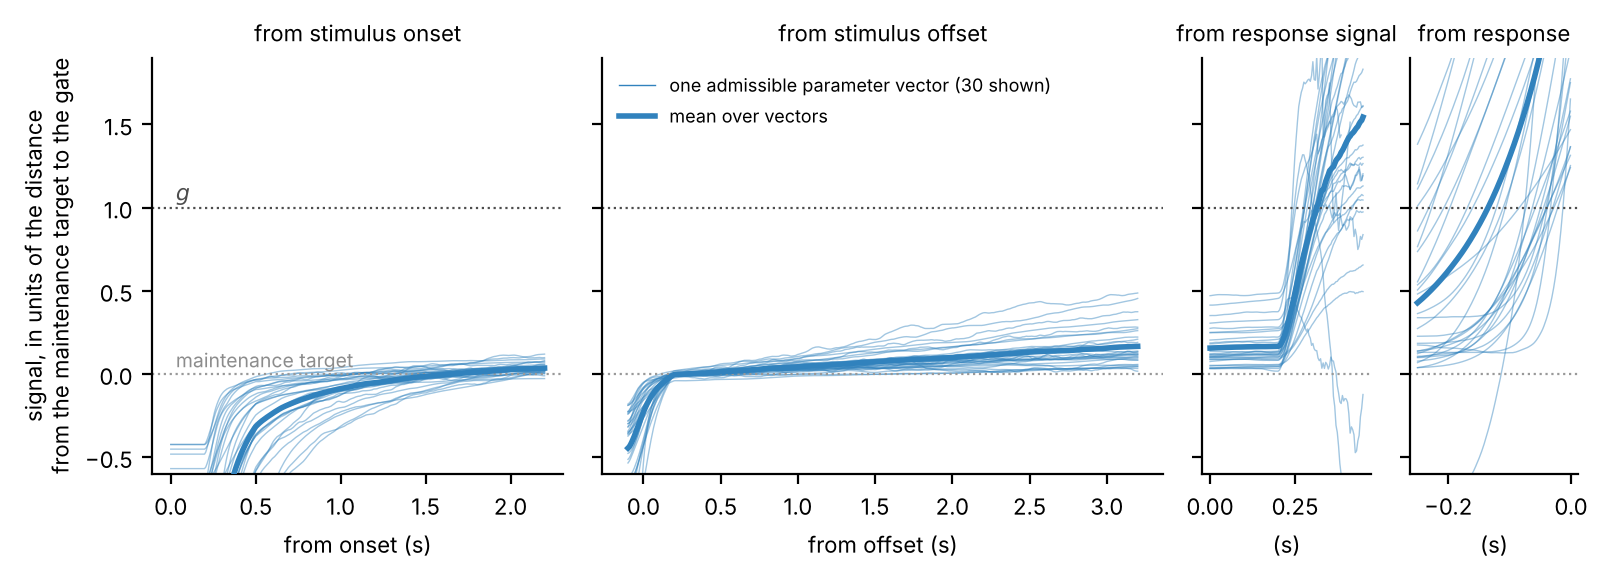
\includegraphics[width=\linewidth]{figures/fig01.png}\end{center}

\begin{center}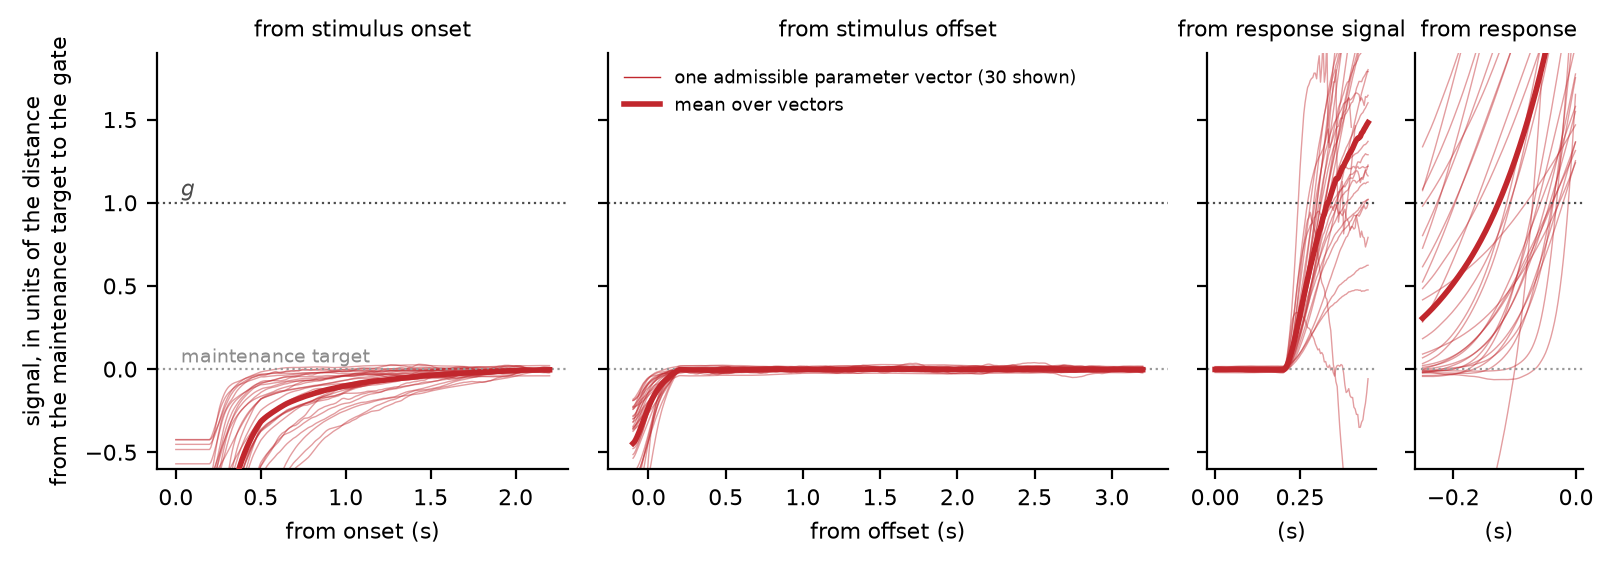
\includegraphics[width=\linewidth]{figures/fig02.png}\end{center}

\captionof{figure}{\textbf{Simulated dynamics under the two candidate models.} The gated motor-preparatory signal, time-locked to the four trial events (stimulus onset, stimulus offset, response signal, response); each trial is censored at its own response. Each thin line is the mean over trials of one admissible parameter set, and the thick line the mean over sets; thirty sets are shown, the same ones in both panels, so that the two panels differ in $\beta$ and in nothing else. The vertical axis is in units of each set's own distance from the maintained level to the gate, so that sets with different amplitudes are superimposable: 0 is the maintained level and the dotted line at 1 is the gate $g$. Top: Model 2 (maintained evidence-dependent state plus temporal preparation). Bottom: Model 1 (maintained evidence-dependent state only), the same sets with $\beta =0$. The two models differ only during the delay period, where Model 2 climbs toward the gate as the response signal approaches and Model 1 does not move at all, at every one of the thirty settings (Corollary~\ref{cor:flat}). Compare Fig~\ref{fig:design}B, one simulated trial.}\label{fig:dynamics}

\begin{center}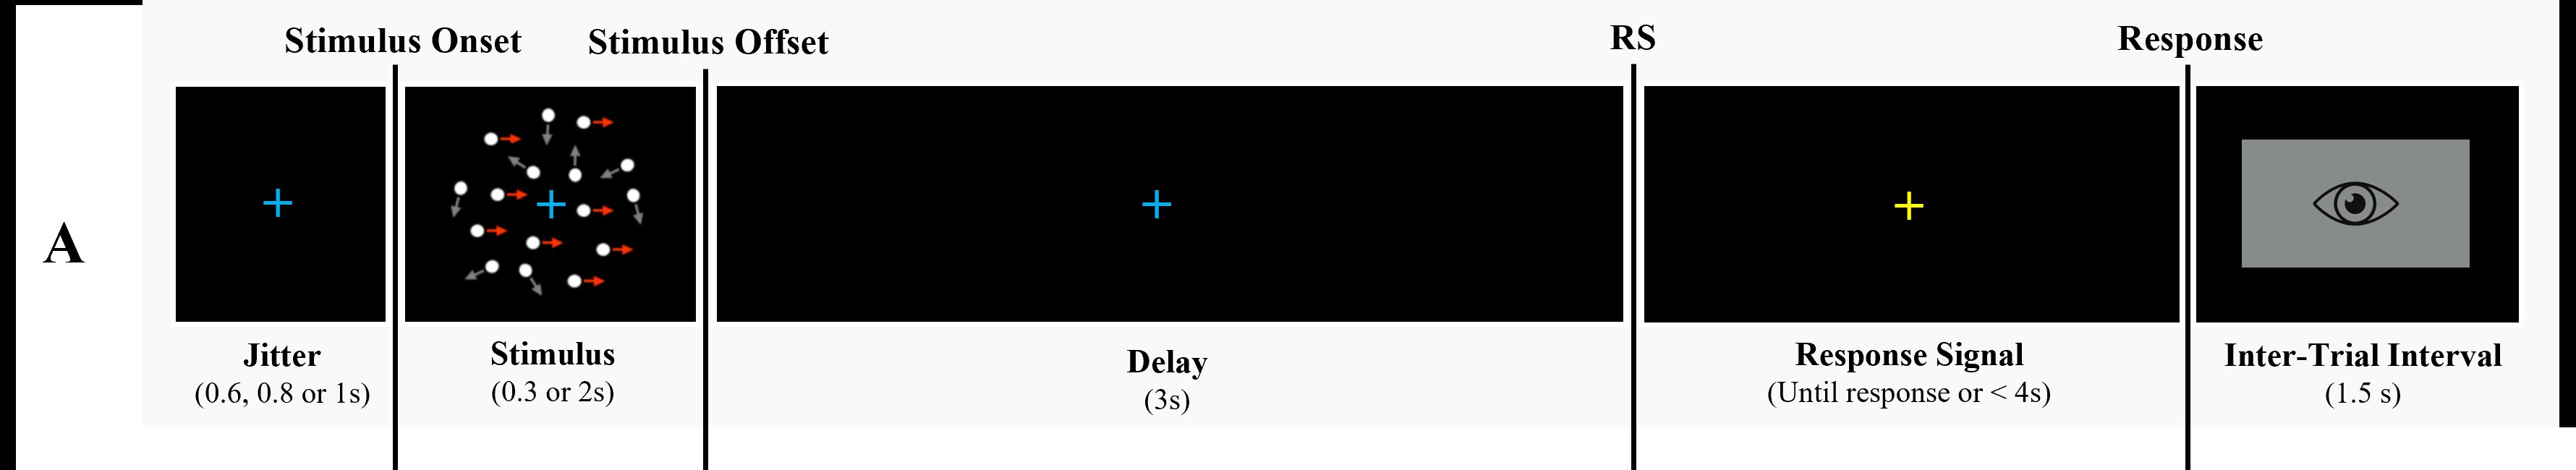
\includegraphics[width=\linewidth]{figures/fig03.png}\end{center}

\begin{center}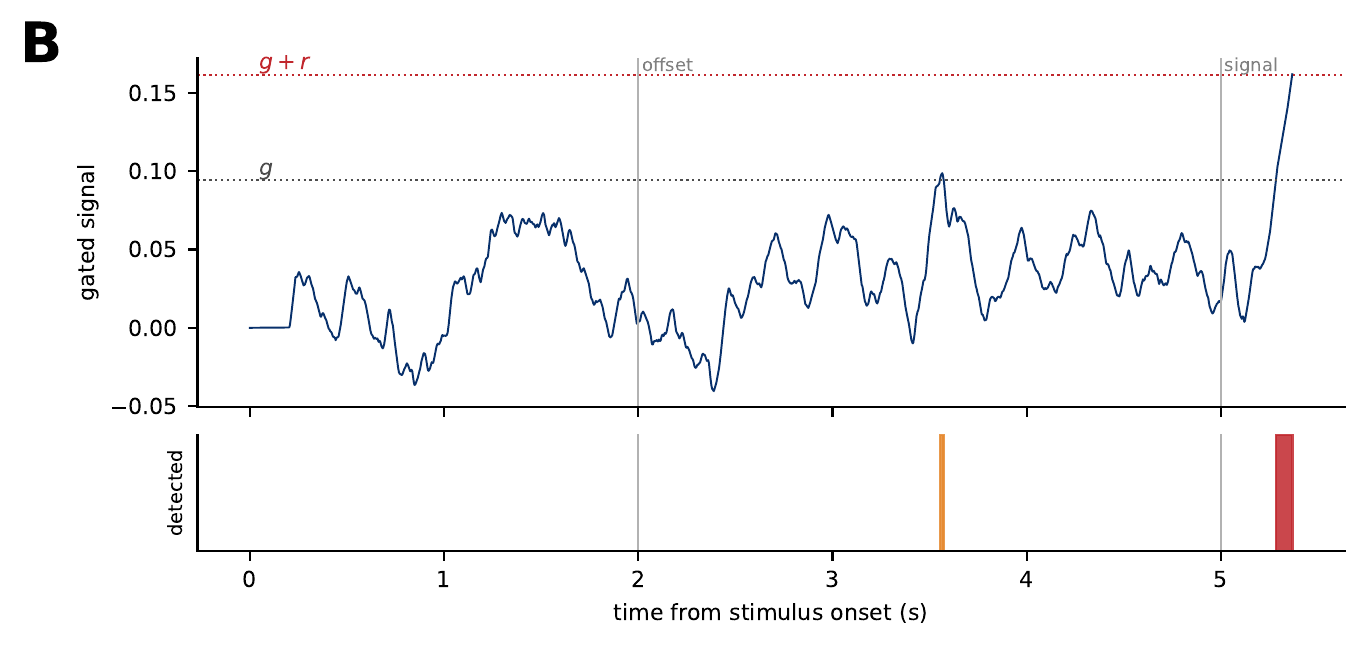
\includegraphics[width=\linewidth]{figures/fig04.png}\end{center}

\captionof{figure}{\textbf{Experimental design and single-trial theoretical dynamics at the motor preparation and muscle activation levels}\textbf{.}  Panel A illustrates the time-course of a trial in our response signal (RS) variant of the random-dot motion task. See text for details.   Muscle activation begins when motor preparation exceeds gating inhibition (parameter \emph{g}). The response time (RT) corresponds to the latency between RS onset and the response. In the present study, it is decomposed into a pre-motor execution time (PMET) and a motor execution time (MET), based on the onset of muscle activation leading up to the response.   Panel B shows one simulated trial from Model 2, at the representative admissible parameter vector (Materials and Methods), the single-trial counterpart of the mean trajectories in Fig~\ref{fig:dynamics}. Above, the gated signal reaching the response effector, with the gate g and the response criterion g+r; below, the activation intervals returned by the same detection procedure applied to the EMG data (see Materials and Methods), after merging intervals within 25 ms and discarding intervals with too few supra-threshold samples. Orange marks a partial muscle activation; red marks the activation that reaches the criterion and becomes the overt response.}\label{fig:design}

\begin{center}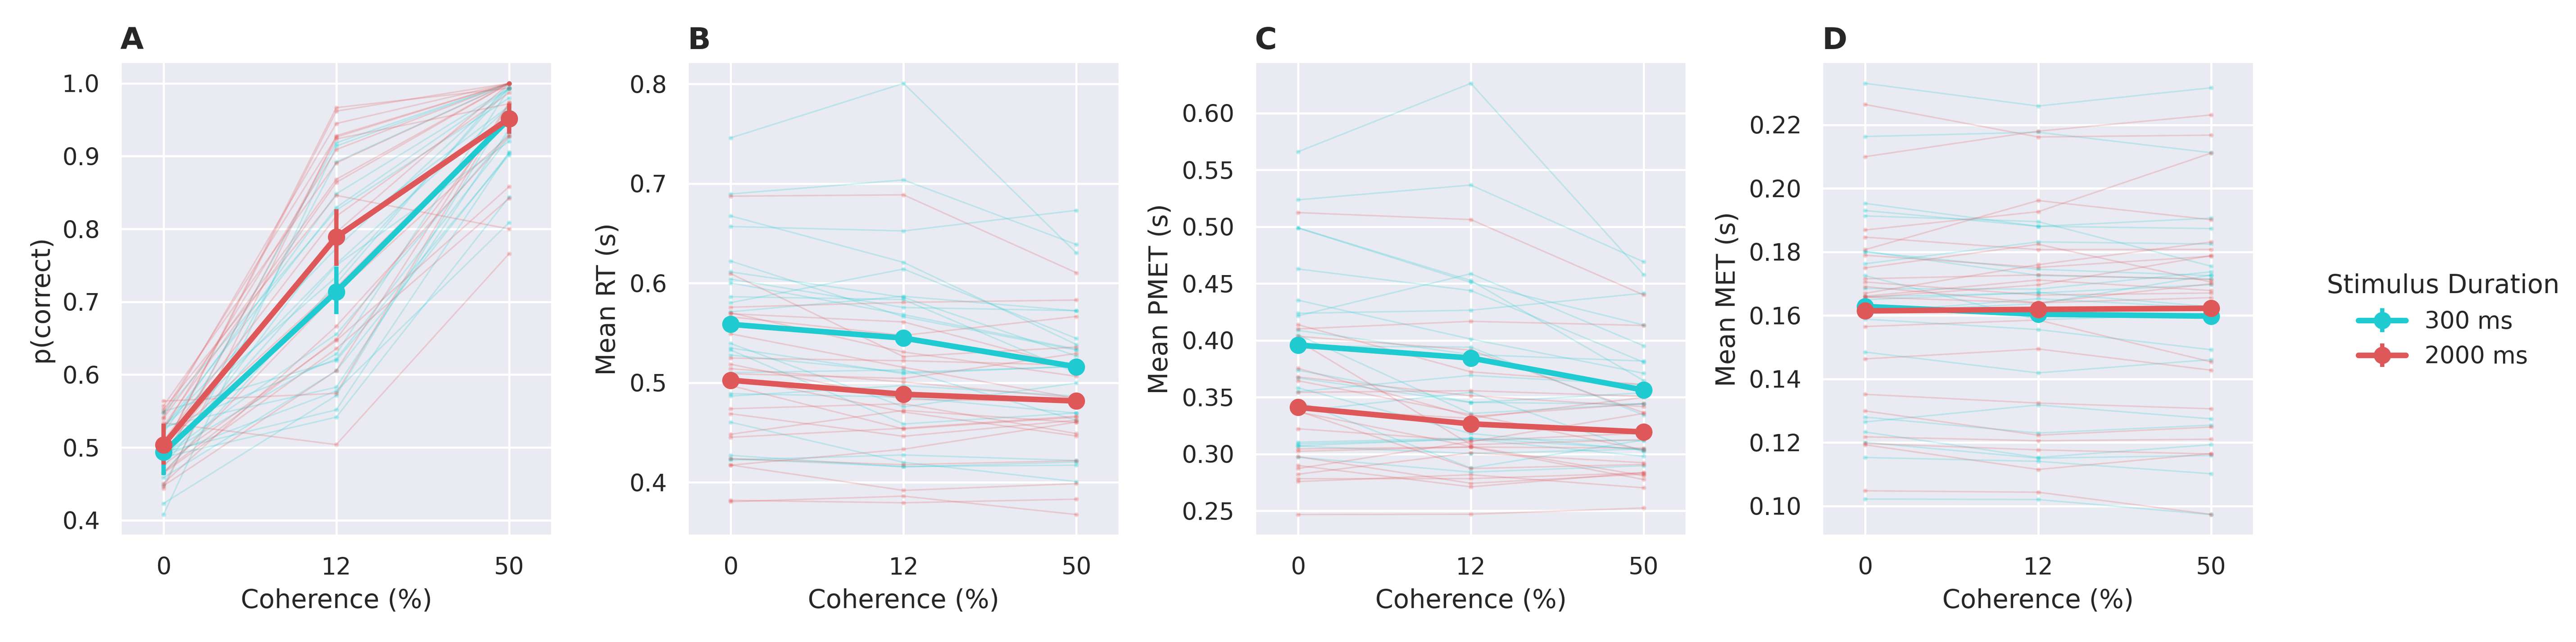
\includegraphics[width=\linewidth]{figures/fig05.png}\end{center}

\captionof{figure}{Behavioral outcomes and response time fractionation based on the onset of muscle activation preceding the response. Panels A-D show, respectively, response accuracy, mean response time (RT), mean pre-motor execution time (PMET), and mean motor execution time (MET) as a function of motion coherence and duration. Faint lines show individual participants. Error bars represent a within-subjects interval about the mean, computed on Cousineau--Morey-normalized values \parencite{moreyConfidenceIntervalsNormalized2008} in every panel: $\pm$1 within-subjects SEM for RT, PMET, and MET, and, for accuracy, a 95\% percentile bootstrap interval over the normalized values (10,000 resamples over participants, Morey-scaled), which is asymmetric where the data approach the [0, 1] bounds and for which a symmetric SEM would not be appropriate.  s = seconds.}\label{fig:behavior}

\begin{center}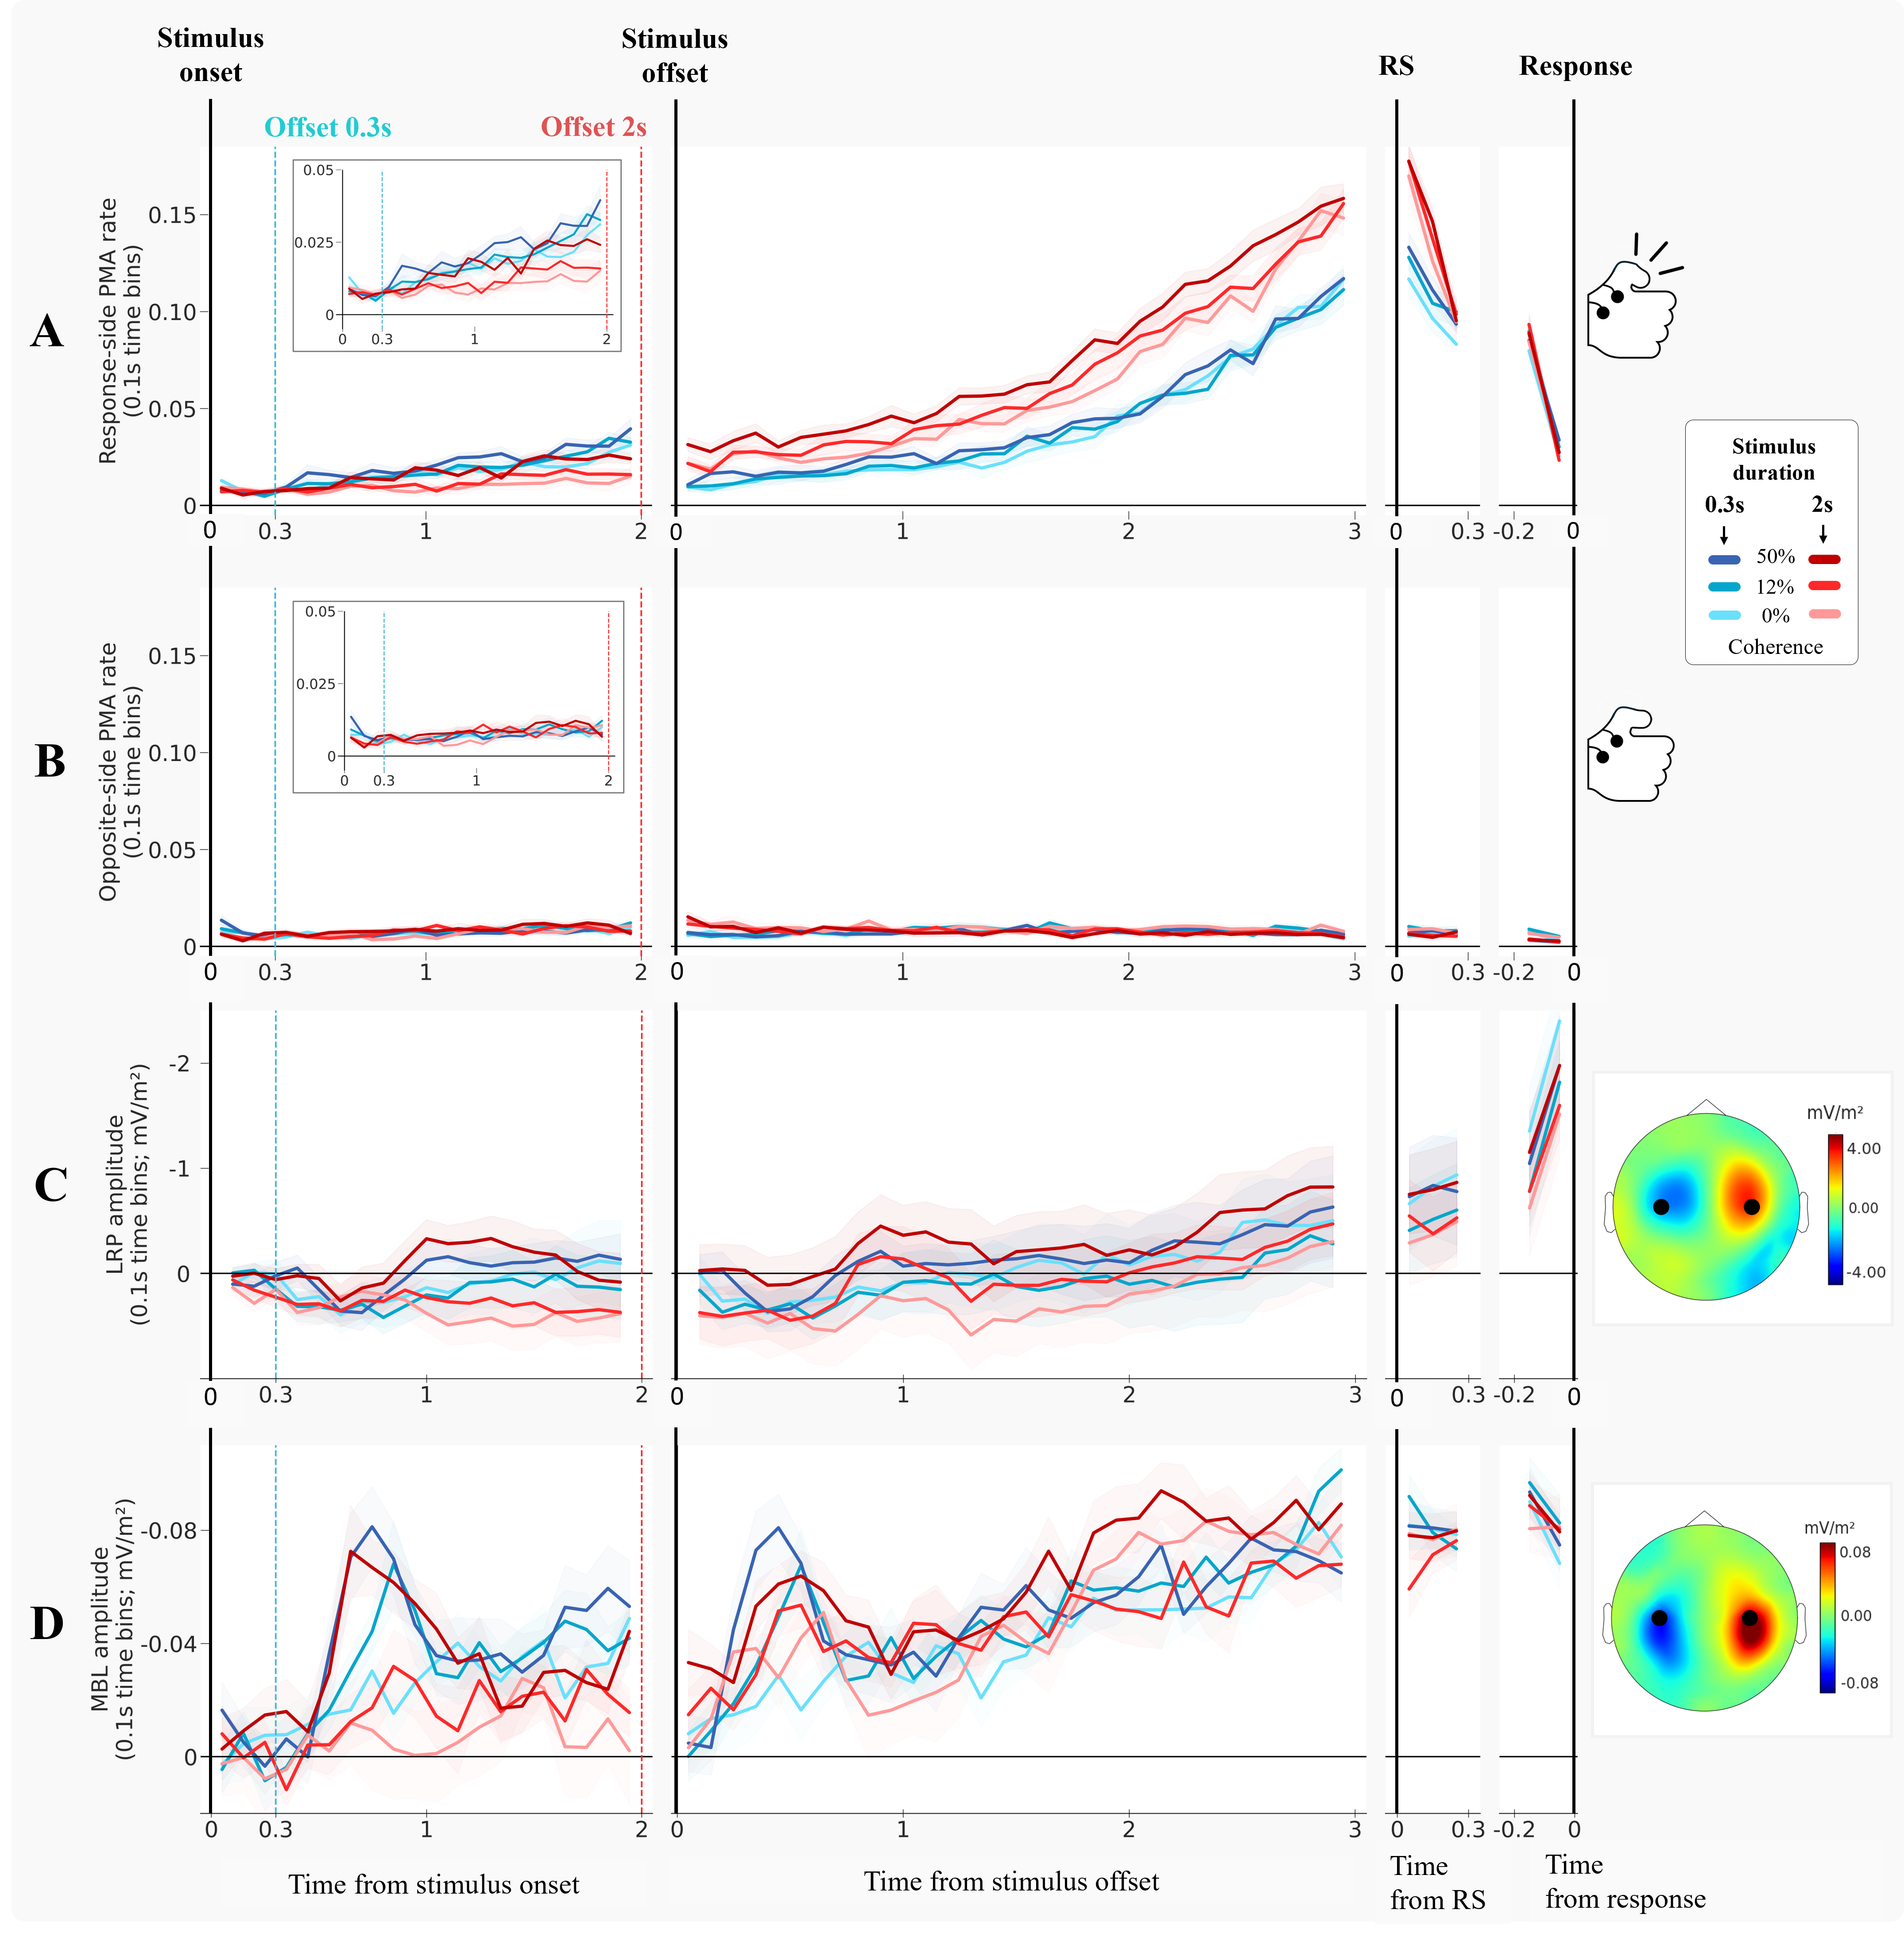
\includegraphics[width=\linewidth]{figures/fig06.png}\end{center}

\captionof{figure}{\textbf{Rate of partial muscle activations and electroencephalographic measures of effector-selective motor preparation aligned to each trial event}\textbf{.}  A) Grand-average rate of partial muscle activations (PMAs) in the electromyographic channel of the responding effector as a function of motion coherence and duration. PMA rate was estimated as the mean number of PMAs per 0.1-s bin.  From left to right, subplots show PMA rate aligned to stimulus onset, stimulus offset, RS onset, and the response, respectively. These locking events are indicated by the black vertical lines. The inset in the leftmost subplot provides a zoomed view of the corresponding data. The grand-average rate of PMAs in the opposite electromyographic channel is shown in panel B. C) Grand-average lateralized readiness potential (LRP)  computed in 0.1 s bins, as a function of motion coherence and duration. The layout of the subplots matches that of panels A and B.  The y-axis is inverted such that upward deflections indicate stronger effector-selective motor preparation. The map on the right shows the grand-average scalp topography in the -0.2 to 0 s interval relative to the response, collapsed across experimental conditions. It was computed by subtracting the mean current source density amplitude for right-hand trials from that for left-hand trials. Black circles indicate the electrode sites used to compute the LRP (C3 and C4). D) Grand-average mu--beta-band spectral amplitude lateralization (MBL), computed in 0.1 s bins, as a function of motion coherence and duration. The y-axis is also inverted such that upward deflections indicate stronger effector-selective motor preparation.  The layout of the subplots matches that of the other panels.  The map on the right shows the grand-average scalp topography in the -0.2 to 0 s interval relative to the response, collapsed across experimental conditions. It was computed by subtracting the mean mu--beta-band spectral amplitude for right-hand trials from that for left-hand trials. For all panels, shaded areas represent $\pm$1 within-subjects standard error of the mean, computed using the method proposed by \textcite{moreyConfidenceIntervalsNormalized2008}.  s = seconds; mV/m\textsuperscript{2} = millivolts per square meter.}\label{fig:pmaeeg}

\begin{center}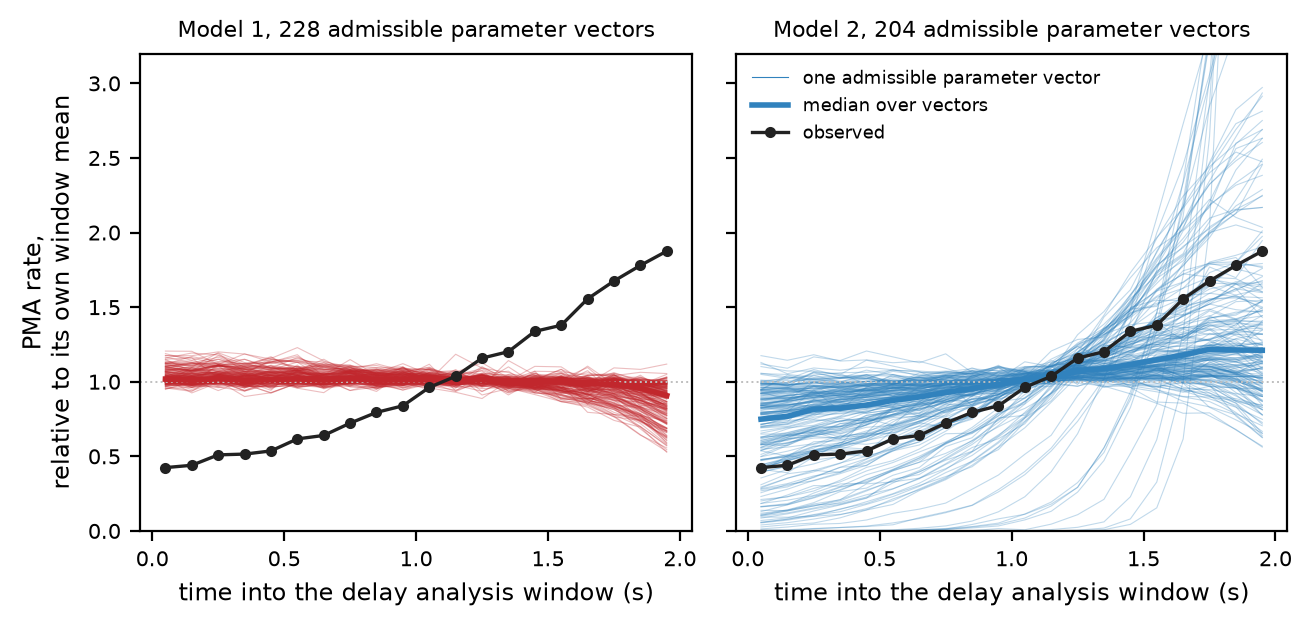
\includegraphics[width=\linewidth]{figures/fig07.png}\end{center}

\captionof{figure}{\textbf{The shape of the delay-period rate curve, one line per admissible draw.} Each thin line is the delay-period profile of one admissible draw divided by its own mean over the window, so that draws whose rates differ by two orders of magnitude are comparable on shape; the thick line is the median over draws and the black points the observed profile, normalised the same way. Every admissible draw of Model 1 is flat, as Corollary~\ref{cor:flat} requires; Model 2's fan out, many of them tracking the observed rise and beyond.}\label{fig:shape}

\begin{center}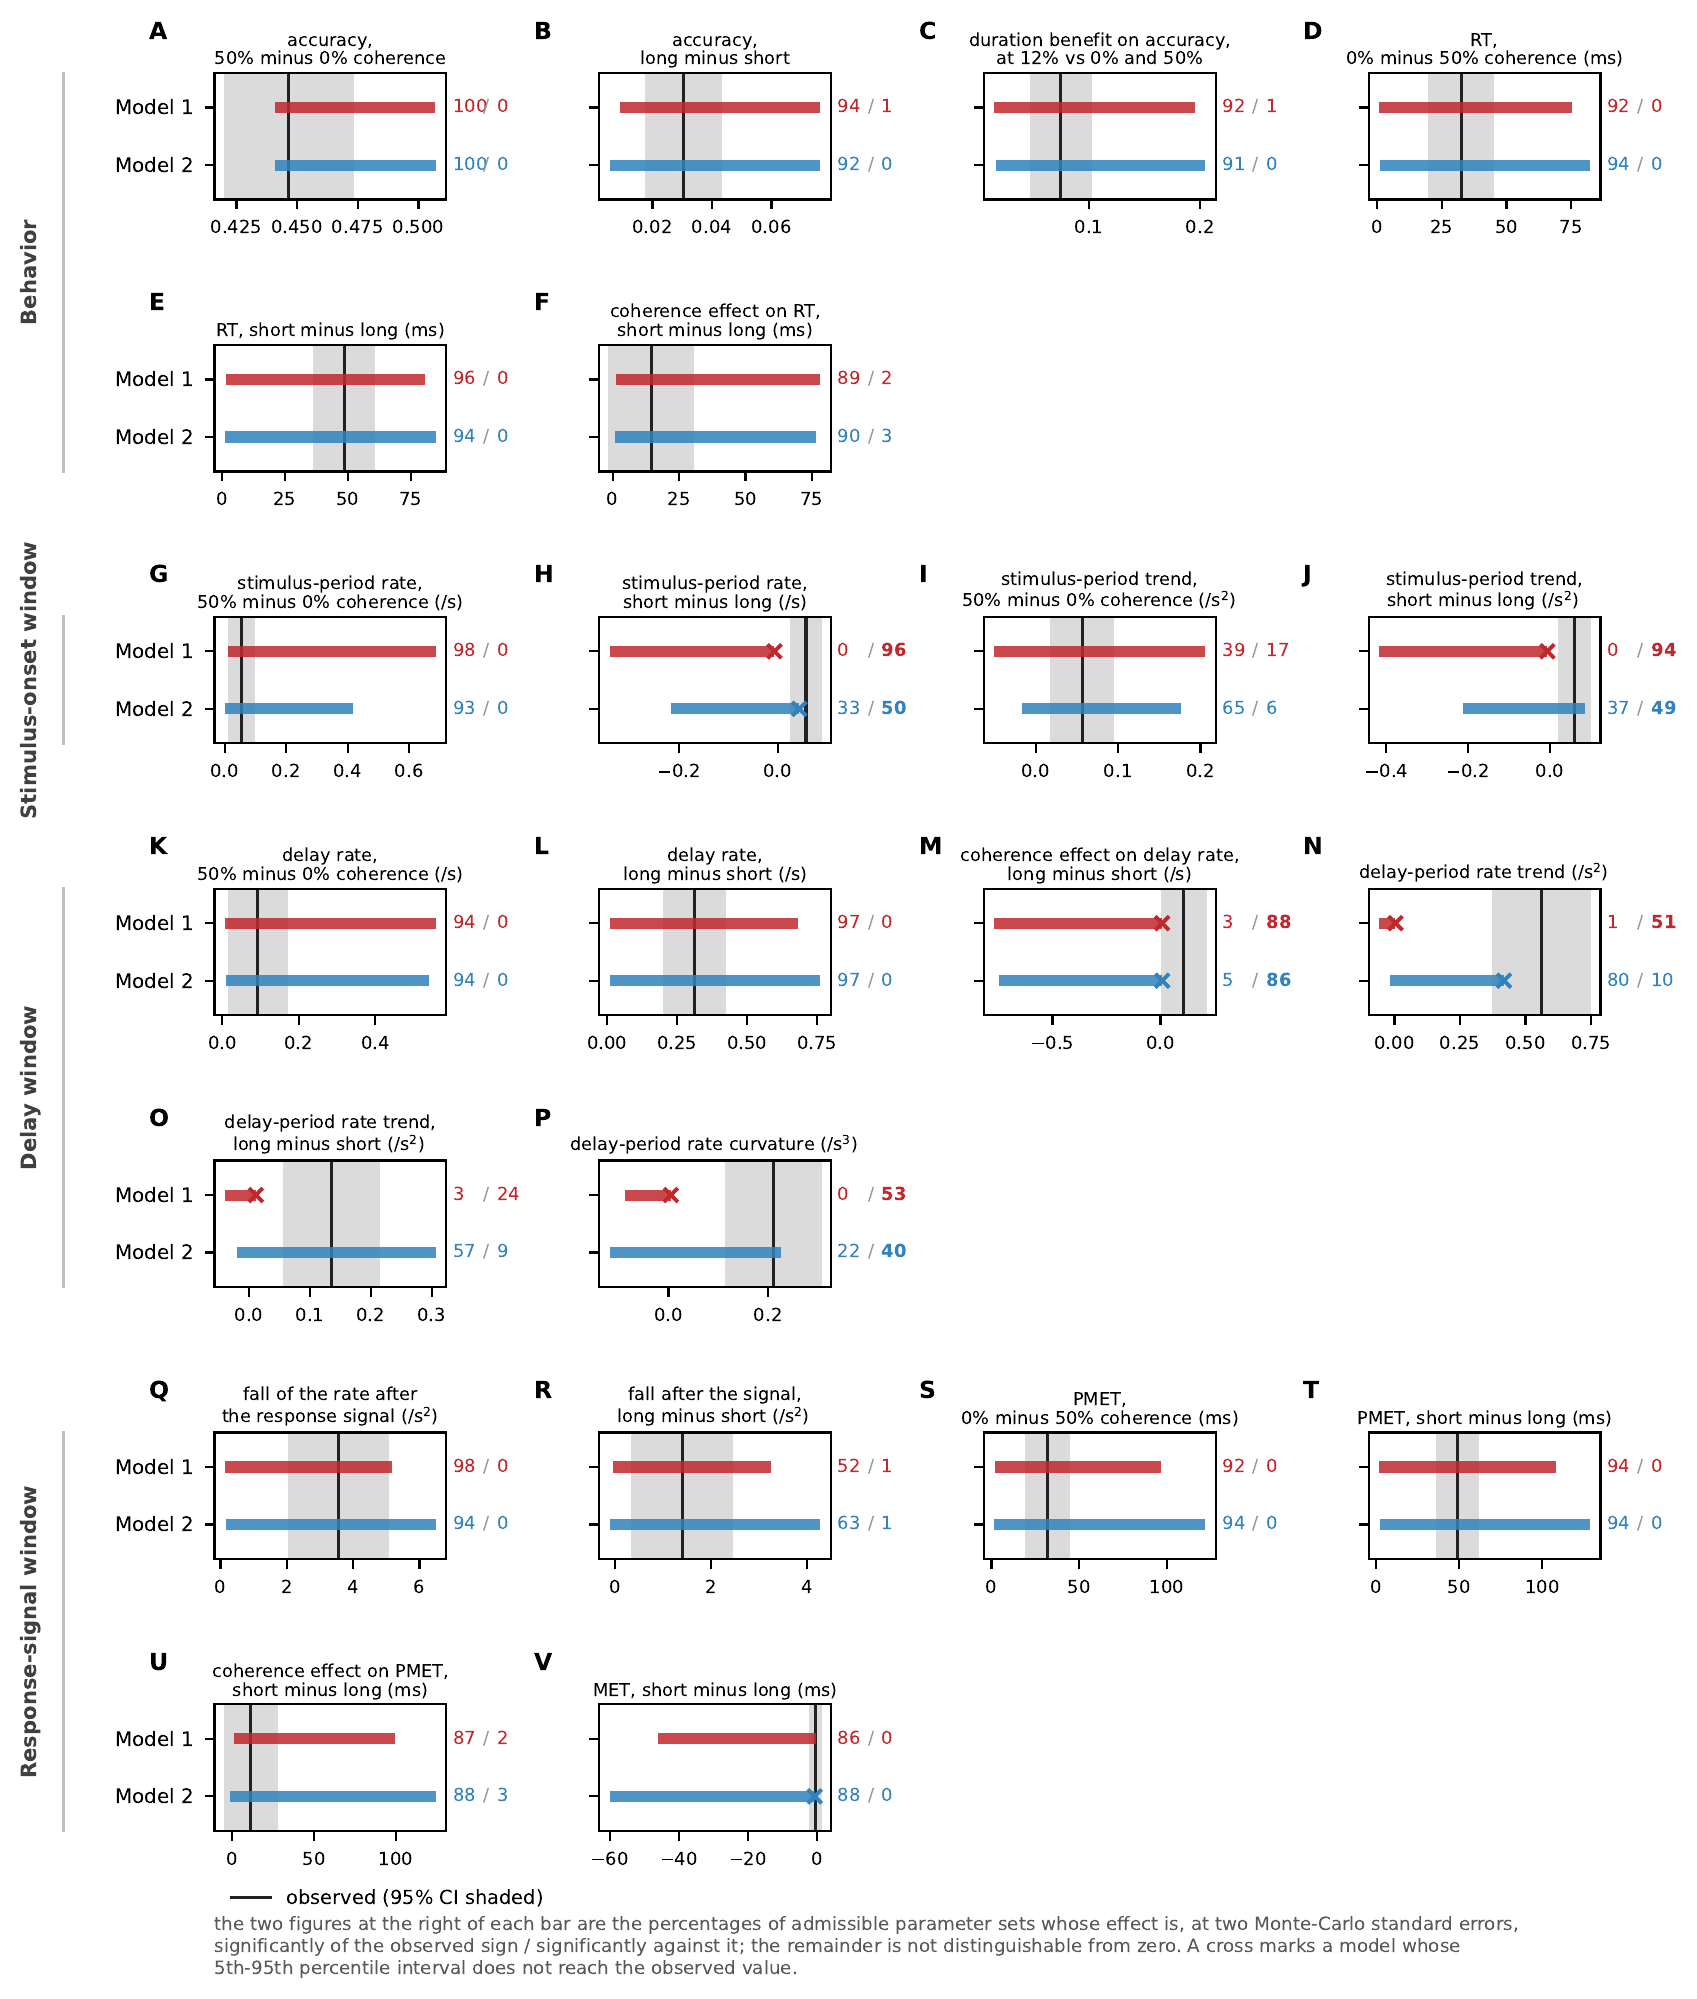
\includegraphics[width=\linewidth]{figures/fig08.png}\end{center}

\captionof{figure}{\textbf{Effect sizes each model can produce, against the observed value, for every effect on behavior or partial-activation rate that the Results report.} Panels are grouped by analysis window, named down the left margin, in the order the Results take them. \textbf{A--F}, behavior: coherence, duration and their interaction on accuracy, then on response time. \textbf{G--J}, stimulus-onset window: coherence and duration effects on the level of the partial-activation rate, then the same two on its linear trend. \textbf{K--P}, delay window: coherence, duration and their interaction on the level, then the trend, the duration effect on the trend, and the curvature. \textbf{Q--V}, response-signal window: the fall of the rate after the signal and its duration-dependence, then coherence, duration and their interaction on premotor execution time, and the duration effect on motor execution time. Each effect is written so that the sign the derivation predicts is positive, and the panel title says which difference is taken. Bars span the 5th to 95th percentile of the effect over each model's admissible draws; the vertical line is the observed value and the grey band its 95\% confidence interval across participants; a cross marks a bar that does not reach the observed value. The two figures at the right of each bar are the percentages of admissible sets whose effect is, at two Monte-Carlo standard errors, significantly of the observed sign and significantly against it; the remainder is not distinguishable from zero. Three classes of reported effect are absent: the electroencephalographic measures, for which the models predict a direction but no magnitude; a few interactions that are null in the data and in both models; and the response window, together with the level of the rate in the response-signal window, where the simulation and the data do not measure the same thing (Results). Contrasts within the response-signal window are unaffected and are shown.}\label{fig:effects}

\begin{center}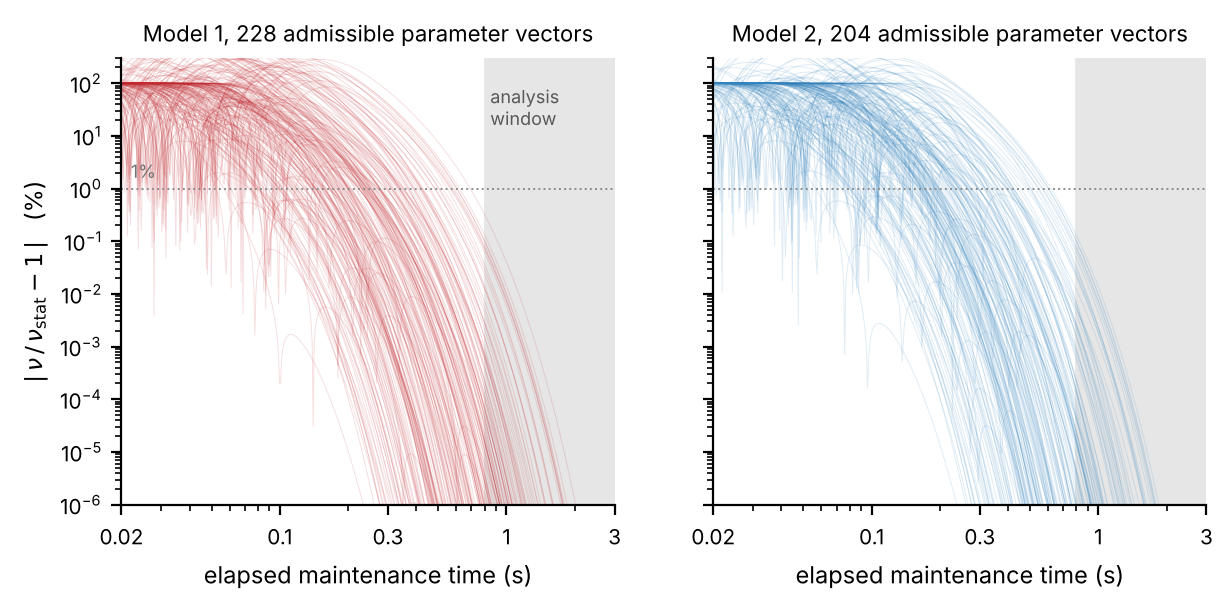
\includegraphics[width=\linewidth]{figures/fig09.png}\end{center}

\captionof{figure}{\textbf{Error of the stationary approximation, over the admissible draws.} Each thin line is one admissible parameter vector: the relative difference between the exact partial-activation rate, Equation~\eqref{eq:nu2} with the transient moments of Equation~\eqref{eq:moments}, and its stationary form, Equation~\eqref{eq:nu_asymp}, as a function of elapsed maintenance time. Both axes are logarithmic and the shaded band is the delay analysis window, which begins at least 1 s after maintenance onset. Left, Model 1; right, Model 2, restricted to the vectors at which temporal preparation does not carry the signal past the gate within the window. Inside the window the largest departure is $6.8\times10^{-3}$\%. Admissible draws only: over the whole sampled box the departure reaches a per cent, on vectors whose rate is far too small to be measured (Appendix, Corollary~\ref{cor:approx}).}\label{fig:approx}


\section{Tables}

\captionof{table}{Variables and parameters of the extended evidence-accumulation model for delayed reports.}\label{tab:params}

\begin{center}\small
\begin{tabular}{>{\raggedright\arraybackslash}p{0.095\linewidth}>{\raggedright\arraybackslash}p{0.541\linewidth}>{\raggedright\arraybackslash}p{0.294\linewidth}}
\toprule
Symbol & Description & Value or range used in simulations (if applicable) \\ \midrule
\emph{t} & Time measured from motion-stimulus onset & -- \\
\emph{x(t)} & Accumulated motion evidence & See Equation~\eqref{eq:x} \\
$L_{\mathrm{motion}}$ & Motion-evidence  encoding  latency & 0.200 s \\
\emph{s} & Motion direction & $-$1 or +1 \\
\emph{c} & Motion coherence & 0, 0.12, or 0.50 \\
\emph{k} & Scaling of motion coherence into the mean rate of motion-evidence accumulation & 0.5--2.0 (log-uniform); \textcite{dendauwGatedCascadeDiffusion2024} estimate 1.183 \\
$\sigma_{x}$ & Diffusion coefficient of motion-evidence accumulation & 0.100 \\
\emph{y(t)} & Filtered  motor-preparatory state & See Equations~\eqref{eq:y}, \eqref{eq:y_delay} and \eqref{eq:y_RS} \\
\emph{$\lambda$} & Gain of the low-pass filter relating decision-related input to motor preparation & 10--50 s\textsuperscript{-1} (log-uniform); \textcite{dendauwGatedCascadeDiffusion2024} estimate 21.471 \\
$z_{L}(t)$, $z_{R}(t)$ & Neural drives to the left and right response agonists & See Equation~\eqref{eq:z} \\
\emph{g} & Level of gating inhibition & 0.050--0.200 \\
\emph{r} & Response criterion applied to the neural drive & 0.010--0.200 (log-uniform) \\
$L_{\mathrm{motor}}$ & Residual motor latency between response triggering and the overt response & 0.093 s (fixed; Dendauw et al. 2024) \\
\emph{D} & Motion duration & 0.300 or 2.000 s \\
\emph{$\theta$} & Internal motor-preparation threshold triggering maintenance & \emph{$\theta$/g}  sampled  from 0.25--0.90 \\
\emph{$\tau$} & Maintenance-onset time & Trial-dependent \\
\emph{m} & Maintenance target & See Equation~\eqref{eq:m} \\
$s_{\mathrm{resp}}$ & Selected  response direction & $-$1: left; +1: right \\
\emph{$\varepsilon$(t)} & Stochastic fluctuations around the maintenance target & See Equation~\eqref{eq:epsilon} \\
\emph{H(t)} & Fluctuation of the motor-preparatory signal about the maintained level & See Equation~\eqref{eq:Hdef} \\
\emph{$\kappa$} & Mean-reversion rate of maintenance fluctuations & 0.20--30.0 s\textsuperscript{-1} (log-uniform) \\
$\sigma_{\varepsilon}$ & Diffusion coefficient of maintenance fluctuations & = ${\mathrm{SD}}_{\varepsilon }\sqrt{2\kappa }$, with ${\mathrm{SD}}_{\varepsilon }$ 0.003--0.060 (log-uniform) \\
$t_{\mathrm{offset}}$ & Time at which stimulus offset becomes internally available as a temporal reference & \emph{D} + $L_{\mathrm{motion}}$ \\
$L_{\mathrm{RS}}$ & RS-evidence  encoding  latency & 0.200 s \\
$t_{\mathrm{RS}}$ & Time at which RS evidence becomes available to the accumulation process & \emph{D} + 3 + $L_{\mathrm{RS}}$ \\
\emph{$\beta$} & Maximum additive contribution of temporal preparation to the motor-preparatory signal reaching the downstream gate & Model 1: 0; Model 2: 0.0015--0.100 (log-uniform) \\
\emph{q(t)} & Accumulated evidence that the RS is present & See Equation~\eqref{eq:q} \\
$\mu_{\mathrm{RS}}$ & Mean rate of RS-evidence accumulation & 0.30--1.50 \\
$\sigma_{q}$ & Diffusion coefficient of RS-evidence accumulation & 0.03--0.30 (log-uniform) \\
\bottomrule
\end{tabular}
\end{center}
Note. The ranges are those sampled in the parameter-space evaluation, and their provenance is given there (Materials and Methods, Evaluation over the parameter space); entries without a range were held fixed. RS: response signal.



\section{Appendix. The rate of partial muscle activations}

This appendix derives the instantaneous rate at which the maintained motor-preparatory signal crosses the gate upward, which is a partial muscle activation, and the properties of that rate which the Results test.


\subsection{Setup and notation}

Notation follows Theory (Materials and Methods) and Table~\ref{tab:params}; $\varphi$ and $\Phi$ are the standard normal density and distribution function. Fix a trial that has entered maintenance at time $\tau $ with selected response ${s}_{\mathrm{resp}}$ and maintained level $m$ (Equation~\eqref{eq:m}), and write $\rho :=t-\tau $ for elapsed maintenance time. For $t\ge \tau $ let $y\left(t\right)=m+H\left(t\right)$, so that $H$ is the fluctuation of the motor-preparatory signal about the level it maintains. By Equations~\eqref{eq:epsilon} and~\eqref{eq:y_delay},

\begin{eqnarray}
    \dd \varepsilon \left(t\right) &=& -\kappa \varepsilon \left(t\right)\, \dd t+{\sigma }_{\varepsilon }\, \dd {W}_{\varepsilon }\left(t\right), \qquad \varepsilon \left(\tau \right)\sim \mathrm{N}\left(0,{\mathrm{SD}}_{\varepsilon }^{2}\right), \nonumber \\
    \dd H\left(t\right) &= &\lambda \left(\varepsilon \left(t\right)-H\left(t\right)\right)\, \dd t
\label{eq:H}
\end{eqnarray}


with ${\sigma }_{\varepsilon }={\mathrm{SD}}_{\varepsilon }\sqrt{2\kappa }$, so that ${\mathrm{SD}}_{\varepsilon }^{2}$ is the stationary variance of $\varepsilon$ and the maintenance noise begins in its own stationary state, independently of ${W}_{\varepsilon }$ and of the motion-evidence noise. By construction $H\left(\tau \right)=0$, since the filter output is continuous and $m$ is its value at $\tau $.

Since $\varepsilon$ is symmetric and independent of the sign of the response, ${s}_{\mathrm{resp}}H$ has the same law as $H$. Writing $\delta :={t}_{\mathrm{RS}}-{t}_{\mathrm{offset}}$ for the length of the preparation window and $d(t)$ for the distance from the maintained level to the gate,

\begin{equation}
d\left(t\right)=g-\left|m\right|-\frac{\beta }{\delta }{\left(t-{t}_{\mathrm{offset}}\right)}^{+}
\label{eq:d}
\end{equation}


(the second term present only under temporal preparation, so that $\beta =0$ under Model 1), a partial activation on the selected channel begins exactly when ${s}_{\mathrm{resp}}H$ crosses $d\left(t\right)$ upward. Temporal preparation therefore carries the signal toward the gate at the constant speed $\beta /\delta$. The non-selected channel activates when ${s}_{\mathrm{resp}}H$ falls below $-\left(g+\left|m\right|+\frac{\beta }{\delta }{\left(t-{t}_{\mathrm{offset}}\right)}^{+}\right)$. Since ${s}_{\mathrm{resp}}H$ has the same law as $-{s}_{\mathrm{resp}}H$, its rate is that of the selected channel with $d\left(t\right)$ replaced by this distance, which is larger than $d\left(t\right)$ by $2\left|m\right|+2\frac{\beta }{\delta }{\left(t-{t}_{\mathrm{offset}}\right)}^{+}$, and with the barrier moving away rather than toward the signal. In the stationary regime established below, its rate is therefore at most that of the selected channel, with equality only when $m=0$ and $\beta =0$; under Model 1 the ratio of the two rates is ${e}^{-2g\left|m\right|/{\sigma }_{H}^{2}}$. It is not considered further.

\subsection{The maintained fluctuation}

Solving Equation~\eqref{eq:H} gives

\begin{eqnarray*}
    \varepsilon \left(\tau +\rho \right)&=&\varepsilon \left(\tau \right){e}^{-\kappa \rho }+{\sigma }_{\varepsilon }\int_{0}^{\rho } {e}^{-\kappa \left(\rho -p\right)}\,\dd {W}_{\varepsilon }\left(p\right),\\ H\left(\tau +\rho \right)&=&\lambda \int_{0}^{\rho } {e}^{-\lambda \left(\rho -q\right)}\varepsilon \left(\tau +q\right)\, \dd q
\end{eqnarray*}


Since $\varepsilon$ admits a continuous modification and $H$ is then a Riemann integral of a continuous function, almost surely $H\in {C}^{1}$. Substituting the first line into the second and exchanging the order of integration (permissible because the integrand is bounded on $\{0\le p\le q\le \rho \}$) gives

\begin{eqnarray*}
    H\left(\tau +\rho \right)&=&\frac{\varepsilon \left(\tau \right)}{{\sigma }_{\varepsilon }}K\left(\rho \right)+\int_{0}^{\rho } K\left(\rho -p\right)\,
    \dd {W}_{\varepsilon }\left(p\right) \\
    K\left(v\right)&=&
    \begin{cases}
        \frac{\lambda {\sigma }_{\varepsilon }}{\lambda -\kappa }\left({e}^{-\kappa v}-{e}^{-\lambda v}\right), & \kappa \neq \lambda, \\
\lambda {\sigma }_{\varepsilon }\,v\,{e}^{-\lambda v}, & \kappa =\lambda.
        \end{cases}
\end{eqnarray*}


$H$ is therefore a centred Gaussian process, being a linear combination of the Gaussian $\varepsilon \left(\tau \right)$ and an independent Wiener integral. Note that $K\left(0\right)=0$, which makes the first term vanish at $\rho =0$ and recovers $H\left(\tau \right)=0$, and that ${K}^{'}\left(0\right)=\lambda {\sigma }_{\varepsilon }$. Differentiating under the integral and using $K\left(0\right)=0$ to kill the boundary term, $\dot{H}\left(\tau +\rho \right)=\left(\varepsilon \left(\tau \right)/{\sigma }_{\varepsilon }\right){K}^{'}\left(\rho \right)+\int_{0}^{\rho } {K}^{'}\left(\rho -p\right)\, \dd {W}_{\varepsilon }\left(p\right)$. Write ${\sigma }_{H}^{2}\left(\rho \right):=\Var H\left(\tau +\rho \right)$, ${\sigma }_{\dot{H}}^{2}\left(\rho \right):=\Var \dot{H}\left(\tau +\rho \right)$ and ${c}_{H}\left(\rho \right):=\Cov \left(H\left(\tau +\rho \right),\dot{H}\left(\tau +\rho \right)\right)$, and the same symbols without an argument for their limits as $\rho \to \infty $. Because $\varepsilon \left(\tau \right)$ and ${W}_{\varepsilon }$ are independent, the It\^o isometry gives each moment as the sum of the two contributions, ${\sigma }_{H}^{2}\left(\rho \right)={K}^{2}\left(\rho \right)/2\kappa +\int_{0}^{\rho } {K}^{2}$, ${\sigma }_{\dot{H}}^{2}\left(\rho \right)={K}^{'2}\left(\rho \right)/2\kappa +\int_{0}^{\rho } {K}^{'2}$ and ${c}_{H}\left(\rho \right)=K\left(\rho \right){K}^{'}\left(\rho \right)/2\kappa +{K}^{2}\left(\rho \right)/2$. Evaluating them, and writing  ${E}_{1}\left(\rho \right):={e}^{-\left(\lambda +\kappa \right)\rho }$, ${E}_{2}\left(\rho \right):={e}^{-2\lambda \rho }$, with  $X\left(\rho \right):=\frac{\lambda +\kappa }{\lambda -\kappa }\left({E}_{2}\left(\rho \right)-{E}_{1}\left(\rho \right)\right)$ if $\kappa \neq \lambda$ and $X\left(\rho \right)=-2\lambda \rho {E}_{2}\left(\rho \right)$ if $\kappa = \lambda$, the three moments are

  \begin{equation}\label{eq:moments}
\begin{aligned}
\sigma_H^2(\rho) &= \sigma_H^2\bigl(1+X(\rho)-E_1(\rho)\bigr)\\
c_H(\rho) &= -\lambda\,\sigma_H^2\,X(\rho)\\
\sigma_{\dot H}^2(\rho)
  &= \sigma_{\dot H}^2\left(1+\frac{\lambda}{\kappa}\bigl(X(\rho)+E_1(\rho)\bigr)\right)
\end{aligned}
\end{equation}


where the stationary limits, reached as $\rho \to \infty $ since ${E}_{1}\left(\rho \right),{E}_{2}\left(\rho \right)\to 0$, are

\begin{equation}\label{eq:asymp_moments}
{\sigma }_{H}^{2} = \frac{\lambda \, {\mathrm{SD}}_{\varepsilon }^{2}}{\lambda +\kappa }, \quad {\sigma }_{\dot{H}}^{2}= \frac{{\lambda }^{2}\kappa \, {\mathrm{SD}}_{\varepsilon }^{2}}{\lambda +\kappa }, \quad {c}_{H} = 0.
\end{equation}


Setting $\rho =0$ in Equation~\eqref{eq:moments} gives ${\sigma }_{H}^{2}\left(0\right)=0$ and ${\sigma }_{\dot{H}}^{2}\left(0\right)={\lambda }^{2}{\mathrm{SD}}_{\varepsilon }^{2}$: the fluctuation of the signal about the maintained level starts at zero and fills in, while its derivative starts above its stationary value and falls. Temporal preparation is added outside the filter (Equation~\eqref{eq:tildey}), so it shifts the mean of the gate-facing signal and leaves all three moments untouched; Equations~\eqref{eq:moments} and~\eqref{eq:asymp_moments} hold for both models.

\begin{proposition}[the analysis window lies in the stationary regime]\label{prop:stationary}
Let $\rho \ge 0.8$ s. Then, over the ranges of Table~\ref{tab:params}, ${E}_{1}\left(\rho \right)<3\times {10}^{-4}$ and $\left|X\left(\rho \right)\right|<2.4\times {10}^{-3}$, whatever $\kappa$. The transient terms of Equation~\eqref{eq:moments} are therefore negligible on the delay analysis window, and the three moments may be replaced there by their stationary values, Equation~\eqref{eq:asymp_moments}.
\end{proposition}


\begin{proof}
Time enters Equation~\eqref{eq:moments} through ${E}_{1}\left(\rho \right)$, ${E}_{2}\left(\rho \right)$ and $X\left(\rho \right)$, and through nothing else. The first two decay at the rates $\lambda +\kappa $ and $2\lambda $, both at least

\begin{equation*}
\mu :=\lambda +\min \left(\lambda ,\kappa \right)\ge \lambda ,
\end{equation*}


and so does the third: applying the mean value theorem to $z\mapsto {e}^{-z\rho }$ between $z=\lambda +\kappa $ and $z=2\lambda $ gives $\left|{E}_{2}\left(\rho \right)-{E}_{1}\left(\rho \right)\right|\le \left|\lambda -\kappa \right|\rho {e}^{-\mu \rho }$, whence $\left|X\left(\rho \right)\right|\le \left(\lambda +\kappa \right)\rho {e}^{-\mu \rho }$. Over the sampled ranges both bounds are largest at $\rho =0.8$ s, $\lambda =10$ s\textsuperscript{-1} and $\kappa =0.2$ s\textsuperscript{-1}, where ${E}_{1}\left(\rho \right)\le {e}^{-8.16}<3\times {10}^{-4}$ and $\left|X\left(\rho \right)\right|\le 8.16\, {e}^{-8.16}<2.4\times {10}^{-3}$.
\end{proof}


Every mode of the transient therefore decays at least as fast as the filter gain $\lambda$, whatever $\kappa$ is: $\kappa$ appears in $\mu$, but only in the direction that makes the decay faster, since $\mu$ increases with $\kappa$ up to $2\lambda $. Maintenance begins no later than ${t}_{\mathrm{offset}}={L}_{\mathrm{motion}}+D$ and the delay analysis window opens 1 s after the physical stimulus offset $D$, so $\rho \ge 1-{L}_{\mathrm{motion}}=0.8$ s throughout that window at every parameter setting sampled, and every statement below is made at the stationary moments.

\subsection{The crossing rate}

Throughout this subsection the distance to the gate is a function of $t$ and the moments of Equation~\eqref{eq:moments} are functions of the elapsed maintenance time $\rho =t-\tau $. Let $Z\left(t\right):={s}_{\mathrm{resp}}H\left(t\right)-d\left(t\right)$, so that upcrossings of $d$ by ${s}_{\mathrm{resp}}H$ are upcrossings of zero by $Z$, and $\dot{Z}=\dot{H}+\beta /\delta$. Trajectories that reach the response criterion before the end of the delay are neglected; they are premature responses, excluded from the empirical analysis and held to a small fraction of trials by the admissibility screen. Since $H$ is almost surely continuously differentiable and $\left(Z,\dot{Z}\right)$ is jointly Gaussian and non-degenerate for $\rho >0$, the Kac--Rice formula gives the expected upcrossing rate \parencite[ch. 3]{azaisLevelSetsExtrema2009}:

\begin{equation}
\nu \left(t\right)={p}_{Z\left(t\right)}\left(0\right)\, \mathrm{E}\left[\dot{Z}\left(t\right){1}_{\{\dot{Z}\left(t\right)>0\}} \mid Z\left(t\right)=0\right]
\label{eq:nu}
\end{equation}


Since $H$ is centred, $Z\left(t\right)\sim \mathrm{N}\left(-d\left(t\right),{\sigma }_{H}^{2}\left(\rho \right)\right)$ and ${p}_{Z\left(t\right)}\left(0\right)=\varphi \left(d\left(t\right)/{\sigma }_{H}\left(\rho \right)\right)/{\sigma }_{H}\left(\rho \right)$. Because $\left(Z,\dot{Z}\right)$ is jointly Gaussian, $\dot{Z}$ given $Z=0$ is Gaussian with mean and variance

\begin{equation*}
M\left(t\right)=\frac{\beta }{\delta }+\frac{{c}_{H}\left(\rho \right)}{{\sigma }_{H}^{2}\left(\rho \right)}d\left(t\right), \quad S\left(t\right)={\sigma }_{\dot{H}}^{2}\left(\rho \right)-\frac{{c}_{H}{\left(\rho \right)}^{2}}{{\sigma }_{H}^{2}\left(\rho \right)}
\end{equation*}


and for $\xi \sim \mathrm{N}\left(M,S\right)$ the expected positive part is $\mathrm{E}\left[\xi {1}_{\{\xi >0\}}\right]=M\Phi \left(M/\sqrt{S}\right)+\sqrt{S}\varphi \left(M/\sqrt{S}\right)$. Substituting into Equation~\eqref{eq:nu} gives the rate in general form,

\begin{equation}
\nu \left(t\right)=\frac{\varphi \left(d\left(t\right)/{\sigma }_{H}\left(\rho \right)\right)}{{\sigma }_{H}\left(\rho \right)}\left[M\left(t\right)\Phi \left(\frac{M\left(t\right)}{\sqrt{S\left(t\right)}}\right)+\sqrt{S\left(t\right)}\varphi \left(\frac{M\left(t\right)}{\sqrt{S\left(t\right)}}\right)\right]
\label{eq:nu2}
\end{equation}


Replacing the moments by their stationary values, which Proposition~\ref{prop:stationary} licenses on the analysis window, sets ${c}_{H}=0$ and therefore $M=\beta /\delta $ and $S={\sigma }_{\dot{H}}^{2}$: both are constants, and all the time dependence is carried by the distance to the gate. Writing

\begin{equation*}
a\left(t\right):=\frac{d\left(t\right)}{{\sigma }_{H}}, \quad \omega :=\frac{{\sigma }_{\dot{H}}}{{\sigma }_{H}}=\sqrt{\lambda \kappa }
\end{equation*}


for the distance to the gate in units of the fluctuation and for the characteristic frequency of the fluctuation, Equation~\eqref{eq:nu2} becomes the \emph{stationary rate}

\begin{equation}
\nustat \left(t\right)=\varphi \left(a\left(t\right)\right)\left[\frac{\beta }{\delta {\sigma }_{H}}\Phi \left(\frac{\beta }{\delta {\sigma }_{\dot{H}}}\right)+\omega \varphi \left(\frac{\beta }{\delta {\sigma }_{\dot{H}}}\right)\right]
\label{eq:nu_asymp}
\end{equation}


The bracket does not depend on the distance to the gate, and temporal preparation enters it only through $\beta /\delta$, the speed at which temporal preparation carries the signal toward the gate. The stationary rate is thus a product of two factors: a Gaussian in the standardized distance to the gate, which is where the conditions and the time within the delay act, and a bracket that depends on neither the motion coherence nor its duration.

\begin{corollary}[error of the stationary rate]\label{cor:approx}
Let $t$ be a time in the delay analysis window and $\rho =t-\tau $ the elapsed maintenance time. Write the three moments of Equation~\eqref{eq:moments} in terms of their departures from their stationary values,
\begin{equation*}
{\sigma }_{H}^{2}\left(\rho \right)={\sigma }_{H}^{2}\left(1+u\left(\rho \right)\right), \quad {\sigma }_{\dot{H}}^{2}\left(\rho \right)={\sigma }_{\dot{H}}^{2}\left(1+v\left(\rho \right)\right), \quad {c}_{H}\left(\rho \right)=w\left(\rho \right){\sigma }_{H}{\sigma }_{\dot{H}},
\end{equation*}
so that $u$ and $v$ are relative errors and $w$ is the whole of the error on ${c}_{H}$, whose stationary value is zero. By Equation~\eqref{eq:moments},
\begin{equation*}
u\left(\rho \right)=X\left(\rho \right)-{E}_{1}\left(\rho \right), \quad v\left(\rho \right)=\frac{\lambda }{\kappa }\left(X\left(\rho \right)+{E}_{1}\left(\rho \right)\right), \quad w\left(\rho \right)=-X\left(\rho \right)\sqrt{\lambda /\kappa }.
\end{equation*}
Set $\eta \left(\rho \right):=\max \left(\left|u\left(\rho \right)\right|,\left|v\left(\rho \right)\right|,\left|w\left(\rho \right)\right|\right)$. If ${\left(a\left(t\right)+2\right)}^{2}\eta \left(\rho \right)\le 1/5$ then
\begin{equation*}
\left|\ln \frac{\nu \left(t\right)}{\nustat \left(t\right)}\right|\le {\left(a\left(t\right)+2\right)}^{2}\eta \left(\rho \right).
\end{equation*}
\end{corollary}

\begin{proof}
Abbreviate $a=a\left(t\right)$, $\eta =\eta \left(\rho \right)$, and likewise for $u$, $v$ and $w$. Write $g\left(m\right):=m\Phi \left(m\right)+\varphi \left(m\right)$, so that Equation~\eqref{eq:nu2} reads $\nu \left(t\right)=\varphi \left({a}_{\rho }\right)B/{\sigma }_{H}\left(\rho \right)$ with ${a}_{\rho }:=d\left(t\right)/{\sigma }_{H}\left(\rho \right)$ and $B:=\sqrt{S}\, g\left(M/\sqrt{S}\right)$, and $\nustat \left(t\right)$ is the same expression at $u=v=w=0$. Note $X\left(\rho \right)\le 0$, so $w\ge 0$ and $M\ge \beta /\delta \ge 0$, whence $g\ge g\left(0\right)=\varphi \left(0\right)$; and ${g}^{'}=\Phi \in \left(0,1\right]$. The hypothesis gives $\eta \le 1/20$, so $1/\left(1-\eta \right)\le 5/4$ throughout.

Take the three factors in turn. Since ${a}_{\rho }^{2}={a}^{2}/\left(1+u\right)$, $\left|\ln \varphi \left({a}_{\rho }\right)/\varphi \left(a\right)\right|=\left({a}^{2}/2\right)\left|u\right|/\left(1+u\right)\le \tfrac{5}{8}{a}^{2}\eta$, and $\left|\ln {\sigma }_{H}/{\sigma }_{H}\left(\rho \right)\right|=\tfrac{1}{2}\left|\ln \left(1+u\right)\right|\le \tfrac{5}{8}\eta$.

For the bracket, $M=\beta /\delta +w{\sigma }_{\dot{H}}a/\left(1+u\right)$ and $S={\sigma }_{\dot{H}}^{2}\left(1+v-{w}^{2}/\left(1+u\right)\right)$, so $\left|\Delta M\right|/{\sigma }_{\dot{H}}\le \tfrac{5}{4}a\eta$ and $\left|\Delta \sqrt{S}\right|/{\sigma }_{\dot{H}}\le \left|S/{\sigma }_{\dot{H}}^{2}-1\right|\le \tfrac{5}{4}\eta$. Now $\partial B/\partial M=\Phi \left(M/\sqrt{S}\right)\le 1$ and $\partial B/\partial \sqrt{S}=\varphi \left(M/\sqrt{S}\right)\le \varphi \left(0\right)$, so by the mean value theorem $\left|\Delta B\right|\le \left|\Delta M\right|+\varphi \left(0\right)\left|\Delta \sqrt{S}\right|$; and ${B}_{\mathrm{stat}}\ge {\sigma }_{\dot{H}}\varphi \left(0\right)$. Hence $\left|\Delta B\right|/{B}_{\mathrm{stat}}\le \tfrac{5}{4}\sqrt{2\pi }a\eta +\tfrac{5}{4}\eta \le 1/4$ and $\left|\ln B/{B}_{\mathrm{stat}}\right|\le \tfrac{4}{3}\left|\Delta B\right|/{B}_{\mathrm{stat}}\le \tfrac{5}{3}\sqrt{2\pi }a\eta +\tfrac{5}{3}\eta$.

Adding the three, $\left|\ln \nu /\nustat \right|\le \left(\tfrac{5}{8}{a}^{2}+\tfrac{5}{3}\sqrt{2\pi }a+\tfrac{55}{24}\right)\eta \le \left({a}^{2}+4a+4\right)\eta$.
\end{proof}

The moment error is therefore amplified by the squared standardized distance to the gate: $a\left(t\right)$ enters the rate through a Gaussian, so what the transient does to ${\sigma }_{H}$ it does to the rate ${a\left(t\right)}^{2}/2$ times over. Over the admissible draws, $\eta \left(\rho \right)$ stays below $2\times {10}^{-3}$ everywhere in the window. Evaluated exactly, the largest relative departure of $\nu \left(t\right)$, Equation~\eqref{eq:nu2} at the moments of Equation~\eqref{eq:moments}, from $\nustat \left(t\right)$, Equation~\eqref{eq:nu_asymp}, over the admissible draws and the whole window, is $3\times {10}^{-3}$ under Model 1 and $1.3\times {10}^{-3}$ under Model 2 (Figure~\ref{fig:approx}). Over the whole sampled box it reaches 20\%, on draws whose standardized distance to the gate is close to 40 and whose rate is therefore far too small to be measured at all; admissibility caps that distance, and with it the amplification.

\begin{corollary}[under Model 1 the delay-period rate is constant]\label{cor:flat}
Under Model 1, at every parameter setting and at every time in the delay analysis window,

\begin{equation}
\nustat =\frac{\omega }{2\pi }{e}^{-{a}^{2}/2}, \quad a=\frac{g-\left|m\right|}{{\sigma }_{H}}
\label{eq:nu1}
\end{equation}


which does not depend on $t$; in particular $a\left(t\right)$ is the constant $a$. Every linear or quadratic contrast of the stationary rate across the window is therefore zero, for every $\kappa$, every $\lambda$ and every maintained level.

\end{corollary}

\begin{proof}
$\beta =0$ makes $d\left(t\right)$ constant by Equation~\eqref{eq:d}, so $a\left(t\right)$ is constant. Putting $M=0$ and $S={\sigma }_{\dot{H}}^{2}$ in Equation~\eqref{eq:nu_asymp} leaves $\nustat =\varphi \left(a\right){\sigma }_{\dot{H}}\varphi \left(0\right)/{\sigma }_{H}=\omega {e}^{-{a}^{2}/2}/2\pi $, the classical Rice formula.
\end{proof}


\begin{corollary}[under Model 2 the rate ramps, and the log rate is a parabola]\label{cor:logslope}
Under Model 2, on the analysis window,

\begin{equation}
\frac{\dd \left(\ln \nustat \right)}{\dd t}\left(t\right)=\frac{\beta }{\delta {\sigma }_{H}}a\left(t\right), \quad \frac{{\dd }^{2}\left(\ln \nustat \right)}{\dd {t}^{2}}\left(t\right)=-{\left(\frac{\beta }{\delta {\sigma }_{H}}\right)}^{2}
\label{eq:slope}
\end{equation}


so that the rate itself rises, $\dd \nustat /\dd t=\nustat \left(t\right)\left(\beta /\delta {\sigma }_{H}\right)a\left(t\right)>0$, wherever the signal has not yet reached the gate. Let $N\left(t\right)$ be the mean of $\nustat \left(t\right)$ over the trials of a condition, write $k:=\beta /\left(\delta {\sigma }_{H}\right)$, and let ${\E}_{\nu }$ and ${\Var}_{\nu }$ be the mean and the variance of $a\left(t\right)$ over those trials, each trial weighted by its own rate $\nustat \left(t\right)$. Then
\begin{equation}
\frac{\dd \left(\ln N\right)}{\dd t}\left(t\right)=k\,{\E}_{\nu }\left[a\left(t\right)\right], \quad \frac{{\dd }^{2}\left(\ln N\right)}{\dd {t}^{2}}\left(t\right)=-{k}^{2}\left(1-{\Var}_{\nu }\left[a\left(t\right)\right]\right), \quad \frac{{\dd }^{2}N}{\dd {t}^{2}}\left(t\right)={k}^{2}N\left(t\right)\left({\E}_{\nu }\left[{a\left(t\right)}^{2}\right]-1\right).
\label{eq:slope_cond}
\end{equation}

\end{corollary}

\begin{proof}
The barrier moves at constant speed, so by Equation~\eqref{eq:d} the standardized distance falls linearly, $a\left(t\right)=a\left({t}_{\mathrm{offset}}\right)-\beta \left(t-{t}_{\mathrm{offset}}\right)/\left(\delta {\sigma }_{H}\right)$. In Equation~\eqref{eq:nu_asymp} the bracket does not depend on $t$ and $\ln \varphi \left(a\right)=-{a}^{2}/2-\ln \sqrt{2\pi }$, so $\dd \left(\ln \nustat \right)/\dd t=-a\dot{a}$ with $\dot{a}=-\beta /\left(\delta {\sigma }_{H}\right)$. Differentiating once more gives the curvature.

For the mean rate, the trials of a condition differ in their maintained level, hence in $a\left(t\right)$, but share $\beta $, $\delta $, ${\sigma }_{H}$ and the bracket of Equation~\eqref{eq:nu_asymp}, which are properties of the participant; so every trial satisfies $\dd \nustat /\dd t=k\,a\,\nustat $ with $\dot{a}=-k$. Averaging over trials gives $\dd N/\dd t=k\,\E\left[a\,\nustat \right]=k\,N\,{\E}_{\nu }\left[a\right]$, by the definition of the rate-weighted mean, which is the first identity after division by $N$. Differentiating each trial's identity once more gives ${\dd }^{2}\nustat /\dd {t}^{2}=k\left(\dot{a}\,\nustat +a\,\dd \nustat /\dd t\right)={k}^{2}\nustat \left({a}^{2}-1\right)$, and averaging gives the third identity. The second follows from ${\dd }^{2}\left(\ln N\right)/\dd {t}^{2}=\left({\dd }^{2}N/\dd {t}^{2}\right)/N-{\left(\left(\dd N/\dd t\right)/N\right)}^{2}={k}^{2}\left({\E}_{\nu }\left[{a}^{2}\right]-1-{\E}_{\nu }{\left[a\right]}^{2}\right)$.
\end{proof}

Three consequences are used in the Results. The rise of the rate is proportional to the rate: the slope of the mean rate is the product of its level and of its relative slope, so reproducing the observed value of that slope requires a model to produce both, and neither one alone. The log-rate slope of a condition is proportional to the rate-weighted mean standardized distance to the gate, so a condition whose crossings come from trials closer to the gate has a shallower log-rate slope. And the mean rate is convex wherever ${\E}_{\nu }\left[{a}^{2}\right]>1$, in particular wherever every contributing trial stands more than one fluctuation standard deviation from the gate. On a single trial the log rate is a downward parabola of curvature $-{k}^{2}$; over the trials of a condition its curvature is $-{k}^{2}\left(1-{\Var}_{\nu }\left[a\right]\right)$, which depends on the condition through the spread of the maintained levels.


\begin{proposition}[the stimulus-period rate under the two durations]\label{prop:duration}
Under either model, a trial that has not entered maintenance produces no partial activation. Let ${D}_{s}:=0.3$ s, ${t}_{s}:={L}_{\mathrm{motion}}+{D}_{s}$, let $\tau $ be the first time at which $\left|y\right|$ reaches $\theta $ under the accumulation of the long stimulus, and let ${\nu }_{\ell }\left(\rho \right)$ be the rate of Equation~\eqref{eq:nu2} for a trial maintained at level $\ell $ for a time $\rho $. Under Model 1, the stimulus-window rates after the long and the short stimulus, ${N}_{L}\left(t\right)$ and ${N}_{S}\left(t\right)$, are equal for $t\le {t}_{s}$, and for ${t}_{s}<t\le 2$ s
\begin{equation}
{N}_{L}\left(t\right)-{N}_{S}\left(t\right)=\E\left[{\nu }_{\theta }\left(t-\tau \right){\1}_{\left\{{t}_{s}<\tau \le t\right\}}\right]-\E\left[{\nu }_{\left|y\left({t}_{s}\right)\right|}\left(t-{t}_{s}\right){\1}_{\left\{\tau >{t}_{s}\right\}}\right].
\label{eq:duration}
\end{equation}
\end{proposition}

\begin{proof}
Maintenance begins at the first time $\left|y\right|$ reaches $\theta $ (Equation~\eqref{eq:m}). Before it, $\left|y\right|<\theta <g$ by continuity of $y$, and temporal preparation has not begun, since it starts at ${t}_{\mathrm{offset}}\ge \tau $; so the drive $\left|\tilde{y}\right|-g$ is negative and no activation occurs. This proves the first statement.

Up to ${t}_{s}$ the two conditions follow the same equations, so their trajectories can be taken equal on $\left[0,{t}_{s}\right]$, and the two rates coincide there. Fix $t\in \left({t}_{s},2\right]$; the long stimulus is still being accumulated at $t$, since its offset is at ${L}_{\mathrm{motion}}+2$ s. Split the trials by $\tau $. If $\tau \le {t}_{s}$, the trial is maintained at $\theta $ from $\tau $ in both conditions and contributes ${\nu }_{\theta }\left(t-\tau \right)$ to both rates. If ${t}_{s}<\tau \le t$, it is maintained at $\theta $ from $\tau $ after the long stimulus and contributes ${\nu }_{\theta }\left(t-\tau \right)$; after the short stimulus it has been maintained at $\left|y\left({t}_{s}\right)\right|<\theta $ since ${t}_{s}$ and contributes ${\nu }_{\left|y\left({t}_{s}\right)\right|}\left(t-{t}_{s}\right)$. If $\tau >t$, it is still accumulating after the long stimulus and contributes nothing, by the first statement, while after the short stimulus it contributes ${\nu }_{\left|y\left({t}_{s}\right)\right|}\left(t-{t}_{s}\right)$. In each case the contribution is the Kac--Rice rate of the maintained fluctuation, which is independent of the accumulation that set the level and the onset. Taking expectations and subtracting gives Equation~\eqref{eq:duration}.
\end{proof}

Both terms of Equation~\eqref{eq:duration} are non-negative. The first is the rate of the trials that reach $\theta $, the level closest to the gate, during the further accumulation of the long stimulus; it is present at every coherence, including $c=0$, where trials reach $\theta $ by diffusion. The second is the rate of the trials that the short stimulus left maintained below $\theta $. Their difference has no sign fixed by the model: the second term dominates when the gate is close to $\theta $ in units of ${\sigma }_{H}$, so that trials maintained below $\theta $ cross it often. Over Model 1's admissible draws the first term dominates: the simulated stimulus-window rate is significantly higher after the long stimulus at 227 of 228 draws, and significantly higher after the short one at none. Under Model 2, temporal preparation adds to the short condition from ${t}_{\mathrm{offset}}$ onward, inside the window, and pushes the difference the other way.

\subsection{Additional remarks}


\begin{remark}[leaks in the two accumulators]\label{rem:leak}
Suppose the motion-evidence accumulation of Equation~\eqref{eq:x} and the response-signal accumulation of Equation~\eqref{eq:q} each carry a leak, $\dd x\left(t\right)=\left(skc-{\gamma }_{x}x\left(t\right)\right)\dd t+{\sigma }_{x}\dd {W}_{x}\left(t\right)$ and $\dd q\left(t\right)=\left({\mu }_{\mathrm{RS}}-{\gamma }_{q}q\left(t\right)\right)\dd t+{\sigma }_{q}\dd {W}_{q}\left(t\right)$, with ${\gamma }_{x},{\gamma }_{q}\ge 0$. Every delay-period statement above holds at every ${\gamma }_{x}$ and ${\gamma }_{q}$, with $a$ taking whatever value the leaked accumulation leaves. After the response signal, the conditions act on response time only through the value of the gate-facing signal at ${t}_{\mathrm{RS}}$, at every ${\gamma }_{q}$.
\end{remark}

The leak ${\gamma }_{x}$ acts only before maintenance begins. It changes the law of $x$, hence the law of the threshold-crossing time $\tau $ and of the maintained level $m$ of Equation~\eqref{eq:m}, and therefore the distribution across trials of the standardized distance $a$. It does not enter the maintenance dynamics: from $\tau $ onward the input to the filter is $m+\varepsilon \left(t\right)$ by Equation~\eqref{eq:y_delay}, and neither term depends on how $x$ arrived. So $H$, its moments (Equation~\eqref{eq:moments}) and the crossing rate (Equation~\eqref{eq:nu2}) are exactly as derived. The leak ${\gamma }_{q}$ acts only from ${t}_{\mathrm{RS}}$, where $q$ starts, and the delay analysis window ends before ${t}_{\mathrm{RS}}$. In particular Corollary~\ref{cor:flat} holds at every ${\gamma }_{x}$ and ${\gamma }_{q}$: a leak can move the level of Model 1's delay-period rate, not give it a time dependence.

After the response signal, solving Equation~\eqref{eq:y_RS} by variation of constants gives ${s}_{\mathrm{resp}}\tilde{y}\left({t}_{\mathrm{RS}}+u\right)={s}_{\mathrm{resp}}\tilde{y}\left({t}_{\mathrm{RS}}\right)+Q\left(u\right)$ for $u\ge 0$, where $Q\left(u\right):=\int_{0}^{u}\lambda {e}^{-\lambda \left(u-v\right)}q\left({t}_{\mathrm{RS}}+v\right)\dd v$; the term ${s}_{\mathrm{resp}}\beta $ of Model 2 is constant from ${t}_{\mathrm{RS}}$ onward and is part of ${s}_{\mathrm{resp}}\tilde{y}\left({t}_{\mathrm{RS}}\right)$. The process $Q$ starts from $q\left({t}_{\mathrm{RS}}\right)=0$, is driven by ${W}_{q}$ alone, and has parameters that do not depend on the condition, so it has the same law in every condition and is independent of everything before ${t}_{\mathrm{RS}}$. The response occurs when $Q$ first reaches $g+r-{s}_{\mathrm{resp}}\tilde{y}\left({t}_{\mathrm{RS}}\right)$, so on every path a larger ${s}_{\mathrm{resp}}\tilde{y}\left({t}_{\mathrm{RS}}\right)$ gives a response no later, whatever ${\gamma }_{q}$.

The decomposition of Proposition~\ref{prop:duration} uses no property of the accumulation beyond $\theta <g$, and holds at every ${\gamma }_{x}$; the sign of the difference it describes is numerical with or without a leak. Re-running the draws admissible in either model over ${\gamma }_{x},{\gamma }_{q}\in \left\{0,0.25,0.5,1\right\}$ s\textsuperscript{-1}, at the same parameter vectors and the same number of trials, changes no conclusion of the parameter-space evaluation.


\begin{remark}[the scope of the approximations]\label{rem:scope}
The quantity computed above is the expected upcrossing rate of an unabsorbed Gaussian process, and the quantity measured is neither of those things exactly. Three idealizations separate them.
\begin{enumerate}
\item The observable is a merged supra-threshold interval rather than an upcrossing, so crossings closer together than the merge interval of 25 ms are counted once. How often that happens is set by the characteristic frequency $\omega =\sqrt{\lambda \kappa }$. It is appreciable only at the largest $\kappa$ sampled, and it lowers the measured rate without introducing any dependence on time within the window, so it cannot create a ramp where the model predicts none.
\item The response criterion is an absorbing boundary: a delay-period crossing that reaches it ends the trial as a premature response, and conditioning on survival destroys the Gaussianity Equation~\eqref{eq:nu} rests on. Absorption removes preferentially the trials closest to the gate, and preferentially late in the window, so it depresses the late rate and lowers the measured trend below the computed one.
\item The activation that becomes the overt response is not a partial activation and is excluded from the count wherever it begins. In the model it occasionally begins before the response signal, and therefore inside the last bins of the delay window; in the data this is essentially never so. This too removes events late in the window and lowers the measured trend.
\end{enumerate}
\end{remark}
All three idealizations above  act in the same direction. What is derived above therefore bounds from above what either model can be measured to do on the delay-period trend, and the flatness of Corollary~\ref{cor:flat} is not an artefact of them.




\section{References}

\printbibliography[heading=none]


\section{Supplemental Material}

\setcounter{figure}{0}\renewcommand{\thefigure}{S\arabic{figure}}
\setcounter{table}{0}\renewcommand{\thetable}{S\arabic{table}}

\textbf{Graded Motor-Preparatory Dynamics Preserve Perceptual Decisions over Short Delays} Johan A. Achard, Thibault Gajdos Preuss, Mathieu Servant

\begin{center}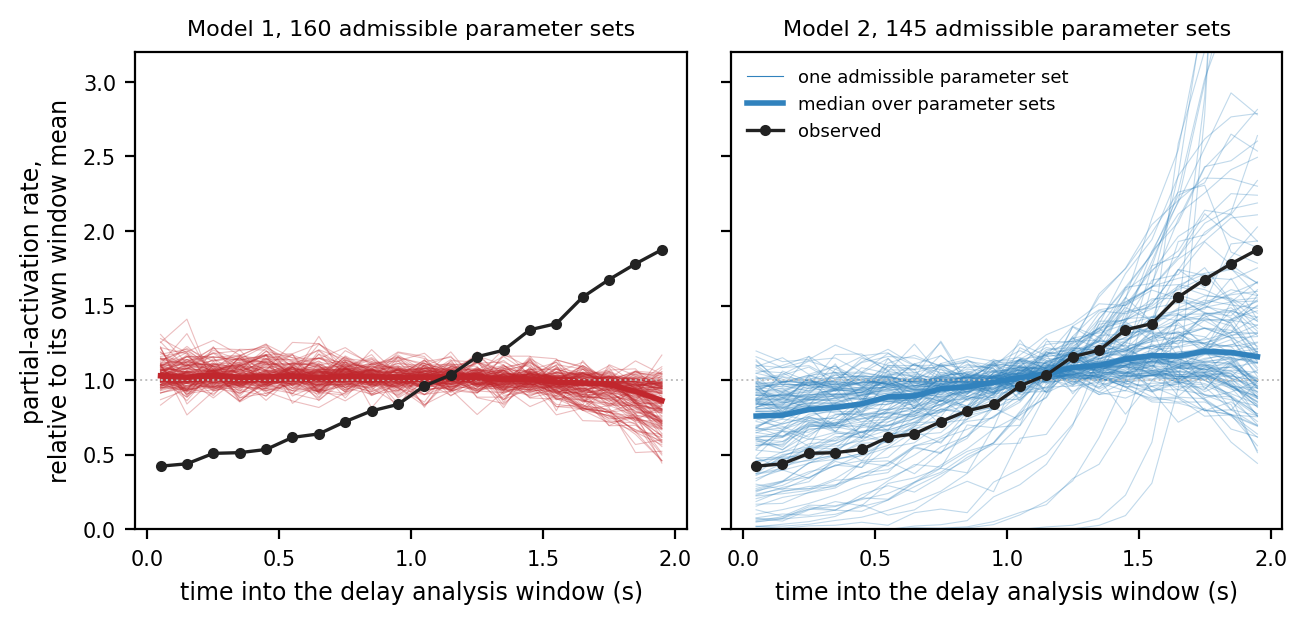
\includegraphics[width=\linewidth]{figures/fig10.png}\end{center}

\captionof{figure}{\textbf{P}\textbf{roportion of premature responses} \textbf{within a} \textbf{0.4 s window centered on response signal onset as a function of motion coherence and duration}\textbf{, averaged across subjects}\textbf{.}  Error bars represent $\pm$1 within-subjects standard error of the mean, computed using the method proposed by \textcite{moreyConfidenceIntervalsNormalized2008}.}\label{fig:premature}

\captionof{table}{\textbf{Full ANOVA results for response accuracy, mean response time (RT), mean pre-motor execution time (PMET), and mean motor execution time (MET). Two-way within-subject analyses of variance (duration $\times$ coherence, n = 22), Greenhouse--Geisser corrected wherever a factor has more than two levels, which is why those degrees of freedom are fractional; $\eta_{p}^{2}$ is the partial eta squared. Computed by run\_stats.R from the archive's own per-participant and per-condition exports.}}\label{tab:behav}

\begin{center}\small
\resizebox{\ifdim\width>\linewidth\linewidth\else\width\fi}{!}{%
\begin{tabular}{llllllll}
\toprule
Dependent variable & Effect tested &  & df1 & df2 & \emph{F} & \emph{p}-value & $\eta_{p}^{2}$ \\ \midrule
Accuracy & duration &  & 1 & 21 & 22.676 & \emph{p < .001} & 0.519 \\
 & coherence &  & 1.30 & 27.40 & 222.223 & \emph{p < .001} & 0.914 \\
 & duration $\times$ coherence &  & 1.96 & 41.24 & 12.171 & \emph{p < .001} & 0.367 \\
 &  &  &  &  &  &  &  \\
Mean RT & duration &  & 1 & 21 & 65.790 & \emph{p < .001} & 0.758 \\
 & coherence &  & 1.49 & 31.39 & 14.190 & \emph{p < .001} & 0.403 \\
 & duration $\times$ coherence &  & 1.68 & 35.25 & 4.607 & \emph{p = .022} & 0.180 \\
 &  &  &  &  &  &  &  \\
Mean PMET & duration &  & 1 & 21 & 69.600 & \emph{p < .001} & 0.768 \\
 & coherence &  & 1.60 & 33.50 & 14.000 & \emph{p < .001} & 0.400 \\
 & duration $\times$ coherence &  & 1.72 & 36.14 & 3.575 & \emph{p = .045} & 0.145 \\
 &  &  &  &  &  &  &  \\
Mean MET & duration &  & 1 & 21 & 1.095 & \emph{p = .307} & 0.050 \\
 & coherence &  & 1.51 & 31.73 & 0.624 & \emph{p = .499} & 0.029 \\
 & duration $\times$ coherence &  & 1.86 & 39.12 & 2.436 & \emph{p = .104} & 0.104 \\
\bottomrule
\end{tabular}
}
\end{center}
\emph{Note}.  A partial eta squared statistic  ($\eta_{p}^{2}$)  is reported as a measure of effect size. Degrees of freedom (df) with decimals indicate that a Greenhouse-Geisser correction was applied.

\captionof{table}{\textbf{Full ANOVA results for} \textbf{partial muscle activation rate in the electromyographic channel of the responding effector}  \textbf{across} \textbf{task periods}\textbf{.}}\label{tab:pma}

\begin{center}\small
\resizebox{\ifdim\width>\linewidth\linewidth\else\width\fi}{!}{%
\begin{tabular}{lllllll}
\toprule
Period & Effect tested & df1 & df2 & \emph{F} & \emph{p}-value & $\eta_{p}^{2}$ \\ \midrule
Stimulus & duration & 1 & 21 & 13.381 & \emph{p} =  .001 & 0.389 \\
 & coherence & 1.33 & 28.01 & 5.251 & \emph{p} =  .021 & 0.200 \\
 & time, linear & 1 & 21 & 30.869 & p < .001 & 0.595 \\
 & duration $\times$ coherence & 1.98 & 41.51 & 0.312 & \emph{p = .731} & -- \\
 & duration $\times$ time, linear & 1 & 21 & 9.532 & p = .006 & 0.312 \\
 & coherence $\times$ time, linear & 1.72 & 36.20 & 6.145 & p = .007 & 0.226 \\
 & duration $\times$ coherence $\times$ time, linear & 1.87 & 39.18 & 0.729 & p = .480 & 0.034 \\
 & time, quadratic & 1 & 21 & 2.621 & p = .120 & 0.111 \\
 & duration $\times$ time, quadratic & 1 & 21 & 3.555 & p = .073 & 0.145 \\
 & coherence $\times$ time, quadratic & 1.90 & 39.81 & 0.525 & p = .586 & 0.024 \\
 & duration $\times$ coherence $\times$ time, quadratic & 1.59 & 33.42 & 0.403 & p = .625 & 0.019 \\
 &  &  &  &  &  &  \\
Delay & duration & 1 & 21 & 33.186 & \emph{p}  < .001 & 0.612 \\
 & coherence & 1.96 & 41.15 & 3.361 & \emph{p = .045} & 0.138 \\
 & time, linear & 1 & 21 & 35.238 & p < .001 & 0.627 \\
 & duration $\times$ coherence & 1.92 & 40.42 & 3.474 & \emph{p = .042} & 0.142 \\
 & duration $\times$ time, linear & 1 & 21 & 11.898 & p = .002 & 0.362 \\
 & coherence $\times$ time, linear & 1.70 & 35.61 & 0.524 & p = .567 & 0.024 \\
 & duration $\times$ coherence $\times$ time, linear & 1.74 & 36.45 & 0.508 & p = .580 & 0.024 \\
 & time, quadratic & 1 & 21 & 18.891 & p < .001 & 0.474 \\
 & duration $\times$ time, quadratic & 1 & 21 & 0.751 & p = .396 & 0.035 \\
 & coherence $\times$ time, quadratic & 1.95 & 40.89 & 1.855 & p = .170 & 0.081 \\
 & duration $\times$ coherence $\times$ time, quadratic & 1.86 & 39.04 & 0.946 & p = .391 & 0.043 \\
 &  &  &  &  &  &  \\
Response signal & duration & 1 & 21 & 36.559 & \emph{p}  < .001 & 0.635 \\
 & coherence & 1.56 & 32.82 & 1.159 & \emph{p} =  .315 & -- \\
 & time & 1 & 21 & 21.964 & \emph{p}  < .001 & 0.511 \\
 & duration $\times$ coherence & 1.91 & 40.04 & 0.041 & \emph{p = .954} & -- \\
 & duration $\times$ time & 1 & 21 & 7.046 & \emph{p} =  .015 & 0.251 \\
 & coherence $\times$ time & 1.84 & 38.61 & 0.407 & \emph{p = .651} & -- \\
 & duration $\times$ coherence $\times$ time & 1.75 & 36.67 & 0.587 & \emph{p = .539} & -- \\
 &  &  &  &  &  &  \\
Response & duration & 1 & 21 & 7.613 & p = .012 & 0.266 \\
Response & coherence & 1.90 & 39.98 & 1.845 & p = .173 & 0.081 \\
Response & duration $\times$ coherence & 1.86 & 39.10 & 0.342 & p = .697 & 0.016 \\
\bottomrule
\end{tabular}
}
\end{center}
Note. Greenhouse--Geisser correction was applied to every effect with more than one numerator degree of freedom, that is to every effect involving the three-level coherence factor; degrees of freedom (df) with decimals indicate a corrected test. The partial eta squared statistic ($\eta_{p}^{2}$) is computed from the uncorrected degrees of freedom and is therefore unchanged by that correction. Time refers to the time bin factor. The time-bin main effect and its interactions are reported as one-degree-of-freedom linear-trend and quadratic contrasts computed on per-participant scores for the Stimulus and Delay periods (Methods): a contrast crossed only with duration therefore yields F(1,21), whereas a contrast crossed with coherence carries corrected degrees of freedom. The RS period is unaffected (only two time bins, so the omnibus and trend tests coincide exactly, and no quadratic contrast exists). The Response period is analyzed on its single informative bin, for which no time-bin factor, and therefore no trend or quadratic decomposition, applies (Methods).

\captionof{table}{\textbf{Full ANOVA results for} \textbf{the} \textbf{late}\textbf{ralized readiness potential} \textbf{amplitude}  \textbf{across} \textbf{task periods}\textbf{.}}\label{tab:lrp}

\begin{center}\small
\resizebox{\ifdim\width>\linewidth\linewidth\else\width\fi}{!}{%
\begin{tabular}{llllllll}
\toprule
Period & Effect tested &  & df1 & df2 & \emph{F} & \emph{p}-value & $\eta_{p}^{2}$ \\ \midrule
Stimulus & duration &  & 1 & 21 & 0.614 & \emph{p = .442} & -- \\
 & coherence &  & 1.75 & 36.66 & 1.498 & \emph{p = .237} & -- \\
 & time, linear &  & 1 & 21 & 0.497 & p = .489 & 0.023 \\
 & duration $\times$ coherence &  & 1.87 & 39.26 & 0.387 & \emph{p = .668} & -- \\
 & duration $\times$ time, linear &  & 1 & 21 & 2.222 & p = .151 & 0.096 \\
 & coherence $\times$ time, linear &  & 1.49 & 31.27 & 0.551 & p = .531 & 0.026 \\
 & duration $\times$ coherence $\times$ time, linear &  & 1.97 & 41.44 & 0.169 & p = .843 & 0.008 \\
 & time, quadratic &  & 1 & 21 & 0.487 & p = .493 & 0.023 \\
 & duration $\times$ time, quadratic &  & 1 & 21 & 7.201 & p = .014 & 0.255 \\
 & coherence $\times$ time, quadratic &  & 1.74 & 36.63 & 2.267 & p = .124 & 0.097 \\
 & duration $\times$ coherence $\times$ time, quadratic &  & 1.93 & 40.61 & 0.161 & p = .845 & 0.008 \\
 &  &  &  &  &  &  &  \\
Delay & duration &  & 1 & 21 & 0.019 & \emph{p} =  .892 & -- \\
 & coherence &  & 1.34 & 28.13 & 0.440 & \emph{p} =  .569 & -- \\
 & time, linear &  & 1 & 21 & 14.338 & p = .001 & 0.406 \\
 & duration $\times$ coherence &  & 1.96 & 41.16 & 0.378 & \emph{p = .683} & -- \\
 & duration $\times$ time, linear &  & 1 & 21 & 0.262 & p = .614 & 0.012 \\
 & coherence $\times$ time, linear &  & 1.56 & 32.72 & 0.283 & p = .701 & 0.013 \\
 & duration $\times$ coherence $\times$ time, linear &  & 1.90 & 39.84 & 0.031 & p = .964 & 0.001 \\
 & time, quadratic &  & 1 & 21 & 4.041 & p = .057 & 0.161 \\
 & duration $\times$ time, quadratic &  & 1 & 21 & 0.574 & p = .457 & 0.027 \\
 & coherence $\times$ time, quadratic &  & 1.93 & 40.62 & 0.682 & p = .506 & 0.031 \\
 & duration $\times$ coherence $\times$ time, quadratic &  & 1.98 & 41.67 & 0.330 & p = .719 & 0.015 \\
 &  &  &  &  &  &  &  \\
Response signal & duration &  & 1 & 21 & 0.185 & \emph{p} =  .671 & -- \\
 & coherence &  & 1.45 & 30.43 & 0.252 & \emph{p} =  .707 & -- \\
 & time &  & 1 & 21 & 14.076 & \emph{p} =  .001 & 0.401 \\
 & duration $\times$ coherence &  & 1.96 & 41.08 & 0.267 & \emph{p = .762} & -- \\
 & duration $\times$ time &  & 1 & 21 & 1.238 & \emph{p} =  .278 & -- \\
 & coherence $\times$ time &  & 1.59 & 33.39 & 1.058 & \emph{p = .344} & -- \\
 & duration $\times$ coherence $\times$ time &  & 1.94 & 40.83 & 0.108 & \emph{p = .893} & -- \\
 &  &  &  &  &  &  &  \\
Response & duration &  & 1 & 21 & 0.400 & \emph{p} =  .534 & -- \\
 & coherence &  & 1.55 & 32.45 & 0.309 & \emph{p} =  .680 & -- \\
 & time &  & 1 & 21 & 54.331 & \emph{p}  < .001 & 0.721 \\
 & duration $\times$ coherence &  & 1.97 & 41.30 & 0.666 & \emph{p = .517} & -- \\
 & duration $\times$ time &  & 1 & 21 & 4.129 & \emph{p} =  .055 & -- \\
 & coherence $\times$ time &  & 1.60 & 33.70 & 0.246 & \emph{p = .734} & -- \\
 & duration $\times$ coherence $\times$ time &  & 1.62 & 34.05 & 0.589 & \emph{p = .526} & -- \\
\bottomrule
\end{tabular}
}
\end{center}
Note. Conventions as in Table~\ref{tab:pma}.

\captionof{table}{\textbf{Full ANOVA results} \textbf{for} \textbf{mu--beta-band spectral amplitude lateralization} \textbf{across} \textbf{task periods}\textbf{.}}\label{tab:mbl}

\begin{center}\small
\resizebox{\ifdim\width>\linewidth\linewidth\else\width\fi}{!}{%
\begin{tabular}{llllllll}
\toprule
Period & Effect tested &  & df1 & df2 & \emph{F} & \emph{p}-value & $\eta_{p}^{2}$ \\ \midrule
Stimulus & duration &  & 1 & 21 & 2.146 & \emph{p} =  .158 & -- \\
 & coherence &  & 1.31 & 27.56 & 2.813 & \emph{p} =  .096 & -- \\
 & time, linear &  & 1 & 21 & 11.740 & p = .003 & 0.359 \\
 & duration $\times$ coherence &  & 1.62 & 34.00 & 0.755 & \emph{p = .452} & -- \\
 & duration $\times$ time, linear &  & 1 & 21 & 4.497 & p = .046 & 0.176 \\
 & coherence $\times$ time, linear &  & 1.95 & 40.99 & 0.517 & p = .596 & 0.024 \\
 & duration $\times$ coherence $\times$ time, linear &  & 1.85 & 38.90 & 0.021 & p = .974 & 0.001 \\
 & time, quadratic &  & 1 & 21 & 9.116 & p = .007 & 0.303 \\
 & duration $\times$ time, quadratic &  & 1 & 21 & 0.236 & p = .632 & 0.011 \\
 & coherence $\times$ time, quadratic &  & 1.66 & 34.89 & 1.936 & p = .165 & 0.084 \\
 & duration $\times$ coherence $\times$ time, quadratic &  & 1.99 & 41.79 & 1.302 & p = .283 & 0.058 \\
 &  &  &  &  &  &  &  \\
Delay & duration &  & 1 & 21 & 3.177 & \emph{p} =  .089 & -- \\
 & coherence &  & 1.29 & 27.12 & 1.257 & \emph{p} =  .285 & -- \\
 & time, linear &  & 1 & 21 & 7.107 & p = .014 & 0.253 \\
 & duration $\times$ coherence &  & 1.69 & 35.43 & 1.586 & \emph{p = .220} & -- \\
 & duration $\times$ time, linear &  & 1 & 21 & 0.019 & p = .893 & 0.001 \\
 & coherence $\times$ time, linear &  & 1.78 & 37.43 & 1.371 & p = .265 & 0.061 \\
 & duration $\times$ coherence $\times$ time, linear &  & 1.81 & 37.91 & 2.687 & p = .086 & 0.113 \\
 & time, quadratic &  & 1 & 21 & 3.290 & p = .084 & 0.135 \\
 & duration $\times$ time, quadratic &  & 1 & 21 & 3.741 & p = .067 & 0.151 \\
 & coherence $\times$ time, quadratic &  & 1.96 & 41.11 & 3.147 & p = .054 & 0.130 \\
 & duration $\times$ coherence $\times$ time, quadratic &  & 1.29 & 27.01 & 0.565 & p = .501 & 0.026 \\
 &  &  &  &  &  &  &  \\
Response signal & duration &  & 1 & 21 & 3.039 & \emph{p} =  .096 & -- \\
 & coherence &  & 1.90 & 39.94 & 0.160 & \emph{p = .843} & -- \\
 & time &  & 1 & 21 & 0.059 & \emph{p} =  .810 & -- \\
 & duration $\times$ coherence &  & 2.00 & 41.96 & 1.216 & \emph{p} =  .307 & -- \\
 & duration $\times$ time &  & 1 & 21 & 1.509 & \emph{p} =  .233 & -- \\
 & coherence $\times$ time &  & 1.99 & 41.73 & 0.024 & \emph{p = .976} & -- \\
 & duration $\times$ coherence $\times$ time &  & 1.66 & 34.93 & 1.458 & \emph{p = .246} & -- \\
 &  &  &  &  &  &  &  \\
Response & duration &  & 1 & 21 & 0.006 & \emph{p} =  .937 & -- \\
 & coherence &  & 1.95 & 40.91 & 0.364 & \emph{p = .692} & -- \\
 & time &  & 1 & 21 & 11.658 & \emph{p}  = .003 & 0.357 \\
 & duration $\times$ coherence &  & 1.65 & 34.56 & 0.161 & \emph{p = .811} & -- \\
 & duration $\times$ time &  & 1 & 21 & 2.129 & \emph{p} =  .159 & -- \\
 & coherence $\times$ time &  & 1.98 & 41.51 & 0.252 & \emph{p = .776} & -- \\
 & duration $\times$ coherence $\times$ time &  & 1.72 & 36.21 & 0.719 & \emph{p = .475} & -- \\
\bottomrule
\end{tabular}
}
\end{center}
Note. Conventions as in Table~\ref{tab:pma}. One stimulus-period effect (coherence $\times$ time, linear) is significant on the omnibus test (p < .001) but not as a full-window linear trend (p = .596), because the effect is confined to the first half of the stimulus period (Results; Table~\ref{tab:split}). One other (duration $\times$ time, linear) is significant as a linear trend (p = .046) but was not on the omnibus test (p = .136).

\captionof{table}{\textbf{Mu--beta lateralization, stimulus period: split-half trend analysis.}}\label{tab:split}

A non-monotone profile for this measure was anticipated in Methods (rising over approximately the first second of the stimulus period and flattening thereafter), which is why a quadratic contrast was prespecified alongside the linear one. To characterize this directly, the stimulus period was split a priori at its temporal midpoint into two 1-s halves (bins 1--10 and 11--20) and the same TREND analysis was repeated within each half:

\begin{center}\small
\resizebox{\ifdim\width>\linewidth\linewidth\else\width\fi}{!}{%
\begin{tabular}{lllllll}
\toprule
Window & trend F & trend p & trend $\times$ coherence F & trend $\times$ coherence p & trend $\times$ duration F & trend $\times$ duration p \\ \midrule
first half (0--1 s) & 11.19 & .003 & 5.76 & .018 & 5.67 & .027 \\
second half (1--2 s) & 2.22 & .151 & 0.37 & .658 & 5.34 & .031 \\
\bottomrule
\end{tabular}
}
\end{center}
The coherence-dependent trend is present in the first half (linear trend $\times$ coherence significant) and extinguished in the second half (same contrast null), while the duration-dependent trend holds in both halves. This is the pattern expected if coherence-dependent trajectories are converging on a common sustained level rather than ramping at a constant, coherence-dependent rate throughout the period: the full-window test in Table~\ref{tab:mbl} above, which averages across both halves, accordingly shows neither a significant linear nor quadratic coherence $\times$ time trend.

\end{document}
